\documentclass[fontsize=12pt,abstract=on,titlepage,bibliography=totoc,ngerman,listof=totoc]{scrreprt}

%\usepackage[utf8]{inputenc}
\usepackage[onehalfspacing]{setspace}
\usepackage[ngerman]{babel}
\usepackage{fontspec}
\usepackage[a4paper, left=3cm, right=3cm, top=3cm]{geometry}
\usepackage{amsmath}
%\usepackage{qtree}
\usepackage{listings}
\usepackage{floatrow}
%\usepackage{capt-of}
\usepackage{fancyvrb}
\usepackage{graphicx}
\usepackage[section]{placeins}
\usepackage{url}
\usepackage{multirow}
\usepackage{arydshln}
\usepackage[style=alphabetic-verb,backend=biber]{biblatex}
\usepackage{rotating}
\usepackage{tocloft}
\usepackage{tocbasic}

\setlength{\parindent}{10pt} 
\floatstyle{plain}

\newfloat{program}{thp}{lop}
\floatname{program}{Beispiel}

\interfootnotelinepenalty=10000

\setlength{\cftbeforetoctitleskip}{50pt} 

\renewcommand{\abstractname}{Zusammenfassung}

\urldef\persalatin\url{http://www.perseus.tufts.edu/hopper/text?doc=Perseus%3atext%3a1999.04.0059}
\urldef\perselemlat\url{http://www.perseus.tufts.edu/hopper/text?doc=Perseus%3atext%3a1999.04.0060}
\urldef\vatlatinitas\url{http://www.vatican.va/roman_curia/institutions_connected/latinitas/documents/rc_latinitas_20040601_lexicon_it.html}
\lstdefinelanguage{gf}
{
  morekeywords={abstract, flags, cat, fun, incomplete, concrete, of, open, in, lincat, lin, resource, param, oper, variants, table, interface, instance, def, data, lindef, printname,},
  sensitive=false,
  morecomment=[l]{--},
  morestring=[b]",
  stringstyle={\textit}
}
\lstset{language=gf,captionpos=b,numbers=left, numberstyle=\tiny, numbersep=5pt, basicstyle=\ttfamily}

\bibliography{MA.ebib}
\begin{document}
\setcounter{tocdepth}{2}
\date{31.10.2013}
\makeatletter
\begin{titlepage}
{\sffamily
  \begin{center}
    \vspace{4cm}
    \begin{huge}
      Hausarbeit \\
      zur Erlangung des Magistergrades \\
      an der Ludwig-Maximilians-Universität München \\[3cm]
    \end{huge}
    {\Huge Erstellen einer Lateingrammatik im Grammatical Framework \\[4cm] }
    {\LARGE vorgelegt von Herbert Lange \\ Matrikelnummer 8063320 \\[3.5cm] }
  \end{center}
  \parindent0mm
  \begin{huge} 
    Fach: Computerlinguistik  \\[0.5cm]
    Referent: Prof. Dr. Klaus U. Schulz \\[0.5cm]
    München, den \@date 
  \end{huge}
}
\end{titlepage}
\begin{abstract}
In dieser Arbeit sollen an einem konkreten Beispiel die nötigen Schritte gezeigt werden, um eine computergestützte Grammatik für eine natürliche Sprache zu entwerfen. Am Beispiel der lateinischen Sprache wird gezeigt, wie eine Grammatik, bestehend aus einem Lexikon, einem Morphologiesystem und einer Syntax, implementiert werden kann, die sich in ein größeres, multilinguales Grammatiksystem einpassen lässt. Dadurch können zum einen in der implementierten Sprache Sätze verarbeitet werden, aber auch in jede andere im System vorhandene Sprache übersetzt werden. Gezeigt wird ein rein regelbasierter Ansatz der sich von den statistischen Methoden durch seine Striktheit und Beschränktheit, aber auch durch seine Zuverlässigkeit abhebt.
\end{abstract}
\makeatother
\tableofcontents
%\pagebreak
\clearpage
\setcounter{page}{1}
\chapter{Einleitung}
\label{chap:einleitung}
\section{Motivation}
\label{sec:motivation}
Im Bereich der Computerlinguistik haben sich im Laufe der Zeit zwei Lager gebildet, die jeweils ihren Ansatz zur Sprachverarbeitung vertreten. Der heute häufiger anzutreffende Ansatz ist der statistische Ansatz, denn nach aktuellem Stand kann man durch statistische Methoden in der Sprachverarbeitung mit relativ geringem Aufwand brauchbare bis gute Ergebnisse erzielen. Allerdings bedarf der statistische Ansatz möglichst gute Trainingsdaten, die nicht immer leicht zu beschaffen und zu bewerten sind. \par
Der zweite, ältere Ansatz, ist die regelbasierte Sprachverarbeitung. Er prägte die Anfänge der Computerlinguistik stark, wurde jedoch im Laufe der Zeit vom statistischen Ansatz verdrängt. Dies ist unter anderem auf die steigende Leistung heutiger Rechner zur Verarbeitung großer Datenmengen und vor allem die Fülle an Daten, die über das Internet verfügbar sind. Die Grundlagen regelbasierter Grammatiken sind in etwa so alt wie die Wissenschaft der Linguistik selbst und sollte auch weiterhin zum Wissen eines jeden Computerlinguisten gehören. \par
In dieser Arbeit sollen an einem konkreten Beispiel die nötigen Schritte gezeigt werden, um eine computergestützte Grammatik für eine natürliche Sprache zu entwerfen. Am Beispiel der lateinischen Sprache wird gezeigt, wie ein Lexikon, ein Morphologiesystem und eine Syntax implementiert werden kann, die sich in ein größeres, multilinguales Grammatiksystem einfügen lässt. Vor allem eine Sprache wie Latein, die zum einen für ihre Regelmäßigkeit aber auch für ihre linguistischen Besonderheiten bekannt ist, kann zu interessanten Erkenntnissen im Bereich der Grammatikentwicklung führen. \par
Ein weiterer Aspekt war es, einen kleinen Beitrag zu einem größeren Projekt zu leisten. Denn die lateinische Sprache war im Grammatical Framework\footnote{\url{http://www.grammaticalframework.org/}}, dem für diese Arbeit gewählten multilingualem Grammatik-, Parsing- und Übersetzungssystem, noch nicht in einem funktionsfähigen Umfang vorhanden.
\pagebreak
\section{Ziel der Arbeit}
\label{sec:ziel}
Ziel dieser Arbeit ist es, zum einen eine soweit funktionstüchtiges Grammatiksystem zu entwickeln, dass es in der Lage ist grundlegende Sätze zu verarbeiten und durch die Integration in ein multilinguales Grammatiksystem in andere, moderne, Sprachen zu übersetzen. Zum anderen sollen aber auch die allgemeinen Schritte einer Grammatikentwicklung exemplarisch an der lateinischen Sprache dargelegt werden. \par
Der Schwerpunkt soll dabei zum einen auf der Nähe zu einer gewöhnlichen, im bayerischen Schulunterricht verwendeten, lateinischen Schulgrammatik liegen. Dies spiegelt sich, zum einen teilweise in der Abfolge der Schritte, zum anderen in einigen Entscheidungen beim Entwurf der Grammatik, wieder. So ist eine lateinische Grammatik grob in folgende Abschnitte unterteilt: Phonologie, Wortarten und Wortbildung, Morphologie uns Syntax. Zwar werden die ersten drei Teile in dieser Arbeit größtenteils vernachlässigt, die logische Folge der zwei verbleibenden Teile wird aber auch hier beibehalten. Allerdings wird der in Grammatiken nicht in dieser Form auffindbare Teil über die Lexikonentwicklung ihnen vorangestellt. \par
Zum anderen sollen, um die Verwendung im multilingualen Grammatiksystem des Grammatical Framework ermöglichen zu können, möglichst große Teile der für eine Sprache geforderten Schnittstellen zur Verfügung gestellt werden. Dies beeinflusst ebenfalls die Struktur der Arbeit, durch die Gliederung einer Grammatik in gewisse Module. 
\pagebreak
\section{Aufbau der Arbeit}
\label{sec:aufbau}
Zu Beginn der Arbeit werden in Kapitel \ref{chap:grundlagen} die nötigen Grundlagen für die weiteren Teile der Arbeit erörtert. Zunächst einmal werden die Grundlagen des Grammatical Framework in Abschnitt \ref{sec:gf} erklärt. Zuerst eine grundlegende Beschreibung des Umfangs und der Funktionen dieses Programmpakets. Anschließend folgt eine Einführung in den Formalismus der bei der Entwicklung der Grammatiken für das Grammatical Framework verwendet wird. Und dieser Abschnitt wird mit einigen Informationen zur Ressource Grammar Library, der multilingualen Grammatikbibliothek des Grammatical Frameworks abgeschlossen. Nach den technischeren Grundlagen folgen einige Informationen zur lateinischen Sprache in Abschnitt \ref{sec:latein}. Zunächst erfolgt eine sprachwissenschaftliche Einordnung dieser Sprache unter besonderer Hervorhebung einiger interessanter Merkmale. Darauf folgt ein kurzer Abschnitt, der die Relevanz dieser als tot geltenden Sprache in der heutigen Zeit beleuchtet. \par
Nach dieser allgemeinen Einführung erfolgt im nächsten großen Teil, dem Kapitel \ref{chap:grammatik}, die Beschreibung der nötigen Schritte, die umgesetzt wurden um eine Lateingrammatik im Grammatical Framework zu entwickelt. Es ist in die drei Abschnitte Lexikon, Morphologie und Syntax unterteilt, da dies drei getrennte Module in der Ressource Grammar Library bilden. Bei der Entwicklung er Grammatik zeigten sich allerdings oft Abhängigkeiten zwischen den drei Bestandteilen, so dass im laufe der Zeit auch Änderungen in anderen Komponenten nötig waren. Im Abschnitt \ref{sec:lexikon} wird dargestellt, wie das Lexikon, das für eine Grammatik im Grammatical Framework nötig ist, erstellt wird. Darauf folgt in Abschnitt \ref{sec:morpho} die Beschreibung der lateinischen Wortflexion, wie sie im Grammatical Framework umgesetzt werden kann. Als letzter Teil dieses Kapitels wird in Abschnitt \ref{sec:syntax} erläutert, welche syntaktischen Regeln in der Grammatik nötig waren um eine funktionierende Grammatik zu erhalten, was ja zu den Hauptzielen dieser Arbeit gehörte. \par
Abgerundet wird die Arbeit in Kapitel \ref{chap:ausblick}, in dem ein Fazit der Arbeit gezogen und ein Ausblick auf Erweiterung und Verwendung gegeben wird. So wird gezeigt, welchen Sprachumfang die Grammatik bisher umfasst, welche Erweiterungen möglichst gewinnbringend sein können und auch in welchen Bereichen das Ergebnis dieser Arbeit Anwendung finden kann.
% \pagebreak
\chapter{Grundlagen}
\label{chap:grundlagen}
\section{Das Grammatical Framework}
\label{sec:gf}
Das Grammatical Framework ist ein Softwaresystem mit einer spezialisierten Programmiersprache zur Entwicklung von Grammatiken. Es benutzt Formalismen, wie sie auch in modernen funktionalen Programmiersprachen wie Haskell zu finden sind, unterstützt aber vor allem die Entwicklung von Anwendungen zur Verarbeitung natürlicher Sprachen.\footnote{vgl. \cite{RANTA2011} S. vii} Somit können einem manche Konzepte bereits vertraut sein, wenn man sich schon mit den Möglichkeiten der funktionalen Programmierung\footnote{Beispiele für funktionale Programmiersprachen sind Lisp, SML und Haskell} auseinander gesetzt hat. Ein großer Vorteil des Grammatical Frameworks im Vergleich zu anderen Parsingsystemen ist, dass durch das Typsystem, das unter anderem auf der Typtheorie von Martin-Löf basiert, Grammatikfehler schon durch den Compiler erkannt werden können.\footnote{vgl. \cite{RANTA2011} S. 127ff.} \par
Die große Stärke des Grammatical Frameworks ist die Multilingualität. Das Grundkonzept für die Unterstützung verschiedener Sprachen ist die Trennung in eine konkrete und eine abstrakte Repräsentation der Grammatik. Dabei haben die unterschiedlichen Sprachen eine gemeinsame abstrakte Struktur. Die konkrete Syntax dagegen beschreibt, wie aus einer sprachunabhängigen Repräsentation eines "`Satzes"' eine für die jeweilige Sprache spezifische Zeichenkette erzeugt werden kann. Über diesen Schritt der abstrakten Repräsentation kann man eine Übersetzung zwischen verschiedensten Sprachen umsetzen, die eine gemeinsame abstrakte Syntax teilen.\footnote{vgl. \cite{RANTA2011} S. 10ff.} Die Details dieses Formalismus sollen nun an einigen kleinen deutsch-englischen Beispielen genauer betrachtet werden.
\pagebreak
\subsection{Der Grammatikformalismus}
\label{subsec:grammatik}
Im Bereich der Computerlinguistik und Informatik werden hauptsächlich kontextfreie Grammatiken, also Grammatiken von Typ 2 der Chomsky-Hierarchie, verwendet.\footnote{vgl. \cite{SCHOENING2008} S. 9f} Die zwei Hauptgründe dafür sind, dass die Mächtigkeit dieses Formalismuses meist ausreicht, die gewünschten Sprachen zu beschreiben. So sind in kontextfreien Sprachen geklammerte Ausdrücke möglich, die bei Programmiersprachen recht häufig sind.\footnote{vgl. \cite{SCHOENING2008} S. 43} Zudem ist der Verarbeitungsaufwand gering im Vergleich zu Grammatiken einer der höheren Stufen, und es existieren effiziente Algorithmen zum Parsen mit kontextfreien Grammatiken, so z.B. der Cocke-Younger-Kasami-Algorithmus, auch bekannt als CYK-Algorithmus.\footnote{vgl. \cite{SCHOENING2008} S. 56f.}
\begin{program}[h!tp]
\begin{tabular}{llll}
1 & S & $\longrightarrow$ & NP, VP \\
2 & NP & $\longrightarrow$ & Det, N \\
3 & N & $\longrightarrow$ & \textit{Mann} \\
4 & Det & $\longrightarrow$ & \textit{der} \\
5 & VP & $\longrightarrow$ & V \\
6 & V  & $\longrightarrow$ & \textit{schläft} \\
\end{tabular}
\caption{Kurzes Beispiel einer kontextfreien Grammatik}
\label{CFG-Beispiel}
\end{program}
Die in Beispiel \ref{CFG-Beispiel} gegebene Grammatik ist ein sehr minimalistisches Beispiel für eine kontextfreie Grammatik. Mit ihrer Hilfe kann nur der eine deutsche Satz "`Der Mann schläft"' hergeleitet werden. Eine mögliche Ableitung hat die in Beispiel \ref{CFG-Ableitung} gezeigte Form. Bei dieser Ableitung wurde top-down vorgegangen, also von der allgemeinsten Kategorie hinab bis zur spezifischen Zeichenkette. Alternativ wäre es auch möglich gewesen, eine bottom-up-Ableitung anzugeben, die lediglich dem Ablesen der gegebenen Ableitung von unten nach oben entspricht. In der Grammatik sind die Regeln zum einfacheren Bezug auf die Grammatik mit Regelnummern versehen. Diese Regelnummern sind deshalb auch in der Ableitung und dem entsprechenden Syntaxbaum zu sehen. \par
\begin{program}[h!tp]
\begin{Verbatim}[commandchars=\\\{\},codes={\catcode`$=3\catcode`^=7}] 
                    S
                    $\overset{1}{\Rightarrow}$ NP VP
                    $\overset{2}{\Rightarrow}$ Det N VP
                    $\overset{4}{\Rightarrow}$ \textit{der} N VP
                    $\overset{3}{\Rightarrow}$ \textit{der Mann} VP
                    $\overset{5}{\Rightarrow}$ \textit{der Mann} V
                    $\overset{6}{\Rightarrow}$ \textit{der Mann schläft}
\end{Verbatim}
\caption{Ableitung des Satzes mit Hilfe der Grammatik aus Beispiel \ref{CFG-Beispiel}}
\label{CFG-Ableitung}
\end{program}
% $ Just to fix errors in syntax highlighting
\begin{figure}[h!tp]
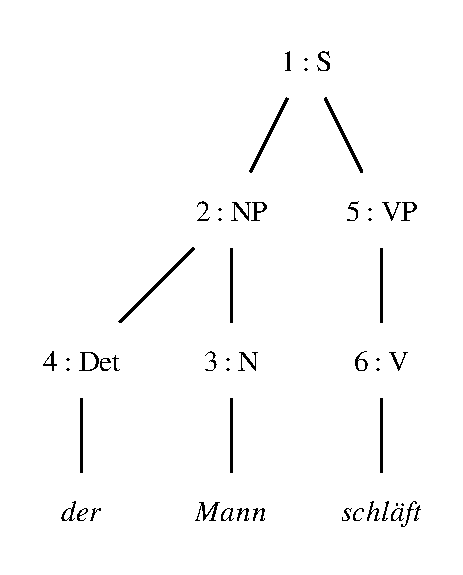
\includegraphics{graphics/MiniSatzSyntax.eps}
\caption{Syntaxbaum für die Ableitung in Beispiel \ref{CFG-Ableitung}}
\label{CFG-Syntaxbaum}
\end{figure}
Im Formalismus des Grammatical Framework wird die oben gegebene Grammatik in eine abstrakte und eine konkrete Syntax zerlegt. So entspricht diese abstrakte Syntax in etwa dem Syntaxbaum in Abbildung \ref{CFG-Syntaxbaum} ohne die terminalen Blätter. \par
% Listing MiniSatzAbs
\lstinputlisting[float=h!tp,caption={Abstrakte Syntax der Grammatik aus Beispiel \ref{CFG-Beispiel}},label={GF-MiniSatzAbs}]{minisatz/MiniSatzAbs.gf}
Die abstrakte Syntax der kontextfreien Grammatik aus Beispiel \ref{CFG-Beispiel} ist in Listing \ref{GF-MiniSatzAbs} zu sehen. Zunächst gibt das Schlüsselwort \texttt{abstract} an, dass es sich um eine Datei mit einer abstrakten Syntaxbeschreibung handelt. Diesem Schlüsselwort folgt der Name und nach dem \texttt{=} der Inhalt der Grammatik. \par
Zuerst werden mit Hilfe der \texttt{flags}-Direktive einige mögliche Einstellungen vorgenommen. In diesem sehr kurzen Beispiel wird nur die Startkategorie für das Parsing gesetzt, also die Wurzel aller Parsebäume. Andere mögliche Optionen sind z.B. die Einstellungen des Encodings und der Lexer, also das Programm, das die Eingabe in lexikalische Tokens zerlegt.\footnote{vgl. \cite{RANTA2011} S. 54f.} \par
Nach dem Schlüsselwort \texttt{cat} folgt eine Liste der Kategorien oder auch Non-Terminal-Symbole. Sie entsprechen Datentypdefinition in (funktionalen) Programmiersprachen. \par
Hauptbestandteil der Grammatik sind die Syntaxregeln. Sie werden nach dem Schlüsselwort \texttt{fun} aufgelistet. Die Regeln ähneln der Form von Funktionssignaturen in Sprachen wie Standard ML oder Haskell, denn sie beschreiben lediglich die Bestandteile, aus denen ein Ausdruck einer neuen Kategorie zusammengesetzt werden soll. Das genaue Vorgehen für die Kombination dieser Bestandteile wird dann sprachspezifisch in jeder konkreten Grammatik, die diese abstrakte Grammatik implementiert, beschrieben. So sagt die erste Regel mit dem Namen \texttt{mkNP} aus, dass ein Ausdruck der Kategorie \texttt{NP} aus einem Ausdruck der Kategorie \texttt{Det} und aus einem Ausdruck der Kategorie \texttt{N} zusammengesetzt werden kann. Dabei ist aber noch keine Aussage über die endgültige Reihenfolge der Bestandteile in konkreten Zeichenketten getroffen. Die letzten drei Regeln führen lediglich die lexikalische Einheiten mit einer entsprechenden Kategorie ein. \par
Diese abstrakte Grammatik kann nun konkret umgesetzt werden. Zwei konkrete Implementierungen, für Deutsch und Englisch, sind in Listing \ref{GF-MiniSatzGer} und \ref{GF-MiniSatzEng} zu finden. \par
% Listing MiniSatzGer
\lstinputlisting[float=h!tp,caption={Konkrete deutsche Syntax für die abstrakte Syntax in Listing \ref{GF-MiniSatzAbs}},label={GF-MiniSatzGer}]{minisatz/MiniSatzGer.gf}
% Listing MiniSatzEng
\lstinputlisting[float=h!tp,caption={Konkrete englische Syntax für die abstrakte Syntax in Listing \ref{GF-MiniSatzAbs}},label={GF-MiniSatzEng}]{minisatz/MiniSatzEng.gf}
Zunächst weist das Schlüsselwort \texttt{concrete} die Grammatik als eine konkrete Grammatik aus. Es folgt wie bei einer abstrakten Syntax der Name der Grammatik, diesmal wird jedoch darauf folgend angegeben, welche abstrakte Grammatik die Grundlage bietet, hier unsere \texttt{MiniSatzAbs}-Grammatik. \par
Das in der deutschen, konkreten Grammatik verwendete Flag \texttt{coding} ermöglicht es, die Zeichenkodierung in den Zeichenketten festzulegen. In diesem Falle ist es für die deutschen Umlaute nötig, die Zeichenkodierung anzugeben. Für andere Sprachen mit komplett vom lateinischen unterschiedlichen Schriftsystemen gibt es auch die Möglichkeit, statt der direkten Zeichenkodierung eine Transliteration zu verwenden. Dafür wird eine bijektive Abbildung zwischen Unicode-Zeichen und Zeichenketten der Länge eins oder größer, die nur aus ASCII-Zeichen bestehen, verwendet.\footnote{vgl. \cite{RANTA2011} S. 55 und S. 227f.} \par
Das Schlüsselwort \texttt{lincat} ist die konkrete Entsprechung zum Schlüsselwort \texttt{cat} in der abstrakten Syntax. Hier muss für jede in der abstrakten Syntax angegebene Kategorie ein konkreter Datentyp angegeben werden. In diesem Falle wurde für alle Kategorien der einfache Datentyp \texttt{Str}, also eine einfache Zeichenkette\footnote{Um genau zu sein, eine Liste von Token, die bei der Linearisierung mit Leerzeichen konkateniert werden}, gewählt. Das Grammatical Framework unterstützt auch verschiedene Arten komplexer Datentypen, die später näher erläutert werden. \par
Auf den \texttt{lincat}-Block folgt, mit dem Schlüsselwort \texttt{lin} markiert, der Abschnitt, in dem die für jede abstrakte Syntaxregel beschrieben wird, wie diese in eine konkrete Zeichenkette zu übersetzen ist. Für die drei lexikalischen Regeln \texttt{Mann\_N}, \texttt{der\_Det} und \texttt{schlafen\_N} ist dies lediglich die entsprechende Zeichenkette z.B. für \texttt{Mann\_N} "`Mann"' im Deutschen bzw. "`man"' im Englischen. Die restlichen Syntaxregeln sind in diesem Beispiel nur geringfügig komplexer. Die Regel \texttt{mkVP} gibt lediglich den Parameter als Rückgabewert zurück, bildet also die gleiche Zeichenkette, der bereits als Parameter übergeben wurde. Und die beiden verbleibenden Regeln \texttt{mkNP} und \texttt{mkS} konkatenieren einfach mit Hilfe des Operators \texttt{++} die beiden als Parameter übergebenen Zeichenketten. \par
Man kann diese sehr kurzen konkreten Grammatiken zusammen mit der gemeinsamen Grammatik in das Grammatical Framework laden und in einer der beiden Sprachen den Satz "`der Mann schläft"' bzw. "`the man sleeps"' parsen und die so erhaltene abstrakte Repräsentation \texttt{(mkS (mkNP der\_Det Mann\_N) (mkVP schlafen\_V))} in die andere Sprache linearisieren, also mit Hilfe der konkreten Syntaxregeln die entsprechende Zeichenkette in der Sprache generieren. \par
\begin{figure}
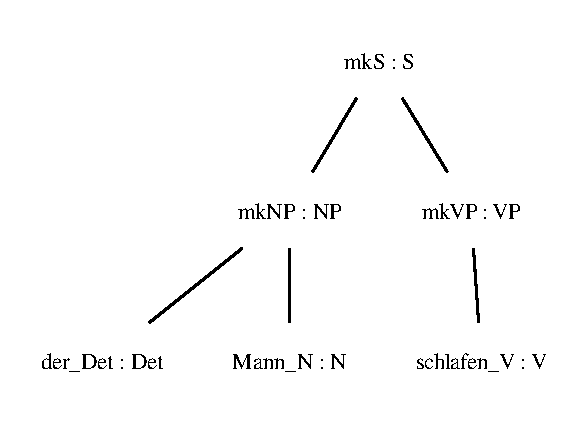
\includegraphics{graphics/MiniSatzTree.eps}
\caption{Baum der abstrakten Syntax für den Satz "`der Mann schläft"'}\label{MiniSatz-AbsTree}
\end{figure}
\begin{figure}
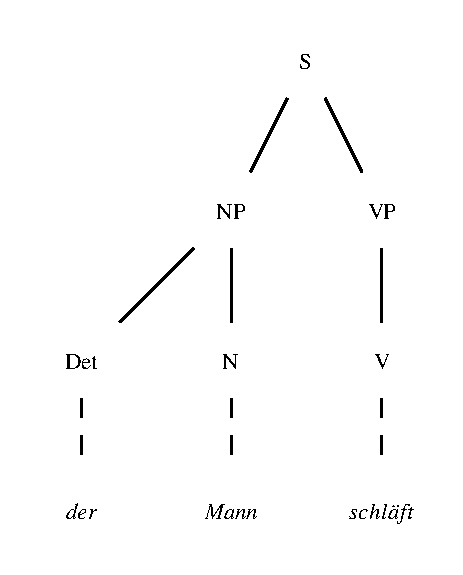
\includegraphics{graphics/MiniSatzParseGer.eps}
\caption{Parsebaum der konkreten deutschen Syntax}\label{MiniSatz-ParseGer}
\end{figure}
Mit Hilfe des Grammatical Frameworks kann man sich sowohl den abstrakten Syntaxbaum und als auch den konkreten Parsebaum für eine der implementierten Sprachen grafisch darstellen lassen. Diese Bäume für die MiniSatz-Grammatik sind in Abb. \ref{MiniSatz-AbsTree} und \ref{MiniSatz-ParseGer} zu sehen. \par
% Listing SatzAbs
\lstinputlisting[float=h!tp,caption={Aus Listing \ref{GF-MiniSatzAbs} erweiterte abstrakte Syntax \texttt{SatzAbs}},label={GF-SatzAbs}]{satz/SatzAbs.gf}
Nun kann man diese doch sehr minimalistische Grammatik etwas erweitern, so dass man auch die Sätze "`die Frauen schlafen"', "`der Mann sieht die Frau"' und "`der Mann liest das Buch"' erkennen kann. Die fertigen Quelltextdateien sind in Listing \ref{GF-SatzAbs}, \ref{GF-SatzGer} und \ref{GF-SatzEng} zu finden. Die Veränderungen in der abstrakten Syntax (Listing \ref{GF-SatzAbs}) betreffen hauptsächlich die Einführung von transitiven Verben mit der Kategorie \texttt{V2}. Mit der Funktion \texttt{mkVP2} wird aus einem transitiven Verb und einer Nominalphrase eine Verbalphrase mit Akkusativobjekt aufgebaut. Um auch Nominalphrasen im Plural zu ermöglichen, wird für den bestimmten Artikel eine Singular- und eine Pluralform benötigt. Auch das "`Lexikon"', also die Liste der lexikalischen Einheiten, wird um die Wörter für "`Frau"', "`Buch"', "`sehen"' und "`lesen"' erweitert. \par
% Listing SatzGer
\lstinputlisting[float=h!tp,caption={Erweiterte konkrete deutsche Syntax  \texttt{SatzGer}},label={GF-SatzGer},basicstyle=\footnotesize]{satz/SatzGer.gf}
In der konkreten Umsetzung sind nun aber größere Unterschiede, sowohl zur ursprünglichen Grammatik, als auch zwischen den unterschiedlichen Sprachen zu finden. Bei der konkreten deutschen Grammatik werden zuerst nach dem Schlüsselwort \texttt{param} drei neue Datentypen dadurch definiert, dass ihr Wertebereich aufgezählt wird. So wird definiert, dass im Deutschen der Genus die drei Werte Maskulin, Feminin, und Neutrum annehmen kann, der Numerus die Werte Singular und Plural und in diesem Beispiel Kasus die zwei Werte Nominativ und Akkusativ. Alle weiteren Fälle werden in diesem kleinen Beispiel nicht benötigt. Die nächste größere Änderung ist im \texttt{lincat}-Block zu finden. Denn statt allen Kategorien den selben einfachen Datentyp zu geben, haben nun alle Kategorien einen komplexen Typ. Zunächst sind all diese Typen Verbundtypen, in Englisch Records, zu erkennen an den geschweiften Klammern. Sie sammeln Objekte\footnote{Der Begriff Objekt wird, obwohl es sich bei dem Grammatical Framework nicht um eine objekt-orientierte Programmiersprache handelt, für Konstrukte eines bestimmten Typs verwendet} möglicherweise verschiedenen Typs in einem einzigen Objekt zusammen. Jedes dieser inneren Objekte hat einen Typ und einen Bezeichner, über den darauf zugegriffen werden kann.\footnote{Verbundtypen haben die Form \texttt{\{$l_1 : T_1 ; \dots ; l_n : T_n$\}} mit $l_1, \dots, l_n$ endlich viele verschiedenen Bezeichnern und $T_1, \dots, T_n$ beliebige Typen. Objekte dieser Typen haben die Form \texttt{\{$l_1 = v_1 ; \dots ; l_n = v_n$\}} mit $v_i$ Werte vom Typ $T_i$ für jedes $i$ mit $1\leq i\leq n$ (vgl. \cite{RANTA2011} S. 279)} Auf diese Weise haben z.B. Nomen ein inhärentes Genus, gespeichert im Bezeichner \texttt{g}, und eine Form, die hier nur vom Numerus abhängig ist, gespeichert im Bezeichner \texttt{s}. Üblicherweise ist die Nomenform auch vom Kasus abhängig, allerdings betrachten wir nur die beiden Kasus Nominativ und Akkusativ, bei denen hier die Nomen immer die selbe Form bilden. Nach diesem Schema sind die Typen für alle Kategorien aufgebaut. Um die Abhängigkeit eines Wertes von gewissen anderen Werten auszudrücken, gibt es im Grammatical Framework die so genannten Tabellentypen\footnote{Tabellentypen haben die Form \texttt{\{$Typ_1$ => $Typ_2$\}} mit $Typ_1,Typ,2$ beliebige Typen und Tabellenobjekte die Form \texttt{table \{ $k_1 => V_1 ; \dots ; k_n => V_n$ \}} mit $k_i$ von $Typ_1$ und $V_i$ vom $Typ_2$ (Tabellentypen sind im Grammatical Framework Sonderfälle von Funktionen, weswegen in dieser Arbeit nicht genauer auf die Funktionsweise eingegangen werden soll. Details sind bei \cite{RANTA2011} S. 281f. zu finden)}, wie sie auch bei den \texttt{s}-Feldern von \textit{Det}, \textit{N}, \textit{NP}, etc. zu sehen ist. Dies bedeutet, dass der Wert aus dem Bereich von $Typ_2$ vom Wert aus dem Bereich $Typ_1$ abhängt.\footnote{vgl. \cite{RANTA2011} S. 59} \par
Um es noch einmal zusammenzufassen, die Typen für die Kategorien im \texttt{licat}-""Bereich sind nun statt des einfachen Typs \texttt{Str} Verbundtypen, bestehend aus mehreren Objekten, deren Werte wiederum von anderen Werten abhängig sein können. Wie das konkret funktioniert, wird im nächsten Abschnitt sichtbar. Denn es müssen sowohl für die Verbundtypen als auch für die Tabellentypen konkrete Objekte erzeugt werden. Dies geschieht im \texttt{lin}-Block, in dem nun die konkreten Grammatikregeln "`konstruiert"' werden. Fangen wir am besten von hinten, also von den lexikalischen Regeln her, an. Der Typ für Verben, ungeachtet ob es transitive, also \texttt{V2}-Verben, oder intransitive \texttt{V}-Verben sind, gibt an, dass sie aus einem einzigen Tabellenobjekt mit dem Bezeichner \texttt{s} bestehen. Diese Tabelle hat den Typ \texttt{Numerus => Str}, also eine \texttt{Str}-Zeichenkette, deren Wert von einem Numerus abhängt. Üblicherweise enthält das \texttt{s}-Feld in Grammatiken des Grammatical Framework das Paradigma, also eine Tabelle, die alle Wortformen enthält. So ein Verbund wird jeweils für die Verben \texttt{lesen\_V2}, \texttt{sehen\_V2} und \texttt{schlafen\_V} konstruiert. Die geschweiften Klammern geben wieder an, dass es sich um einen Verbund handelt, der als Wert erzeugt werden soll. Dann folgt der Bezeichner \texttt{s} dem mit dem Zuweisungsoperator \texttt{=} ein Wert zugewiesen werden soll. Dieser Wert wiederum soll eine Tabelle des genannten Typs sein. Diese wird mit dem Schlüsselwort \texttt{table} erzeugt. In den darauf folgenden geschweiften Klammern muss nun jedem möglichen Wert des Datentyps, in diesem Falle \texttt{Numerus}, ein Wert des abhängigen Typs, hier \texttt{Str}, zugeordnet werden. Dazu wird der Operator \texttt{=>} verwendet. Der Typ \texttt{Numerus} hat die zwei Werte \texttt{Sg} und \texttt{Pl} und die Verben haben in dieser Grammatik zwei Formen. Verben hier nur in zwei Formen vor, der 3. Person-Präsens-Indikativ-Singular- und 3.-Person-Präsens-Indikativ-Plural-Form. So hat das Verb \texttt{lesen\_V} die folgenden zwei Formen "`liest"' und "`lesen"'. \par
Nach dem selben Schema funktionieren auch die restlichen Verben und die Nomen. Allerdings haben die Nomen ihr inhärentes Genus. Deshalb haben sie in ihrem Verbund zusätzlich den Bezeichner \texttt{g}, dem das grammatische Geschlecht des Nomens in der lexikalischen Regel \texttt{Mann\_N}, \texttt{Frau\_N} und \texttt{Buch\_N} zugewiesen wird. Es ist recht offensichtlich, dass \texttt{Mann\_N} maskulin, \texttt{Frau\_N} feminin und \texttt{Buch\_N} neutral sein sollte. \par
Gegenüber dem Typ der Nomen und Verben ist der Typ des Determinans, in diesem Falle der bestimmte Artikel, im Singular etwas komplizierter. Die Artikel haben ein inhärentes Numerusmerkmal, das den Numerus des Nomens in der Nominalphrase regiert. Deshalb gibt es für Singular- und Pluralartikel je eine eigene Regel. \par 
Die Form des Artikels ist sowohl von Genus als auch von Kasus abhängig. Deshalb wird dem \texttt{s}-Feld bei \texttt{defArtSg\_Det} eine Tabelle zugewiesen, in der jedem Wert für Genus erneut eine Tabelle über die Werte des Kasus zugewiesen wird. Man spricht hier von einer Tabelle von Tabellen. So wird bestimmt, dass bei maskulinem Geschlecht im Nominativ die Artikelform "`der"', bei Akkusativ aber "`den"' ist. Bei den anderen Genera sind für beide Kasus die Formen identisch. Dies wird durch das Zeichen \texttt{|} zwischen den Kasus ausgedrückt, das in etwa die selbe Bedeutung wie bei regulären Ausdrücken hat. Also hat der bestimmte Artikel ungeachtet des Kasus bei Maskulina die Form "`die"' und bei Neutra "`das"'. \par
Im Plural hat der bestimmte Artikel im Deutschen allerdings für jedes Genus und jeden Kasus immer die Form "`die"'. Deshalb kann man die Konstruktion der Tabelle von Tabellen, die beim Artikel im Singular stark vereinfachen. Zum ersten gibt es einen Platzhalter für beliebige Werte, das Zeichen \texttt{\_}. In einer Tabelle kann es jeden Wert aus dem Wertebereich annehmen, für den kein eigener Eintrag in der Tabelle existiert. Ist er der einzige Eintrag in der Tabelle, so passt er für alle möglichen Werte. Wenn man also vom abstrakten Typ eine Tabelle über das Genus hat, aber jedem Genus die gleiche Zeichenkette \texttt{str} zuweisen will, so kann man \texttt{table \{ \_ => str \}} schreiben. Dies lässt sich im Grammatical Framework weiter verkürzen zu \mbox{\texttt{\textbackslash{}\textbackslash{}\_ => str}}. Hat man zwei solche Tabellen ineinander geschachtelt, also \mbox{\texttt{\textbackslash{}\textbackslash{}\_ => \textbackslash{}\textbackslash{}\_ => str}}, so kann man diesen Ausdruck weiter verkürzen zu \mbox{\texttt{\textbackslash{}\textbackslash{}\_,\_ => str}}.\footnote{vgl. \cite{RANTA2011} S. 282} \par
Eine Tabelle dieser Form wird nun für die Form des bestimmten Artikels im Plural verwendet. Beide Determinans-Einträge haben, wie schon angedeutet, einen festen Numerus, der in einem Feld namens \texttt{n} festgehalten ist. Damit haben wir alle lexikalischen Einträge besprochen, die für unser Beispiel nötig sind. \par
Als nächstes folgen die syntaktischen Regeln, die aus den lexikalischen Einheiten komplexere Ausdrücke erzeugen. Beginnen wir mit der Regel \texttt{mkNP}, die aus einem Objekt \texttt{det} des Typs \texttt{Det} und einem Objekt \texttt{nom} des Typs \texttt{N} ein Objekt des Typs \texttt{NP} erzeugt. \texttt{NP}s, also Nominalphrasen, haben einen festen Numerus, der vom Artikel her stammt, und die linearisierte Form der Nominalphrase hängt von Kasus ab. Deshalb muss das \textit{s}-Feld wieder den Tabellentyp \texttt{Genus => Str} haben. Dafür wird wieder eine Tabelle generiert, allerdings erneut in einer Variation der Kurzform, in der der Platzhalter (\texttt{\_}) durch die Variable \texttt{cas} ersetzt wird, so dass der Wert, mit dem ein Eintrag aus der Tabelle ausgewählt werden soll, in dieser Variable verfügbar bleibt und für weitere Operationen verwendet werden kann. \par
Der Operator, um aus einem Objekt eines Tabellentyps einen Wert zu wählen, ist das Ausrufezeichen (\texttt{!}). Um auf die verschiedenen Felder in Verbundtypen zuzugreifen, wird der Punkt-Operator (\texttt{.}) verwendet. So liefert \texttt{det.n} den Numerus des in der Variable det gespeicherten Artikels. Und zusammen mit dem Selektionsoperator liefert der Ausdruck \texttt{noun.s ! det.s } den Wert aus der Tabelle im \texttt{s}-Feld, der durch diesen Numerus ausgewählt werden kann, also die konkrete Wortform von Typ \texttt{Str}. Um aus einem \texttt{Det}-Objekt einen \texttt{Str}-Wert zu erhalten, müssen wir zweimal Werte aus Tabellen auswählen, zuerst ein Genus und anschließend einen Kasus. Dazu können wir zweimal den \texttt{!}-Operator verwenden. Das Geschlecht haben wir bereits im \texttt{g}-Feld des Nomens und der gewünschte Kasus ist in der Tabellenvariable \texttt{cas} gespeichert. Also bekommen wir per \texttt{det.s ! noun.g ! cas} einen Wert vom Typ \texttt{Str} und diese beiden String-Werte können nun wieder verkettet werden. Dieser zusammengesetzte Wert wird schließlich in die Tabelle eingefügt. Diese kompakte Tabelle ist die Kurzform für die ausführlichere Tabelle in Listing \ref{GF-NPTable}. \par
\begin{lstlisting}[float=h!tp,caption={Ausführliche Form der Tabelle in Zeile 13 des Listings \ref{GF-SatzGer}},label={GF-NPTable}]
table { 
  Nom => det.s ! noun.g ! Nom ++ noun.s ! det.n ; 
  Akk => det.s ! noun.g ! Akk ++ noun.s ! det.n 
}
\end{lstlisting}
Verbalphrasen haben nahezu den gleichen Typ wie die Verben \texttt{V} und \texttt{V2}. Sie haben lediglich ein zusätzliches Feld für ein mögliches Akkusativobjekt bei transitiven Verben. Deshalb ist die Regel \texttt{mkVP} für die Konstruktion von Verbalphrasen aus intransitiven Verben sehr einfach. Sie übernimmt den Wert des Verbs und erweitert lediglich den Verbund um das \texttt{o}-Feld mit einer leeren Zeichenkette, denn bei intransitiven Verben ist kein Akkusativobjekt vorhanden. In der Regel \texttt{mkVP2} für transitive Verben mit Akkusativobjekt wird das \texttt{o}-Feld mit dem Wert des Objekts im Akkusativ gefüllt. Dazu wird aus der als Parameter übergebenen Nominalphrase der für den Akkusativ passende Wert ausgewählt. Die letzte Regel \texttt{mkS} konstruiert schließlich aus einer Nominalphrase und einer Verbalphrase einen Satz, in diesem Fall eine einfache Zeichenkette. Dazu wird aus der Subjekt-Nominalphrase der Nominativwert gewählt. Dieser Wert wird mit der Verbform verkettet, die dem Numerus des Subjekts entspricht, so wie mit dem Wert im Objektfeld. Da dieses Feld bei intransitiven Verben die leere Zeichenkette enthält, entfällt in diesem Falle im Endresultat das Akkusativobjekt. Mit dieser schon nicht mehr ganz einfachen Grammatik können nun die gewünschten Sätze erkannt werden. \par
% Listing SatzEng
\lstinputlisting[float=h!tp,caption={Erweiterte konkrete englische Syntax \texttt{SatzEng}},label={GF-SatzEng},basicstyle=\footnotesize]{satz/SatzEng.gf}
Die entsprechende englische Grammatik ist etwas einfacher. Der Hauptgrund dafür ist, dass weder Kasus noch Genus eine Rolle spielen. Dadurch entfallen alle \texttt{g}-Felder bei Nomen und alle Genus- und Kasus-abhängige Tabellen. Übrig bleiben der Numerus als Merkmal und somit bei den Nomen und Verben die Tabellen für die Singular- und Pluralformen. Die Artikel haben weiterhin einen festen Numerus, aber das \texttt{s}-Feld besteht, nachdem alle auf Genus- und Kasus-Werten basierenden Tabellen wegfallen, nur noch aus einer einzigen Zeichenkette. Auch die syntaktischen Regeln sind hier viel einfacher. So entfällt auch in der \texttt{mkNP}-Regel die Tabelle und der Wert des Artikels wird einfach vor den Wert des Nomens unter Berücksichtigung des Numerus gehängt. Der Numerus wird weiterhin aus dem Artikel übernommen. Die \texttt{mkVP}-Regel bleibt komplett unverändert, bei der Regel \texttt{mkVP2} entfällt der Akkusativ zur Auswahl der Objekt-Zeichenkette. Ebenso entfällt der Nominativ in der \texttt{mkS}-Regel. Mit dieser Grammatik können nun auch die englischen Formen der gewünschten Sätze erkannt werden. \par
An diesem Beispiel kann man nun deutlicher die Vorteile der Trennung in abstrakte und konkrete Syntax sehen. Denn obwohl beide konkreten Grammatiken dieselbe abstrakte Syntax implementieren, so gibt es doch große Unterschiede in den zu berücksichtigenden Merkmalen. \par
Der gesamte Sprachumfang der Grammatiksprache im Grammatical Framework ist noch etwas umfangreicher, allerdings sollten nach diesen Beispielen die wichtigsten Sprachkonstrukte verständlich sein. Falls weitere Informationen benötigt werden, so bietet \cite{RANTA2011} im Anhang C eine vollständige Sprachreferenz. Des weiteren bietet die offiziellen Webseite sowohl eine Kurzreferenz\footnote{\url{http://www.grammaticalframework.org/doc/gf-reference.html}} als auch eine etwas ausführlichere Sprachbeschreibung\footnote{\url{http://www.grammaticalframework.org/doc/gf-refman.html}}. Diese Ressourcen sind zwar hilfreich, allerdings ändert sich die Sprache in einem gewissen Rahmen schneller weiter, als die Dokumentation aktualisiert wird. So wurde im Juni 2013 mit dem\texttt{Maybe}-Typ eine neue Art von Datentypen eingeführt, die es ermöglicht in einem Paradigma fehlende Werte zu markieren. Dieser Datentyp ist in den genannten Quellen allerdings noch nicht dokumentiert.
\FloatBarrier
\pagebreak
\subsection{Die Ressource Grammar Library}
\label{subsec:rgl}
Was für allgemeine Programmiersprachen eine Standardbibliothek ist, ist im Grammatical Framework für die Multilingualität die Ressource Grammar Library, kurz RGL. Sie definiert eine gemeinsame abstrakte Syntax, die für verschiedenen Sprachen implementiert werden kann. Für mehr als 30 natürliche Sprachen ist diese abstrakte Syntax, mehr oder weniger komplett, umgesetzt.\footnote{Für den Stand verschiedener Sprachen vgl. \url{http://www.grammaticalframework.org/lib/doc/status.html}} Mit Hilfe dieser abstrakten Syntax und den konkreten Implementierungen ist eine grundlegende Übersetzung zwischen den unterstützten Sprachen direkt nach der Installation möglich, allerdings nur im Bereich des von Haus aus gegebenen Grundvokabulars. Meist muss also für eine eigene Anwendung mindestens das nötige Vokabular hinzugefügt werden, um die Möglichkeiten dieser Bibliothek ausschöpfen zu können. \par
Zunächst einmal bietet die Ressource Grammar Library die Definition verschiedener, so genannter geschlossener Wortkategorien, also Kategorien, deren Werte man zumindest theoretisch komplett aufzählen kann. Dazu gehören bestimmte Adverbien, Konjunktionen, Pronomen, Präpositionen und Subjunktionen. Weiterhin gibt es offene Wortkategorien, wie verschiedene Arten von Adverbien und verschiedenstellige Adjektive, Nomen und Verben. Darauf aufbauend gibt es Phrasenkategorien wie Verbalphrasen, Nominalphrasen, Sätze, Relativsätze, etc. und die nötigen Syntaxregeln um diese zu erzeugen. Insgesamt gibt es ca. 42 geschlossene Wort- und Phrasenkategorien und 22 offene Kategorien in der Ressource Grammar Library. Eine Übersicht über den Umfang der Ressource Grammar Library findet man in \cite{RANTA2011} Anhang D so wie online\footnote{\url{http://www.grammaticalframework.org/lib/doc/synopsis.html}}. \par
Mit Hilfe der in der Ressource Grammar Library vorhandenen Grammatikregeln und Kategorien kann unser bereits gezeigtes Grammatikfragment noch einmal erheblich optimiert werden. Dabei ändert sich kaum etwas an der abstrakten Syntax der Grammatik. Aber bei den konkreten Umsetzungen reduziert sich der nötige Entwicklungsaufwand erheblich. Denn durch den höheren Abstraktionsgrad muss man sich über vieles keine Gedanken mehr machen, z.B. über die interne Struktur der Kategorien oder die Übereinstimmung zwischen den Merkmalen. Auch die Details der Wortbildung werden größtenteils ausgeblendet. Offensichtlich ist also nicht mehr so viel linguistisches Wissen nötig um mit Hilfe der Ressource Grammar Library natürlichsprachliche und vor allem multilinguale Anwendungen zu konstruieren. \par
% Listing RglSatzAbs
\lstinputlisting[float=h!tp,caption={Abstrakte Syntax mit Hilfe der RGL},label={GF-RglSatzAbs}]{rglsatz/RglSatzAbs.gf}
Bei der abstrakten Syntax in Listing \ref{GF-RglSatzAbs} gibt es nur eine kleine Änderung.
% Listing RglSatzGer
\lstinputlisting[float=h!tp,caption={Konkrete deutsche Syntax mit Hilfe der RGL},label={GF-RglSatzGer},basicstyle=\footnotesize]{rglsatz/RglSatzGer.gf}
Die darauf aufbauenden konkreten Grammatiken in Listing \ref{GF-RglSatzGer} und \ref{GF-RglSatzEng} sind diesmal einander sehr ähnlich. \par
In der ersten Zeile findet man nun das neue Schlüsselwort \texttt{open}. Dieses \texttt{open}, ein Modulname des gleichen Typs, wie die einbindende Datei, und ein \texttt{in} vor einem Codeblock, ist eine von zwei Möglichkeiten der Wiederverwendung von Modulen im Grammatical Framework. Die andere ist an der selben Stelle ein Modulname gefolgt von \texttt{**} und einem Codeblock.\footnote{vgl. \cite{RANTA2011} S. 264f.} Bei der deutschen Grammatik wird das konkrete Modul \texttt{SyntaxGer} geladen. Darin enthalten sind die syntaktischen Konstruktionsregeln für Phrasen. Zusätzlich wird das konkrete Modul \texttt{ParadigmsGer} eingebunden, das die Mittel bereitstellt, lexikalische Objekte für die Sprache korrekt zu erzeugen. Die Typen für alle Kategorien im \texttt{lincat}-Bereich werden einfach aus dem \texttt{SyntaxGer}-Modul übernommen. \par
Bei den lexikalischen Regeln werden zum einen Regeln aus \texttt{ParadigmsGer} benutzt, um die lexikalischen Objekte der verschiedenen Kategorien zu erzeugen. So z.B. die Funktion \texttt{mkN}, die aus der Nominativ-Singular- und der Nominativ-Plural-Form sowie dem Genus ein Nomen-Objekt erstellt. \par
Die Funktion \texttt{mkV} erstellt aus fünf Verbformen ein Verb-Objekt, welches dann das ganze Paradigma beinhaltet. Und die Funktion \texttt{mkV2} erzeugt dann aus einem intransitiven Verb-Objekt ein transitives Verb. \par
Des weiteren sind einige Objekte geschlossener Kategorien bereits vordefiniert, so wie hier der bestimmte Artikel im Singular (\texttt{theSg\_Det}) und Plural (\texttt{thePl\_Det}). \par
Auch bei den syntaktischen Regeln kann man auf Bibliotheksfunktionen zurückgreifen. So gibt es in der Ressource Grammar Library bereits die Funktionen \texttt{mkVP} und \texttt{mkNP}, die genau das erledigen, was wir in unseren Funktionen \texttt{mkVP}, \texttt{mkVP2} und \texttt{mkNP} haben wollen. Lediglich die Funktion \texttt{mkS} der Ressource Grammar Library verhält sich etwas anders als unsere \texttt{mkS}-Regel, denn sie benötigt als zusätzliche Parameter ein Tempus, also Präsens, Präteritum oder Futur, Information über die Zeitigkeit, also ob der Vorgang bereits abgeschlossen ist oder noch andauert, und eine Polarität, also ob der Satz verneint ist oder nicht. Da wir nur positive, gleichzeitige Präsenssätze behandeln, können wir diese Parameter so festsetzen, dass genau diese Sätze gebildet werden. Die Regel \texttt{mkCl}, die im Rumpf der Regel \texttt{mkS} auftritt, erledigt fast, was die Regel \texttt{mkS} in der \texttt{MiniSatz}- und \texttt{Satz}-Grammatik übernommen hat, sie kombiniert eine Nominalphrase und eine Verbalphrase zu einem Satz, in diesem Fall von Typ \texttt{Cl}. Sätze dieses Typs unterscheiden sich von Sätzen des Typs \texttt{S} lediglich dadurch, dass die oben genannten Parameter zu den Tempusmerkmalen und Polarität noch nicht festgelegt sind.\par
% Listing RglSatzEng
\lstinputlisting[float=h!tp,caption={Konkrete englische Syntax mit Hilfe der RGL},label={GF-RglSatzEng},basicstyle=\footnotesize]{rglsatz/RglSatzEng.gf}
In der englischen Grammatik sind die Unterschiede diesmal sehr gering und beziehen sich lediglich auf die Konstruktion der lexikalischen Objekte. Die Nomen können teilweise aus einer einzigen Form gebildet werden, wie bei \texttt{Buch\_N}. Dies gilt genauso für die Verben hier, denn die Anzahl der nötigen Formen ist abhängig von der Regelmäßigkeit der Formenbildung, und die englische Sprache ist etwas regelmäßiger als das Deutsche. Der Rest der Grammatik ist identisch, abgesehen davon, dass natürlich die englische Version des konkreten \texttt{Syntax}- und \texttt{Paradigms}-Moduls benutzt wird. \par
Es ist offensichtlich, dass Grammatiken selbst für unterschiedliche Sprachen sehr ähnlich werden, wenn man zu ihrer Implementierung die Ressource Grammar Library benutzt, da man mit Hilfe der Ressource Grammar Library auf einer höheren Abstraktionsebene arbeiten kann.
\pagebreak
\FloatBarrier
\section{Die Lateinische Sprache}
\label{sec:latein}
\subsection{Sprachwissenschaftliche Einordnung}
\label{subsec:sprachwissenschaft}
Die lateinische Sprache, auch als oskisch-umbrische Sprache bezeichnet, gehört zur indogermanische Sprachfamilie und dort zur Unterfamilie der italischen Sprachen. Durch diese Verwandtschaft kann man bei Wörtern und Wortformen oft Entsprechungen zwischen der lateinischen Sprache und verschiedensten anderen Sprachen Westeuropas bis hin zu Mittelasien finden (vgl. Tabelle \ref{Idg-Entsprechungen}).\footnote{vgl. \cite{BAYER-LINDAUER1994} S.1}
\begin{table}[h]
\begin{tabular}{|l|l|l|}
\hline
lateinisch & altgriechisch & deutsch \\
\hline
pater & \pi\alpha\tau\'{\eta}\rho\ (=patēr) & Vater \\
ager & \alpha\gamma\rho\'{o}\varsigma\ (=agr\'{o}s)& Acker \\
trēs & \tau\rho\varepsilon\~{\iota}\varsigma\ (=treĩs) & drei \\
decem & \delta\'{\varepsilon}\kappa\alpha\ (=d\'{e}ka) & zehn \\
\hline
\end{tabular}
\caption{Wortentsprechungen in verschiedenen indogermanischen Sprachen (vgl. \cite{BAYER-LINDAUER1994} S.1)}
\label{Idg-Entsprechungen}
\end{table}
Entstanden ist es als ein in der Stadt Rom üblicher Dialekt parallel zu anderen ländlicheren Dialekten im Latium, einer Region in Mittelitalien. Im Laufe der Zeit verdrängte es jedoch die weiteren italischen Sprachen im Zuge der Ausdehnung des römischen Reichs.\footnote{vgl. \cite{METZLER2004} Lateinisch: S. 5359} \par
Die Sprachgeschichte kann in mehrere Epochen unterteilt werden. Üblicherweise beginnt man diese Einordnung mit der Epoche des Altlateins, das von ca. 240 v. Chr bis 80 v. Chr angesiedelt wird. Es reicht von den frühesten nachgewiesenen lateinischen Sprachzeugnissen bis zum Beginn der Zeit des klassischen Lateins. Dessen Zeitraum wird von ca. 80 v. Chr. bis 117. n. Chr. gerechnet und beginnt in etwa mit den ersten öffentlichen Auftritten des M. Tullius Cicero. Die bekannten Gerichtsreden des berühmten römischen Anwalts und Schriftstellers von ca. 80 v. Chr sind noch größtenteils erhalten. Die nach-klassische Phase kann wiederum in verschiedene Epochen unterteilt werden, in denen unter anderem die romanischen Volkssprachen entstanden sind, bis hin zum so genannten Neulatein, das vom 15. Jahrhundert bis hin zum Beginn des 20. Jahrhundert die Sprache der Wissenschaft darstellte und noch immer großen Einfluss auf Begriffe des Alltags ausübt.\footnote{vgl. \cite{MUELLER-LANCE2006} S. 27ff.}  \par
Auch heute noch am bedeutendsten ist wohl das klassische Latein, das weiterhin in Schulen unterrichtet wird und sich vor allem mit seinem großen überlieferten Textkorpus hervorhebt. Da sich die meisten Lateingrammatiken auf diese Sprachepoche stützen, wird in dieser Arbeit primär das klassische Latein betrachtet. \par
In der Sprachwissenschaft ist jedoch auch weiterhin umstritten, in welchem Verhältnis das klassische Latein zum so genannten Vulgärlatein steht. Heutzutage geht man davon aus, dass das klassische Latein eine kaum wirklich gesprochene Sprache war und das Vulgärlatein nicht nur eine nach-klassische Sprachvariante ist, sondern bereits parallel zum klassischen Schriftlatein als gesprochene Sprache verwendet wurde. Allerdings fand das klassische Latein noch bis in das 5. Jahrhundert n. Chr. Verwendung als eine Art Schreibnorm, während sich das Vulgärlatein langsam zu den romanischen Sprachen weiterentwickelte.\footnote{vgl. \cite{METZLER2004} Lateinisch: S. 5359 und Vulgärlatein: S. 10719} \par
Formal gehört Latein zu den stark flektierenden Sprachen. Das heißt, dass in der lateinischen Sprache, wie für synthetische Sprachen üblich, syntaktische Klassen und Verhältnisse über Wortsuffixe ausgedrückt werden.\footnote{vgl. \cite{METZLER2004} Synthetisch: S. 9690}. Allerdings drücken bei flektierenden Sprachen, im Gegensatz zu agglutinierenden Sprachen, die Affixe meist mehr als ein grammatisches Merkmal aus.\footnote{vgl. \cite{METZLER2004} Flektierende Sprache: S. 3009} So ist bei der Verbform \textit{audio} das \textit{audi} der Verbstamm, um genau zu sein der Präsensstamm, des Verbs \textit{audire} und das Suffix \textit{-o} kodiert folgende Merkmale: 1. Person, Singular, Präsens, Indikativ, Aktiv.\footnote{vgl. \cite{BAYER-LINDAUER1994} S. 75} \par
Es gibt für Nomen fünf zum Teil genusbasierte Flexionsklassen, also verschiedene Typen der Flexion innerhalb einer Wortart,\footnote{vgl. \cite{METZLER2004} Flexion: S. 3011}, sechs verschiedene Kasus (Nominativ, Genitiv, Dativ, Akkusativ, Ablativ und Vokativ) und drei Genera (Maskulin, Feminin, Neutrum). Des weiteren gibt es ein voll flektierendes Pronomensystem und vier relativ stark synthetische Flexionsklassen für Verben.\footnote{\cite{METZLER2004} Lateinisch: S. 5359} Zu den Kasus sei anzumerken, dass der Ablativ im Lateinischen ein eigenständiger Kasus ist, jedoch der Vokativ oft mit dem Nominativ zusammenfällt.\footnote{vgl. \cite{BAYER-LINDAUER1994} S. 20f.} \par
Die Wortstellung des Lateinischen wird oft als sehr frei beschrieben, allerdings gibt es eine klare Präferenz der SOV-Wortstellung im Satz, also dass das Objekt des Satzes direkt auf das Subjekt folgt, und das Verb den Satz abschließt. Die Möglichkeiten zur Positionierung des Adjektivs im Bezug auf das Nomen sind allerdings durch nichts beschränkt.\footnote{\cite{METZLER2004} Lateinisch: S. 5359}
\subsection{Bedeutung in der heutigen Zeit}
\label{subsec:bedeutung}
Man kann sich natürlich über die Notwendigkeit streiten, sich in der heutigen Zeit noch mit der lateinischen Sprache zu beschäftigen. Es gibt aber auch ziemlich gute Gründe dafür, Latein nicht einfach als tote Sprache abzustempeln und nicht weiter zu betrachten. \par
Der am häufigsten, vor allem im Schulalter bei der Wahl einer zu lernenden Fremdsprache, vorgebrachte Grund ist, dass die lateinische Sprache als "`Mutter aller romanischen Sprachen"' später einen einfacheren Einstieg in das Erlernen z.B von Französisch oder Spanisch bietet. Auch galt Latein seit Jahrhunderten, und gilt weiterhin, als produktive Quelle für Fachbegriffe aus Wissenschaft, Forschung und Technik. So haben viele moderne Begriffe wie Computer\footnote{von lat. \textit{computere} - berechnen} und Monitor\footnote{von lat. \textit{monere} - mahnen} lateinische Wurzeln. Auch im Universitätsalltag wird man oft mit lateinischen Lehnwörtern konfrontiert. Man trifft sich zum Essen in der Mensa\footnote{von lat. \textit{mensa} - Tisch, Tafel} und studiert an Fakultäten\footnote{von lat. \textit{facultas} - Vermögen, Fähigkeit}. \par
Vor allem in der Sprachwissenschaft hat Latein eine besondere Bedeutung, da sie bei einem Vergleich verschiedener indogermanischer Sprachen als eine Art "`default"'-Sprache angesehen werden kann, denn sie bietet fast alle grammatischen Kategorien, die gewöhnlich benötigt werden. So kann Latein als Vergleichsparameter (\textit{tertium comparationis}) verwendet werden. Diese Stellung der lateinischen Sprache spiegelt sich auch in der Fachterminologie moderner Schulgrammatiken wieder, die fast ausschließlich von lateinischen Fachausdrücken geprägt ist.\footnote{vgl. \cite{MUELLER-LANCE2006} S. 10} \par
Als etwas ungewöhnliche aber noch relativ moderne Verwendung der lateinischen Sprache kann in \textit{latino sine flexione} gesehen werden. Diese von Giuseppe Peano, Anfang des 20. Jahrhunderts als Welthilfssprache entwickelte, vereinfachte Form der lateinischen Sprache fand bis ca. 1950 in mehreren wissenschaftlichen Veröffentlichungen Verwendung. Sie basiert auf dem üblichen lateinischen Wortschatz, der auch durch modernes romanisches Vokabular erweitert werden kann, und einer stark vereinfachten Morphologie.\footnote{vgl. \cite{METZLER2004} Latino sine flexione S. 5374}
\pagebreak
\FloatBarrier
\chapter{Grammatikerstellung}
\label{chap:grammatik}
Nach der Einführung in die Grundlagen in Kapitel \ref{chap:grundlagen}, die nötig sind um im Grammatical Framework eine Grammatik zu entwickeln, folgt nun eine Schilderung der konkreten Schritte die angewendet wurden, um diese Lateingrammatik zu entwickeln. \par
Es sei noch anzumerken, dass es bereits einen Versuch von Aarne Ranta, einem der Autoren des Grammatical Framework, gab, eine Lateingrammatik für die Ressource Grammar Library des Grammatical Frameworks zu entwickeln. Die vorliegende Arbeit baut auf der Arbeit Rantas auf, kann aber insofern als selbständige und vollwertige Arbeit angesehen werden, da Rantas Implementierung sehr rudimentär und noch nicht funktionstüchtig war und seit ca. 2005 nicht mehr weiterentwickelt wurde. \par
Die Gliederung dieses Kapitels folgt dem gewählten Vorgehen bei der Implementierung. Die Begründung für die Reihenfolge der einzelnen Schritte wird jeweils zu Beginn der einzelnen Kapitel kurz dargelegt. In diesem Sinne wird zunächst die Erstellung des Lexikons, als zweites die Umsetzung der lateinischen Morphologie und schließlich die Syntaxregeln in dieser Lateingrammatik beschrieben.
\pagebreak
\section{Lexikon}
\label{sec:lexikon}
Den Beginn dieser Grammatikimplementierung bildete die Erstellung des minimal nötigen Lexikons. Durch die abstrakte Syntax der der Ressource Grammar Library für Lexika\footnote{vgl. \textbf{Lexicon.gf} und \textbf{Structural.gf} im Ordner \textbf{lib/src/abstract}} ist eine Liste von etwas über 450 englischen Bezeichnern für Worte vorgegeben, die in jeder Sprache umgesetzt werden sollten. \par
Für die Erstellung eines Lexikon, wie es in einer Grammatik verwendet werden kann, sind zwei Schritte nötig. Einerseits müssen für jeden vorgegebenen Bezeichner, in diesem Falle alle lexikalischen Regeln aus dem abstrakten Lexikon, die zugeordneten Zeichenketten zugeordnet werden. Und zum anderen muss das Lexikon auch all jene Informationen enthalten, die zum Bilden der Vollformen und zur Konstruktion grammatischer Einheiten nötig sind. So z.B. bei Nomen das Geschlecht, wenn es nicht von der Grundform abgeleitet werden kann. \par
Der erste Schritt ist also, einfach das Lexikon einer anderen Sprache, in diesem Falle Englisch, zu kopieren. Normalerweise ist es vernünftig, mit einer Sprache zu beginnen, die der zu implementierenden Sprache möglichst nahe steht.\footnote{vgl. \cite{RANTA2011} S. 224f.}. Allerdings wurde dieser Schritt bereits von Aarne Ranta dadurch begonnen die englischen lexikalischen Ressourcen zu kopieren und anzupassen. Anschließend werden zunächst alle Zeichenketten durch mögliche lateinische Entsprechungen ersetzt. Um eine möglichst exakte Übersetzung für die verschiedenen Lexikoneinträge zu finden, mussten teilweise verschiedene Vorgehensweisen bemüht werden. Hauptsächlich wurden hier, soweit möglich, gedruckte Wörterbücher für die Übersetzung verwendet, gelegentlich waren aber auch Onlineresourcen unumgänglich. Des weiteren wird der Übersetzungsschritt von den englischen Bezeichnern zu den deutschen Entsprechungen, die für das weitere Vorgehen verwendet wurden, nicht genauer erläutert. Es sei nur so viel gesagt, dass die Bedeutung der meisten Bezeichner ohne weitere Hilfsmittel ersichtlich ist. In den Fällen, in denen Unklarheiten herrschten, wurde ein bekanntes Onlinewörterbuch\footnote{\url{http://dict.leo.org/}} zur Klärung verwendet.\par
\subsection{Wörterbücher}
\label{subsec:woerterbuch}
Um eine passende lateinische Übersetzung für die Lexikoneinträge zu finden, wurde primär der deutsch-lateinische Teil eines handelsüblichen Schulwörterbuchs (\cite{LANGENSCHEIDT1981}) verwendet, soweit ein entsprechender Eintrag in diesem Wörterbuch zu finden war. \par
Allerdings gibt es bereits an diesem Punkt diverse Herausforderungen. Denn eine Art von Wörtern, die allgemein zu Problemen bei der Übersetzung, und somit auch bei der Erstellung dieses Lexikons, führten, sind Wörter mit ambiger Bedeutung, oder auch homonyme Begriffe, wie das häufig als Beispiel angeführte Wort "`Bank"' bzw. "`bank"', das in vielen Sprachen mehrere verschiedene Bedeutungen haben kann, z.B. im Deutschen als Sitzgelegenheit und als Geldinstitut oder im Englischen als Geldinstitut oder als Ufer eines Flusses.\footnote{vgl. \cite{METZLER2004} Homonymie: S. 3927} Für diesen und ähnliche Begriffe wurde willkürlich eine der plausiblen Bedeutungen gewählt, da keine Hinweise zur gewünschten Bedeutung in der Grammar Library gefunden werden konnte. Die Entscheidung eine einzige Bedeutung zu wählen, und nicht verschiedene Bedeutungen als Varianten des Wortes zu implementieren, muss getroffen werden um die Anzahl der möglichen Übersetzungen eines Ausdrucks möglichst gering zu halten. Für den Umgang mit ambigen Wörtern in einem Lexikon für das Grammatical Framework gibt es keine klaren Regeln, die angebrachteste Methode scheint aber zu sein, für jede Bedeutung einen eigenen Bezeichner zu wählen. So wäre möglicherweise in einem Lexikon \texttt{bank1\_N} die Sitzgelegenheit und würde im englischen mit "`bench"' übersetzt und \texttt{bank2\_N} das Geldinstitut, das mit "`bank"' übersetzt würde.\par
Ein weiteres Problem bei einer so alten Sprache wie Latein ist, dass bei vielen, meist moderneren Begriffen, nicht immer entsprechende Wörterbucheinträge gefunden werden können. Zwar gibt es auch andere Wörterbücher, wie das Schulwörterbuch von PONS (\cite{PONS2012}), das einen umfangreicheren deutsch-lateinischen Teil enthält, und mehr moderne Begriffe abdeckt, allerdings gibt es auch dort Begriffe, für die kein Eintrag zu finden ist. Für diesen Fall müssen neben den bewährten gedruckten Wörterbüchern auch andere Quellen, vor allem Onlinequellen zu Rate gezogen werden. Einige davon werden im Folgenden kurz gezeigt.\par
\subsection{Onlinequellen}
\label{subsec:online}
Als mögliche Lösung bei der Suche nach Übersetzungen, die im Wörterbuch nicht zu finden sind, bietet sich die Nutzung von, meist  kollaborativen, Internetquellen an. Eine der interessanten Quellen für moderne Begriffe aus dem Bereich der Substantive ist wohl die lateinische Wikipedia\footnote{\url{http://la.wikipedia.org/wiki/Pagina\_prima}}. Obwohl Latein als tote Sprache gilt, existieren dort über 90000 lateinische Artikel\footnote{\url{http://la.wikipedia.org/wiki/Specialis:Census}; Stand: 30.7.2013}, die von einer recht lebendigen Gemeinschaft gepflegt werden. Natürlich muss man immer bedenken, dass es keine Garantie für die Qualität von kollaborativen Onlinequellen gibt. Allerdings hat sich das Prinzip der Wikipedia ja auch in anderen Sprachen bewährt, wenn auch die Qualitätssicherung durch manuelle Korrekturen, und damit auch die Qualität der einzelnen Artikel, direkt mit der Größe der an dem Projekt arbeitenden Community zusammenhängt. Neben der Wikipedia, die vom Konzept her eigentlich eine allgemeine Enzyklopädie ist, und nur im Nebeneffekt linguistische Ressourcen zur Verfügung stellt, gibt es noch weitere Internetquellen, die bei der Erstellung eines Lexikons helfen können. So gibt es das deutsche Lateinportal Auxilium-online.net\footnote{\url{http://www.auxilium-online.net/}}, das englischsprachige Wiktionary\footnote{\url{http://en.wiktionary.org/}} und die Lateinressourcen bei der Perseus Digital Libary\footnote{\url{http://www.perseus.tufts.edu/hopper/}}. \par
Auxilium-online.net bezeichnet sich selbst als das größte deutschsprachige Lateinportal im Internet und bietet ein kostenloses Onlinewörterbuch, sowohl in der Richtung Lateinisch-Deutsch als auch in umgekehrter Richtung, das von registrierten Benutzern erweitert und korrigiert werden kann. Allerdings liegt bei diesem Wörterbuch der Schwerpunkt auch eher auf dem klassischen Vokabular. \par
Das englischsprachige Wiktionary hilft zwar nicht direkt bei der Suche nach einer direkten Übersetzung aus einer anderen Sprache, es bietet aber für ein umfangreiches Vokabular sowohl eine morphologische Analyse für viele Wortformen als auch detaillierte Informationen über Verwendung und Formenbildung für lateinische Vokabeln. \par
Die Perseus Digital Library, und vor allem die darin enthaltenen Wörterbücher, fallen eher in die Kategorie klassischer, gedruckter Wörterbücher, was primär daher rührt, dass diese Wörterbücher Digitalisate seit Jahrzehnten bewährter Wörterbücher sind.\footnote{\textit{A Latin Dictionary. Founded on Andrews' edition of Freund's Latin dictionary. revised, enlarged, and in great part rewritten by. Charlton T. Lewis, Ph.D. and. Charles Short, LL.D. Oxford. Clarendon Press. 1879.} (\persalatin) und \textit{Lewis, Charlton, T. An Elementary Latin Dictionary. New York, Cincinnati, and Chicago. American Book Company. 1890.} (\perselemlat)} Jedoch bietet Perseus die Möglichkeit einer erweiterten Suchfunktion sowie einer Angabe zur Wortfrequenz im verfügbaren Korpus. \par
Eine der Onlinequellen für moderne lateinische Begriffe, die offizielle Liste des Vatikans zur Übersetzung moderner Alltagsbegriffe\footnote{\vatlatinitas}, wurde nicht verwendet, da sie nur zwischen Latein und Italienisch übersetzt. Dies würde aus verschiedenen Gründen zu Problemen führen.
\subsection{Geschlossene Kategorien}
\label{subsec:geschlossene}
\begin{lstlisting}[float=h!tp,caption={Für \textbf{StructuralLat.gf} nötige \texttt{lincat}-Definitionen für geschlossene Kategorien},label={GF-Structural-Lincat},basicstyle=\small]
param
  PronReflForm = PronRefl | PronNonRefl ;
  PronDropForm = PronDrop | PronNonDrop;
  Agr = Ag Gender Number Case ;
oper
  Determiner : Type = { s : Gender => Case => Str ; n : Number } ;
  Preposition : Type = {s : Str ; c : Case} ;
  NounPhrase : Type = 
    { s : Case => Str ; g : Gender ; n : Number ; p : Person } ;
  Pronoun : Type = {
    pers : PronDropForm => PronReflForm => Case => Str ;
    poss : PronReflForm => Agr => Str ;
    g : Gender ; n : Number ; p : Person ;
    } ;
lincat
---- Structural
  Conj = {s1,s2 : Str ; n : Number} ;
  Prep = Preposition ;
---- Question
  IDet = Determiner ; --{s : Str ; n : Number} ;
  IP = {s : Case => Str ; n : Number} ;
  IQuant = {s : Agr => Str} ;
---- Noun
  NP = NounPhrase ;
  Det = Determiner ;
  Predet = {s : Str} ;
  Pron = Pronoun ;
  Quant = Quantifier ;
---- Common
  CAdv = {s,p : Str} ; 
\end{lstlisting}
Das Lexikon einer Ressource Grammar ist unterteilt in zwei Dateien. Die erste Datei, \textbf{StructuralLat.gf}, enthält die Einträge für die geschlossenen Kategorien, so wie einige weitere Einträge die eher eine strukturelle als eine lexikalische Bedeutung haben. Die meisten Wortarten in diesem Teil des Lexikons gehören zu den so genannten Partikeln, die nicht flektiert werden. Dazu gehören vor allem Adverbien, Präpositionen und Konjunktionen.\footnote{vgl. \cite{BAYER-LINDAUER1994} S.12} \par
Adverbien gehören eigentlich nicht zu den geschlossenen Kategorien, jedoch gibt es eine gewisse Anzahl von Adverbien und adverbial benutzten Wörtern, die den meisten Sprachen gemein sind, weswegen sie als strukturelle Bestandteile aufgefasst werden können. Meist werden Adverbien aus Adjektiven gebildet, weswegen man sie zu den offenen Kategorien rechnen sollte. Allerdings gibt es im  Bereich der lokalen Adverbien (auf die Fragen wo?, wohin?, woher?) sowie vergleichende Adverbien gibt es nur ein eingeschränktes Vokabular, das zu Recht zu den geschlossenen Kategorien gerechnet werden kann.\footnote{vgl. \cite{BAYER-LINDAUER1994} S.44} 
in \textbf{Structural.gf} konkret als \texttt{Adv}\footnote{verb-phrase-modifying adverb vgl. \cite{RANTA2011} S. 298} gekennzeichnet, sind im Falle der Ressource Grammar Library die Bezeichner \texttt{everywhere\_Adv}, \texttt{here\_Adv}, \texttt{here7to\_Adv}, \texttt{here7from\_Adv}, \texttt{somewhere\_Adv}, \texttt{there\_Adv}, \texttt{there7to\_Adv} und \texttt{there7from\_Adv}. Betrachtet man die Übersetzung dieser Bezeichner, so stellt sich heraus, dass die lateinischen Wörter \textit{ubique}, \textit{hic}, \textit{huc}, \textit{hinc}, \textit{usquam}, \textit{ibi}, \textit{eo} und \textit{inde} in der Lateingrammatik nicht als Adverbien, sondern als Pronominaladverbien, aufgeführt werden, also eher zur geschlossenen Kategorie der Pronomen, allerdings mit adverbialer Verwendung gehören. \par
Zur selben grammatischen Kategorie gehören die meisten der im Grammatical Framework als \texttt{IAdv}\footnote{interrogative adverb ebd.} bezeichneten Vokabeln \texttt{how\_IAdv} (lat. \textit{qui}), \texttt{when\_IAdv} (lat. \textit{quando}) und \texttt{where\_IAdv} (lat. \textit{ubi}). Das Wort \texttt{how8much\_IAdv} (lat. \textit{quantum}) wird als korrellatives Pronomen bezeichnet, lediglich das Fragewort \texttt{why\_IAdv} (lat. \textit{cur}) ist in der gegebenen Grammatik nicht explizit eingeordnet, hat aber offensichtlich eine verwandtschaftliche Beziehung zu (Interrogativ-)Pronomen\footnote {vgl. wer? -  lat. \textit{quis}, Dat. \textit{cur}}. Man kann also sagen, dass hier alle als eine Form von Adverbien markierte einträge Pronominaladverbien sind.\par
Die Einträge für die eben genannten Kategorien sind allerdings recht einfach, da sie meist nur die Zeichenkette mit einer einzigen Form enthalten. Anders verhält es sich bei den Interogativpronomen (\texttt{IP}) und Interrogativquantifikatoren (\texttt{IQuant}). Denn diese bilden im Fall der Interrogativpronomen kasusabhängige Formen, im Falle der Quantifikatoren sind die Formen zusätzlich von Genus und Numerus abhängig. Da es jedoch nur wenige Einträge dieser Kategorien gibt, ist es nicht rentabel für sie eine zentrale, morphologische Funktion zu definieren. Deshalb müssen alle Formen direkt im Lexikon gelistet werden. \par
Eine weitere geschlossene Kategorie bilden die vergleichenden Adverbien. Dies sind Ausdrücke bestehend aus zwei Adverbien, die zusammen ein Verhältnis zwischen zwei Objekten ausdrücken, zwischen welche sie gesetzt werden. So drückt \texttt{less\_CAdv} (lat. \textit{minus ... quam}) aus, dass etwas kleiner oder geringer ist als etwas anderes, und \texttt{more\_CAdv} (lat. \textit{magis ... quam}) dagegen drückt aus, dass etwas größer ist. Dagegen drückt \texttt{as\_CAdv} (lat. \textit{ita ... ut}) die Gleichheit aus. Objekte dieser Kategorie werden mit der Funktion \texttt{mkCAdv} aus den beiden Zeichenketten erstellt. \par
Eine weitere recht interessante Kategorie ist die Kategorie des Determinans. Diese werden meist auf Basis von Adjektiven gebildet. Dadurch ist es möglich auf die Wortformenbildung von Adjektiven zurückzugreifen, um mit aus einzigen Wortform alle nötigen Formen bilden zu können. \par
Die letzte hier zu erwähnende, einfache Kategorie von Wörtern sind Präpositionen. Präpositionen werden gemeinhin verwendet um die Funktion verschiedener Nominalobjekte genauer zu spezifizieren. So geben Präposition auch einen Kasus an, mit dem sie verwendet werden.\footnote{vgl. \cite{BAYER-LINDAUER1994} S. 160f.} Allerdings haben die Kasus im Lateinischen bereits eine relativ feste Funktion, die in anderen Sprachen durch Präpositionen zusammen mit einem entsprechenden Kasus ausgedrückt werden. Deshalb gibt es in dieser Lateingrammatik auch einige "`leere"' Präpositionen, die also keine Zeichenkette produzieren, aber die Verwendung eines bestimmten Falles erzwingen. Zu diesen Präpositionen gehören unter anderem \texttt{part\_Prep} und \texttt{posses\_Prep}, deren Bedeutung schon allein durch einen Genitiv ausgedrückt wird. Andere, recht häufige, Präpositionen wie \textit{in} können dagegen auch mit mehreren Fällen benutzt werden. Dies wird in GF durch so genannte freie Variationen ermöglicht (Listing \ref{GF-Structural-in}). So kann \textit{in} sowohl zusammen mit Akkusativ oder Ablativ gebraucht werden.
\begin{lstlisting}[float=h!tp,label={GF-Structural-in},caption={Beispiel für freie Variation (vgl. \textbf{StructuralLat.gf})}]
in_Prep = mkPrep "in" ( variants { Abl ; Acc } ) ; -- (Langenscheidts)
\end{lstlisting}
Kurz zu erwähnen sind auch Konjunktionen. Denn sie bestehen nicht nur aus einer einzelnen Zeichenkette, sondern aus einem Verbund aus zwei Zeichenketten, denn es gibt Konjunktionen wie z.B im Deutschen ``sowohl ... als auch ...'', die aus zwei teilen Bestehen, von denen der erste vor die erste zu verbindene Phrase gesetzt wird und der zweite zwischen die Teile. Dieser Verbundtyp wird durch eine Hilfsfunktion namesn \texttt{sd2} erzeugt, die allgemein in der Datei \textbf{Prelude.gf}\footnote{im Ordner \textbf{lib/src/prelude}} definiert ist. \par
\begin{lstlisting}[float=h!tp,caption={Erzeugung des \texttt{NP}-Objekts für \texttt{everything\_NP} (vgl. \textbf{ResLat.gf} und \textbf{StructuralLat.gf})},label={GF-Structural-Everything},basicstyle=\small]
oper
  regNP : (_,_,_,_,_,_ : Str) -> Gender -> Number -> NounPhrase = 
    \nom,acc,gen,dat,abl,voc,g,n ->
    {
      s = table Case [ nom ; acc ; gen ; dat ; abl ; voc ] ;
      g = g ;
      n = n ;
      p = P3 
    } ;
lin
  everything_NP = regNP "omnia" "omnia" "omnium" "omnis" "omnis" "omnia" Neutr Pl ; 
\end{lstlisting}
Des weiterern sind hier auch einige komplette Nominalphrasen enthalten. Viele davon werden wieder durch Pronomenformen ausgedrückt, wie z.B. \texttt{everybody\_NP}, \texttt{somebody\_NP}, \texttt{something\_NP}, \texttt{nobody\_NP} und \texttt{nothing\_NP}. Diese werden allgemein durch Formen von Indefinitpronomina gebildet. Allerdings müssen diese \texttt{NP}-Objekte unter Berücksichtigung aller Kasus-Formen, dem Genus und dem Numerus mit Hilfe der Funktion \texttt{regNP} (Listing \ref{GF-Structural-Everything} erzeugt werden. Die Tabellenschreibweise im \texttt{s}-Feld ist eine weitere Kurzform für Tabellen.\footnote{Allgemeine Form \texttt{table $Typ_1$ [$v_1 ; \dots ; v_n$ ] ;} mit $Typ_1=V_1| \dots |V_n$ ist gleichbedeutend mit \texttt{table \{$V_1 => v_1 ; \dots ; V_n => v_n$\}}} Lediglich \texttt{everything\_NP} wird passender durch das Nomen \textit{omnis} im Plural ausgedrückt.
Es gibt in diesem Teil des Lexikons noch einige weitere einfache Kategorien wie satzbeginnende Konjunktionen, deren Einträge allerdings selbsterklärend sind, so dass sie hier nicht gesondert aufgeführt werden müssen.
\FloatBarrier
\subsection{Offene Kategorien}
\label{subsec:offene}
\begin{lstlisting}[float=h!tp,caption={Für \textbf{LexiconLat.gf} nötige \texttt{lincat}-Definitionen für offene Kategorien},label={GF-Lexicon-Lincat},basicstyle=\small]
param 
  VActForm  = VAct VAnter VTense Number Person ;
  VPassForm = VPass VTense Number Person ; -- No anteriority because perfect forms are built using participle
  VInfForm  = VInfActPres | VInfActPerf Gender | VInfActFut Gender | VInfPassPres | VInfPassPerf Gender | VinfPassFut ;
  VImpForm  = VImp1 Number | VImp2 Number Person ;
  VGerund   = VGenAcc | VGenGen |VGenDat | VGenAbl ;
  VSupine   = VSupAcc | VSupAbl ;
  VPartForm = VActPres | VActFut | VPassPerf ;
oper
  Noun : Type = {s : Number => Case => Str ; g : Gender} ;
  VV : Type = Verb ** { isAux : Bool } ;
  Verb : Type = {
    act   : VActForm => Str ;
    pass  : VPassForm => Str ;
    inf   : VInfForm => Str ;
    imp   : VImpForm => Str ;
    ger   : VGerund => Str ;
    geriv : Agr => Str ; 
    sup   : VSupine => Str ;
    part  : VPartForm =>Agr => Str ;
    } ;
    Adjective : Type = {
      s : Degree => Agr => Str ;
      comp_adv : Str ; 
      super_adv : Str 
      } ;
lincat
---- Open lexical classes, e.g. Lexicon
  V, VS, VQ, VA = Verb ; 
  V2, V2A, V2Q, V2S = Verb ** {c : Prep } ;
  V3 = Verb ** {c2, c3 : Prep} ;
  VV = VV ;
  V2V = Verb ** {c2 : Str ; isAux : Bool} ;
  A = Adjective ;
  N = Noun ;
  N2 = Noun ** { c : Prep } ;
  N3 = Noun ** { c : Prep ; c2 : Prep } ;
  PN = Noun ;
  A2 = Adjective ** { c : Prep} ;
\end{lstlisting}
Das Lexikon der offenen Kategorien, \textbf{LexiconLat.gf}, enthält eine kleine Anzahl aus Wörtern aus den offenen Kategorien, vornehmlich Nomen, Verben und Adjektive. Der Umfang der Einträge ist dabei abhängig von der Menge an Informationen, die nötig ist um das gesamte Paradigma des generieren. Wovon dies abhängig ist, wird im Kapitel über die Morphologie genau beschrieben. Im allgemeinen ist, bei regelmäßiger Deklination\footnote{Nomenflexion} und Konjugation\footnote{Verbflexion}, eine einzelne Wortform ausreichen, um daraus das gesamte Paradigma, also die Menge aller Wortformen, abhängig von den variablen Merkmalen, zu erzeugen. \par
Deshalb ist es bei den Nomen der ersten, zweiten, vierten und fünften Deklination, was das genau ist, wird im Abschnitt über die Morphologie genauer erläutert, meist nicht nötig weitere Informationen anzugeben als die Nominativ-Singular-Form. Allerdings gibt es Ausnahmen, z.B. wenn bei einem Wort das Genus vom üblichen Geschlecht abweicht, das normalerweise mit der entsprechenden Endung kodiert wird. Also ist sowohl für Nomen der dritten Deklination, so wie für Nomen der anderen Deklinationsklassen nötig, statt einer Wortform zwei Wortformen, den Nominativ und Genitiv Singular, und das Geschlecht anzugeben. \par
Bei einigen Nomen, wie z.B. Bezeichnungen für Tiere, kann das entsprechende Nomen bei gleicher Wortform beide Genera annehmen. Deshalb wird in diesem Falle die Funktion zum Erzeugen des Paradigmas mit freier Variation über die möglichen Geschlechter, meist Femininum und Maskulinum, versehen (vgl. Listing \ref{GF-Structural-in}). Andere Nomen haben dagegen sowohl eine männliche als auch eine weibliche Form, wobei diese meist sehr klar den üblicherweise entsprechenden Deklinationsklassen entsprechen. So gibt es im englischen nur ein geschlechtsunspezifisches Nomen für Cousin und Cousine. Deshalb heißt das entsprechende Symbol \texttt{cousin\_N}. Die lateinische Übersetzung ist aber \textit{consobrinus} für den männlichen Cousin und \textit{consobrina} für das weibliche Pendant. In diesem Falle wird über die Zeichenkette variiert, aus der das Nomen-Objekt erzeugt wird.\par 
Ein besonderer Nomeneintrag ist auch der Eintrag für \texttt{camera\_N}, denn die Übersetzung dieses Begriffs im Lateinischen kann nicht durch einen einzelnen Begriff ausgedrückt werden. Stattdessen wird es mit \textit{camera photographica} paraphrasiert. Deshalb muss für diesen Ausdruck zunächst einmal die Phrase aus ihren Bestandteilen konstruiert werden bevor sie in die Form eines einfachen Nomens gebracht wird. Dazu werden sowohl Syntaxfunktionen verwendet, die im Abschnitt  \ref{sec:syntax} beschrieben werden, um die Phrase zu erzeugen, als auch eine Hilfsfunktion \texttt{useCNasN}\footnote{vgl. \textbf{ResLat.gf}}, die die Phrase in die Form eines einfachen Nomens bringt. Da der Typ \texttt{N} nur eine Untermenge der Felder des Typs \texttt{CN} besitzt, ist die Umwandlung trivial, da lediglich alle im \texttt{N}-Typ vorhandene Felder übernommen werden.\par
Eine weitere Form speziellerer Nomen sind Nomen, die nur im Plural vorkommen können. Dies wird im Lexikoneintrag dadurch kodiert, dass das Nomen durch eine weitere Funktion namens \texttt{pluralN} gefiltert wird. Die genauere Bedeutung dieser Funktion wird im Laufe der Morphologie geschildert. Ein solches Nomen ist \texttt{science\_N} das mit \textit{literae}, der Pluralform von \textit{litera} (Buchstabe), übersetzt wird. \par
Zusätzlich zu den einfachen Nomen gibt es Relationalnomen, die eine Beziehung zwischen Objekten ausdrücken. Ein Beispiel hierfür ist das Wort "`Vater"', das neben seiner einfachen Verwendung, auch die Verwendung im Sinne ``Vater von ...'' haben kann. Deshalb benötigen diese Nomen neben ihrer einfachen Wortform auch die Information, wie diese Beziehung zu anderen Objekten ausgedrückt werden kann. Dies wird allgemein durch Präpositionen kodiert, das heißt diese Nomen haben in ihrem Lexikoneintrag zusätzlich zu den Wortformen, die nötig sind das Paradigma zu generieren, auch die Informationen zur Verwendung in Form der Angabe eines oder mehrerer Präpositionen. \par
Nun bleiben noch einige der moderneren Begriffe aus dem Bereich der Nomen zu nennen, nämlich \texttt{airplane\_N}, \texttt{bank\_N}, \texttt{bike\_N}, \texttt{car\_N}, \texttt{computer\_N}, \texttt{fridge\_N}, \texttt{paper\_N}, \texttt{planet\_N}, \texttt{plastic\_N}, \texttt{radio\_N}, \texttt{train\_N} und noch einige mehr. Die Übersetzungen dieser Begriffe wurden mit den in den Abschnitten \ref{subsec:woerterbuch} und \ref{subsec:online} genannten Quellen erfolgreich bewältigt. Abgesehen vom Auffinden einer möglichen Übersetzung ist die Bildung allerdings relativ unproblematisch. \par
Die Einträge für Adjektive in diesem Lexikon sind alles in allem unproblematisch. Adjektive der ersten und zweiten Deklination können wieder aus einer einzigen Wortform, der maskulinen Nominativ-Singular-Form, erstellt werden. Lediglich bei Adjektiven der dritten Deklination wird, wie bei den Nomen, zusätzlich die Genitiv-Singular-Form benötigt. Es gibt auch im Bereich des Testlexikons \textbf{LexiconLat.gf} kein Adjektiv, bei dem das Erstellen des Eintrags in irgendeiner Form Probleme bereitet hat. \par
Bei den regelmäßigen Verben der ersten, zweiten und vierten Konjugation ist die einzige benötigte Information im Lexikon die Infinitiv-Präsens-Form. Dafür werden bei unregelmäßigen Verben und Verben der dritten Konjugation, wenn vorhanden, vier Verbformen benötigt. Dazu gehören neben dem Infinitiv die 1.-""Person-""Präsens-""Indikativ-""Aktiv, die 1.-""Person-""Perfekt-""Indikativ-""Aktiv und das Partizip-""Perfekt-""Passiv. \par
Die einzigen Verben, deren Übersetzung problematisch war, sind \texttt{switch8off\_V2} und \texttt{switch8on\_V2}. Da hier auch nicht die Wikipedia von Hilfe sein konnte, wurden zwei nahe liegende lateinische Begriffe gewählt, deren Bedeutung näherungsweise passend erschienen, nämlich \textit{exstinguere} (löschen) und \textit{accendere} (entzünden). Obwohl es keine direkten Übersetzungen sind, ist die Verwendung insofern gerechtfertigt, dass das entsprechende italienische Wort für ``einschalten'' auch \textit{accendere} sein kann und \textit{exstinguere} das Gegenteil davon ist. \par
Hiermit sind alle problematischen oder interessanten Aspekte des Lexikons erläutert. Wie die Paradigmen aus diesen Lexikoneinträgen erzeugt werden können, wird im kommenden Abschnitt über die lateinische Morphologie ausführlich erläutert.
\FloatBarrier
\pagebreak
\section{Morphologie}
\label{sec:morpho}
Eine der großen Herausforderung bei der Implementierung einer Lateingrammatik, ist die Morphologie. Dies bedingt daraus, dass Latein eine flektierende Sprache ist, und deshalb viele grammatische Merkmale in der Wortform kodiert. Dadurch bedingt ist eine große Menge an Wortformen für jeden Lexikoneintrag. Um so wichtiger ist es, möglichst viele dieser Formen mit möglichst wenig Informationen zu generieren. Deshalb ist es ratsam, das Konzept der so genannten Smart Paradigms zu implementieren. Dabei wird versucht Mit Hilfe von Stringanalysen möglichst viele Informationen zur Wortbildung zu extrahieren. Im Falle der lateinischen Sprache werden dabei Wortsuffixe zu Rate gezogen. Die Implementierung der Morphologie ist hauptsächlich in der Quelltextdatei \textbf{MorphoLat.gf} zu finden, wobei die Konstruktion der konkreten Datenstrukturen, und damit auch ein Teil der Morphologie, in der Datei \textbf{ResLat.gf} zu finden ist.
\begin{lstlisting}[float=ht,caption={Beispiel für ein Smart Paradigm mit Hilfe von Pattern matching},label={GF-Morpho-Noun}]
noun : Str -> Noun = \verbum -> 
case verbum of {
  _ + "a"  => noun1 verbum ;
  _ + "us" => noun2us verbum ;
  _ + "um" => noun2um verbum ;
  _ + ( "er" | "ir" ) => noun2er verbum ( (Predef.tk 2 verbum) + "ri" ) ;
  _ + "u"  => noun4u verbum ;
  _ + "es" => noun5 verbum ;
  _  
    => Predef.error ("3rd declinsion cannot be applied " ++ 
                     "to just one noun form " ++ verbum)
  } ;
\end{lstlisting}
\subsection{Nomenflexion}
\label{subsec:nomen}
\subsubsection{Reguläre Nomenformen}
In der lateinischen Sprache gibt es fünf Deklinationsklassen für Nomen. Sie werden entweder durchnummeriert oder aber durch ihren Kennlaut bestimmt. Demnach unterscheidet man die erste bis fünfte Deklination bzw. die ā-, ǒ-, ǐ-, ǔ- und ē-Deklination. Den zur Identifikation kann man den Kennlaut am leichtesten nach Abtrennung der Endung \textit{-um} im Genitiv Plural erkennen. \footnote{vgl. \cite{BAYER-LINDAUER1994} S. 21}\par
Allerdings kann man meist die Deklinationsklasse auch an der Endung der Nominativ Singular Form erkennen. So haben z.B alle Nomen der ā-Deklination den Ausgang \textit{-ǎ} und Genus Femininum. Es gibt keine wirklich relevanten Ausnahmen, so können lediglich Flußnamen und männliche Personennamen männliches Geschlecht haben. Deshalb ist es bei fast allen Nomen dieser Deklinationsklasse nicht nötig mehr als die Nominativ Singular Form anzugeben. \par
Bei der zweiten Deklinationsklasse gibt es eine größere Anzahl möglicher Wortausgänge, nämlich \textit{-us}, \textit{-um} und \textit{-er} bzw. \textit{-ir}. Grundsätzlich sind Nomen mit dem Ausgang \textit{-um} Neutra, Nomen mit den Endungen \textit{-us} und \textit{-r} Maskulina. \par
Die dritte oder auch ǐ-Deklination wird auch als Mischdeklination bezeichnet, da sie in zwei Unterklassen unterteilt werden kann, in Nomen mit konsonantischem oder vokalischem, also auf \textit{-ǐ} auslautendem Stamm. Auf Grund dessen gehört die dritte Deklination zu den schwerer zu handhabenden Flexionsklassen. In Folge dessen reicht auch nicht eine einzige Wortform für die Generierung des Paradigmas aus. \par
Die vierte Deklinationsklasse hingegen ist wieder unkomplizierter. Sie hat im Nominativ Singular die Endungen \textit{-ū} oder \textit{-us} und die Nomen sind, wenn sie auf \textit{-us} enden, maskulin und, wenn sie auf \textit{-ū} enden, Neutra. Da die Nominativ Singular Form bei den Nomen auf \textit{-us} nicht von Nomen der zweiten Deklination mit der gleichen Endung zu unterscheiden sind, kann das Smart Paradigm für nur eine Wortform nur bei den Nomen auf \textit{-ū} angewandt werden, da die Endung \textit{-us} schon die zweite Deklination identifiziert. In diesem Falle wird ebenfalls das Paradigma mit Hilfe den drei Parameter Nominativ Singular, Genitiv Singular und Geschlecht bestimmt. \par
Bei der fünften Deklination ist die Nominativ Singular-Endung an sich wieder eindeutig, sie enden alle auf \textit{-es}. Jedoch können, wie oben bereits beschrieben, auch Nomen der dritten Deklination im Nominativ Singular auf \textit{-es} enden. Man kann die unterschiedlichen Deklinationen aber klar an der Genitiv Singular-Form unterscheiden. Deshalb ist die sicherste Möglichkeit Fehler zu vermeiden, auch diese Genitivform im Lexikon anzugeben. Dies ist jedoch nicht nötig, da wenn nur die Nominativform angegeben ist und diese auf \textit{-es} endet, das Smart Paradigm so definiert ist, dass ein Paradigma der fünften Deklination generiert wird. \par
Die Bildung der Wortformen für Nomen ist fast schon trivial. Der Wortstamm wird meist dadurch gefunden, dass man, wenn nötig, die Endung abtrennt. Anschließend werden alle zwölf Wortformen, für die zwei Numeri und die sechs Kasus, durch anfügen der passenden Endung gebildet. \par
Bei der ersten Deklination ist der Wortstamm angenehmerweise gleich der Nominativ Singular-Form. Ebenfalls identisch zum Wortstamm sind die Ablativ und Vokativ Singular-Formen. Die Endungen für die restlichen Kasus sind \textit{-m} für den Akkusativ Singular, \textit{-e} für den Genitiv und Dativ Singular so wie Nominativ und Vokativ Plural, \textit{-rum} für den Genitiv Plural, und \textit{-s} für Akkusativ Plural. Etwas anders verhält es sich bei Dativ und Ablativ Plural. Bei diesen zwei Fällen wird die Endung \textit{-is} nicht an den Wortstamm, sondern an den Wortstock, also den Wortstamm, ohne den Kennvokal, angefügt.\footnote{vgl. \cite{BAYER-LINDAUER1994} S.21f.} \par
\begin{table}[h]
\begin{tabular}{|r:c:l|}
\hline
\multicolumn{2}{|l:}{Wortstamm} & Endung \\
\hline
terr & a & e \\
\hline
Wortstock & \multicolumn{2}{:l|}{Wortausgang} \\
\hline
\end{tabular}
\caption{Bestandteile eines lateinischen Nomens im Genitiv Singular (Vgl. \cite{BAYER-LINDAUER1994} S. 21)}
\end{table}
Bei der zweiten Nomendeklination ist das Vorgehen ganz ähnlich zur ersten Deklination, zumindest bei den Nomen auf \textit{-us} und \textit{-um}. Diesmal muss von der Nominativ Singular-Form die Endung abgespalten werden um, in diesem Fall den Wortstock, zu erhalten. An diesen werden nun die kasusabhängigen Ausgänge angehängt. Diese sind in den meisten Fällen für alle Nomen dieser Deklinationsklasse gleich, in manchen Kasus unterscheiden sie sich aber je nach Nominativ Singular-Endung. Somit ist logischerweise der Nominativ Singular nicht einheitlich sondern hat die Endungen \textit{-us}, \textit{-um} oder \textit{-r}. Bei den Nomen auf \textit{-r} wird meist im Nominativ und Vokativ ein \textit{-e-} eingefügt um die Aussprache zu erleichtern. Allerdings gibt es einige Nomen, die auf \textit{-r} enden, bei denen ein \textit{-e-} zum Wortstamm gehört, weswegen es in keinem Fall entfallen kann.\footnote{vgl. \cite{BAYER-LINDAUER1994} S. 24}. Die selben Endungen haben all diese Nomen im Genitiv, Dativ, Akkusativ und Ablativ Singular (\textit{-i}, \textit{-o}, \textit{-um}, \textit{-o}) sowie im Genitiv, Dativ und Ablativ Plural (\textit{-orum}, \textit{-is} und \textit{is}). Unterschiede gibt es in den verbleibenden Fällen Vokativ Singular so wie Nominativ, Akkusativ und Vokativ Plural. Der Vokativ Singular stimmt bei Nomen auf \textit{-um} und \textit{-r} mit der Nominativ Singular-Form überein, Nomen auf \textit{-us} bilden dagegen die eigenständige Form auf \textit{-e}. Im Plural bilden die Nomen auf \textit{-us} und \textit{-r} die selben Formen, im Nominativ und Vokativ mit den Endung \textit{-i} und im Akkusativ mit \textit{-os}. Die Neutra auf \textit{-um} bilden in allen drei Fällen Formen mit der Endung \textit{-a}.\footnote{vgl. \cite{BAYER-LINDAUER1994} S. 23f.} Zwar bietet sich hier möglicherweise eine Wiederverwendung gleicher Programmteile zur Implementierung an, jedoch wurde der Übersicht halber für jede Unterklasse der zweiten Deklination eine eigene Funktion implementiert, da diese Funktionen noch von so einer niedrigen Komplexität sind, dass die Wiederverwendung von Codeteilen keinen deutlichen Vorteil bringt. \par
Die dritte Deklination ist wohl die komplexeste Deklinationsklasse. Sie wird anhand der Wortstämme in zwei Klassen unterteilt, die Nomen mit einem Wortstamm, der auf einen Konsonanten endet, und die Nomen, deren Wortstamm auf ein kurzes \textit{-ǐ} endet. \par
Die Unterscheidung ist alles andere als unproblematisch, wenn man, wie bei dieser Arbeit, darauf verzichten möchte Vokalqualitäten zu unterscheiden. Denn die Regel sind sowohl von Silbenzahlen als auch von Lautgesetzen abhängig. Und die Bestimmung von Silbengrenzen so wie die Anwendung von Lautgesetzen verlangt nach der Markierung von Langvokalen. Dies würde jedoch die Anwendung der Grammatik behindern. Die Markierung im Lexikon währe nur mit einem etwas größeren Arbeitsaufwand verbunden aber noch relativ leicht machbar, da es ein einmaliger Mehraufwand wäre. Allerdings müssten auch bei jeder Eingabe für das Parsen und Übersetzen die Vokallängen unterschieden werden, was kaum einem Benutzer zugemutet werden sollte. \par
Deshalb wurde versucht, diese Problematik zu umgehen, was zu einigen Regeln führte, die in zumindest im beschränkten Rahmen dieser Grammatik funktionieren. Sie wurden allerdings ad hoc entworfen um die eigentlichen Regeln anzunähern und verlangen nicht nach Allgemeingültigkeit. So ist zunächst das Wort \textit{bos} so unregelmäßig, dass es in diesem Falle einfacher ist, alle Formen einfach aufzulisten, an statt Regeln für die Generierung zu entwerfen. Für einige andere Nomen wird direkt festgelegt nach welchem Deklinationsschema die Formen gebildet werden sollen. So wird \textit{nix} wie ein Nomen des \textit{ǐ}-Stammes und \textit{sedes}, \textit{canis}, \textit{iuvenis}, \textit{mensis} und \textit{sal} wie Nomen der Konsonantenstämmen dekliniert, obwohl dies nach den nachfolgenden Regeln nicht so wäre. Diese Wörter werden aber auch in Grammatikbüchern als aufnahmen gelistet.\footnote{vgl. \cite{BAYER-LINDAUER1994} S. 28} \par
Die nachfolgenden Regeln versuchen die nicht umsetzbaren Entscheidungsregeln, die in der Literatur zu finden sind, mit den gegebenen Informationen zu imitieren. So gehören Nomen der dritten Deklination, die im Nominativ Singular auf \textit{-e}, \textit{-al} und \textit{-ar} enden, zu den \textit{ǐ}-Stämmen. Dagegen ist die nächste Regel Über die Zugehörigkeit zu den Konsonantenstämmen komplizierter. Die ursprüngliche Regel besagt, dass Nomen zu den Konsonantenstämmen gehören, wenn die Nominativ Singular-Form gegenüber dem Wortstamm verändert ist. Es folgen eine Liste von Lautgesetzen, die hier Anwendung finden. Diese werden mit einer Folge von Pattern versucht anzunähern. So kann sich bei einer Ablautung des letzten Vokals bei einer Nominativ Singular-Form auf \textit{-ter} so verändern, dass der Wortstamm nur noch auf \textit{-tr} endet. Es kann auch zu einer Klangfarbenänderung des letzten Vokals kommen, so dass aus der Nominativ Singular-Form auf \textit{-en} der Wortstamm \textit{-in} wird. Des weiteren gibt es noch die Veränderung von \textit{-s} zu \textit{-r} zwischen Nominativ Singular und Wortstamm. Lediglich die Regel, dass sich auch nur die Vokallänge ändern kann, konnte nicht verwirklicht werden. Relativ problemlos dagegen ist wieder die Regel, dass Nomen, deren Wortstock auf zwei oder mehr Konsonanten enden, zu den \textit{ǐ}-Stämmen gehören. Und die letzte Regel ist wieder abhängig von der Silbenzahl und kann deshalb nur angenähert werden. Statt der Silbenzahl wird bei Nomen auf \textit{-es} und \textit{-is} anhand der Buchstabenanzahl entschieden zu welcher der beiden Kategorien ein Wort gehört. Haben Nominativ Singular und Genitiv Singular die selbe Länge, so gehört das Wort zu den \textit{ǐ}-Stämmen, und sonst gehört es zu den Konsonantenstämmen.\footnote{vgl. \cite{BAYER-LINDAUER1994} S. 26ff.} \par
Alle Wörter, auf die keine der bisherigen Regeln zutrifft, werden einfach als den Konsonantenstämmen zugehörig angesehen. \par
Hat man die Nomen der dritten Deklination in \textit{ǐ}- und Konsonantenstämme unterteilt, so kann man relativ problemlos die komplette Paradigmen erzeugen. Bei der dritten Deklination hat man zum Erstellen des Paradigmas die Nominativ und Genitiv Singular-Form, so wie das Geschlecht, gegeben. Zunächst trennt man bei der Genitiv Singular-Form die Endung \textit{-is} ab um den Wortstamm zu erhalten. Da Nomen der dritten Deklination allen drei Geschlechtern angehören können, und die Akkusativ Singular-, Nominativ Plural- und Akkusativ Plural-Form geschlechtsabhängig sind, müssen diese Endungen abhängig vom Geschlecht des Wortes bestimmt werden. Dabei sind bei weiblichen und männlichen Nomen die Akkusativ Singular-Form mit der Endung \textit{-em} und die beiden Pluralfälle bilden Formen mit der selben Endung \textit{-es}. Neutra bilden in allen drei Fällen die Endung \textit{-a}. Dies gilt bei den \textit{ǐ}-Stämmen jedoch nur für Nomen, deren Stamm auf zwei Konsonanten endet. Ist dies nicht der Fall, so sind die Endungen jeweils \textit{-ia}. Bei den Konsonantenstämmen wird also ein Paradigma gebildet, mit den folgenden Singularformen: der gegebenen Nominativ-Form, der gegebenen Genitiv-Form, im Dativ dem Wortstamm mit der Endung \textit{-i}, der vorher aus dem Geschlecht bestimmten Akkusativ-Form, der Ablativform mit der Endung \textit{-e}, und im Vokativ erneut die Nominativform. Im Plural sind es die ebenfalls bereits bestimmten Nominativ Plural-Form, im Genitiv die Endung \textit{-um}, im Dativ und Ablativ die selbe Endung \textit{-ibus} und im Akkusativ wieder die selbe Form wie im Nominativ. Bei den \textit{ǐ}-Stämmen werden im Singular die Formen nach dem selben Schema gebildet, abgesehen von der Ablativform. Denn bei Nomen der \textit{ǐ}-Stämme, die im Nominativ Singular auf \textit{-e}, \textit{-al} und \textit{-ar} enden, bilden den Ablativ mit der Endung \textit{-i}, alle anderen, wie die Konsonantenstämme, mit \textit{-e}. Im Plural weicht die Genitivform ab, denn die Endung lautet hier \textit{-ium} statt \textit{-um}.\footnote{vgl. \cite{BAYER-LINDAUER1994} S. 28} \par
Nomen der vierten Deklination können in der Nominativ Singular-Form auf \textit{-u} oder \textit{-us} enden. Die Nomen auf \textit{-us} im Nominativ Singular haben diese Endung auch im Genitiv und Vokativ Singular so wie im Nominativ, Akkusativ und Vokativ Plural. Im Dativ Singular enden die Formen auf \textit{-ui} und im Akkusativ Singular auf \textit{-um}. Die verbleibenden Endungen im Plural sind \textit{-uum} im Genitiv und \textit{-ibus} sowohl im Dativ als auch im Ablativ. Da die meisten Endungen mit einem \textit{-u-} beginnen, wird dieser Buchstabe in der Implementierung direkt bei der Abspaltung der Nominativ Singular-Endung am Wortstamm belassen und nur in für Dativ und Ablativ Plural explizit entfernt. Es werden also für die Erzeugung des Paradigmas zwei temporäre Zeichenketten verwendet, zum einen den Wortstamm und zum anderen den Wortstamm mit dem \textit{-u}. Bei den Nomen auf \textit{-u}, die größtenteils Neutra sind, enden fast alle Formen des Singular auf \textit{-u}. Lediglich im Genitiv enden die Formen auf \textit{-us}. Um Plural hat man die für Neutra relativ üblichen Endungen auf \textit{-a} bzw. hier auf \textit{-ua} im Nominativ, Akkusativ und Vokativ. Die verbleibenden Pluralendungen sind identisch zu denen der Nomen auf \textit{-us}. Zur Generierung des Paradigmas werden bei den Nomen auf \textit{-u} drei Zeichenketten verwendet. Zum einen die Nominativ Singular-Form, die fünf mal im Paradigma ohne Endung und zwei mal mit verschiedenen Endungen vorkommt. Dann den Wortstamm, der zwei mal mit Endungen vorkommt. Und schließlich den Wortstamm mit der Endung \textit{-ua}, der immerhin drei mal im Paradigma vertreten ist.\footnote{vgl. \cite{BAYER-LINDAUER1994} S. 33} \par
Und die letzte Deklinationsklasse, die fünfte oder \textit{e}-Deklination, besteht aus den Nomen, die im Nominativ Singular auf \textit{-es} enden. Die Vokativ-Form im Singular und Plural ist auch hier, wie fast immer, gleich der Nominativ-Form. Zusätzlich hat auch der Akkusativ Plural die gleiche Form. Genitiv und Dativ Singular enden beide auf \textit{-ei}, und Akkusativ Singular auf \textit{-em}. Der Ablativ Singular hat nur den Ausgang \textit{-e}, also keine Endung am Wortstamm. Im Plural endet die Genitiv-Form auf \textit{-erum} und Dativ so wie Ablativ auf \textit{-ebus}. Um das Paradigma zu erzeugen wird neben der Nominativ Singular-Form, der davon abgeleitete Wortstamm so wie die Form, die aus dem Wortstamm mit dem Ausgang \textit{-i} besteht, verwendet.\footnote{vgl. \cite{BAYER-LINDAUER1994} S. 34} \par
Betrachtet man die Nomenendungen im Gesamtüberblick so kann man auch oberhalb der Deklinationsklassen Muster erkenne, die man versuchen könnte zu formalisieren. Allerdings wäre der Nutzen davon wohl eher gering und würde zu größeren Problemen in den Details führen. Außerdem war ein Aspekt bei dieser Arbeit die Nähe zu einer gegebenen gedruckten Schulgrammatik. Deshalb wurde auch bei der Implementierung die etablierte Einteilung in die Deklinationsklassen gewahrt.
\subsubsection{Sonderformen}
Die häufigste Sonderform von Nomen dürften die bereits im Lexikon-Kapitel erwähnten Nomen sein, die in der gewünschten Bedeutung nur Pluralformen bilden. Um das Paradigma für diese Nomen zu bilden wird lediglich das vollständige Nomenparadigma gebildet und anschließend durch die Hilfsfunktion \texttt{pluralN} alle Singularformen durch die Fehlerzeichenkette \textit{\#\#\#\#\#\#}, die signalisiert, dass diese Formen nicht existieren.
\subsection{Adjektivflexion}
\label{subsec:adjektiv}
Im Lateinischen müssen Adjektive mit dem Nomen in Genus, Numerus und Kasus übereinstimmen. Zusätzlich gibt es drei Steigerungsstufen, Positiv, Komparativ und Superlativ. Deshalb werden sie in diesen Merkmalen flektiert. Auf diese Art und Weise enthält das Paradigma ziemlich viele Wortformen, diese zu generieren ist aber relativ einfach, nachdem man bereits eine funktionierende Nomenflexion hat. Denn die Adjektive bilden, durch ihre Kongruenz mit Nomen, meist die gleichen Formen wie die durch sie attribuierten Nomen. Viele Adjektive gehören zur ersten und zweiten Deklination. Adjektive dieser Klasse bilden für Feminina die selben Endungen wie Nomen der ersten Deklination und verhalten sich auch für Maskulina und Neutra jeweils analog zu Nomen der zweiten Deklination auf \textit{-us} (Maskulina) und \textit{-um} (Neutra). Alle weiteren Adjektive werden zur dritten Adjektivdeklinationsklasse gezählt. Diese haben ebenfalls einige Gemeinsamkeiten. So haben all diese Adjektive die Endung \textit{-e} bzw. \textit{-i} im Ablativ Singular, \textit{-um} bzw. \textit{-ium} im Genitiv Plural und \textit{-a} bzw. \textit{-ia} im Nominativ, Vokativ und Akkusativ Plural des Neutrums, je nach Zugehörigkeit zu den Konsonanten- oder \textit{ǐ}-Stämme. Denn diese werden auch hier wieder unterschieden.\footnote{vgl. \cite{BAYER-LINDAUER1994} S. 38} \par
Bei Adjektiven der ersten und zweiten Deklination kann wieder das ganze Paradigma aus einer einzigen Zeichenkette erzeugt werden. Ebenfalls ist die bei Adjektiven auf \textit{-is} und \textit{-x} möglich, die zur dritten Deklination gehören. Sollte eine Zeichenkette nicht genügen, wie bei den meisten Adjektiven aus der dritten Deklinationsklasse, so gibt es, wie bereits von den Nomen bekannt, die Möglichkeit, das Paradigma aus zwei gegebenen Formen, Nominativ Singular und Genitiv Singular der maskulinen Form, zu generieren. Für sehr seltene Adjektive, für die auch diese Möglichkeit nicht ausreichend ist, kann aus drei Wortformen, nämlich den drei Nominativ Singular-Formen, das Paradigma generiert werden. Diese Option wird jedoch im bisherigen Lexikon nicht benötigt.\footnote{\textbf{ParadigmsLat.gf} und \textbf{MorphoLat.gf}} \par
Die Deklinationsklasse der Adjektive wird, wenn nur eine Form, die Nominativ Singular-Form bei Maskulinum, gegeben ist, wieder anhand der Endung bestimmt. Ist diese \textit{-us}, so ist das Adjektiv drei-endig und gehört zur ersten und zweiten Deklination. Hat es eine andere Endung, so gehört es zur dritten Deklination. Sind zwei Wortformen vorhanden, so wird zusätzlich die gegebene Genitiv Singular-Form bei Maskulina betrachtet. Ist die gegebene Nominativ-Endung \textit{-us} und die Genitiv-Endung \textit{-i}, so ist wie bereits gesagt, das Adjektiv drei-endig. Ist dagegen die Genitiv-Endung \textit{-is}, so ist das Adjektiv Teil der dritten Deklination. Zur dritten Deklination gehören auch alle anderen Adjektive, die im Genitiv bei Maskulina auf \textit{-is} enden so wie alle Adjektive die im gegebenen Nominativ auf \textit{-is} und im entsprechenden Genitiv auf \textit{-e} enden. Alle anderen Adjektive mit zwei Wortformen führen zu einem Fehler. Sollte dieser Fehler für ein Adjektiv im Lexikon auftreten, so muss man zur Erzeugung des Paradigmas die Funktion verwenden, die die drei Nominativ Singular-Formen verwendet.\footnote{vgl. \cite{BAYER-LINDAUER1994} S. 36 u. S. 38} \par
Das Paradigma für Adjektive der ersten und zweiten Deklination wird folgendermaßen gebildet. Zunächst wird der Wortstamm bestimmt. Normalerweise entspricht der Wortstamm der Nominativ Singular-Form ohne die geschlechtsspezifische Endung. Also in diesem Fall, bei Maskulina, \textit{-us}. Endet das Adjektiv allerdings auf \textit{-er} statt auf \textit{-us}, so ist der Wortstamm diese Nominativ-Form ohne das \textit{-e-}. In einigen wenigen Ausnahmefällen entspricht er allerdings der Nominativ Singular Maskulin-Form. Zu diesen Ausnahmen gehören unter anderem \textit{asper}, \textit{liber}, \textit{miser}, etc. Bei diesen Adjektiven auf \textit{-er} bleibt also das \textit{-e-} auch in allen anderen Formen erhalten. Als nächstes wird aus der maskulinen Nominativ Singular-Form ein Nomenparadigma generiert, als ob es sich bei der Adjektivform um die Grundform eines Nomens handelt, und für die spätere Verwendung zwischengespeichert. Dazu wird genau die oben genannte Methode verwendet, um ein Nomenparadigma der zweiten Deklination auf \textit{-us} zu bilden. Damit ist theoretisch schon ein Drittel des Adjektivparadigmas im Positiv, also der ungesteigerten Form, erzeugt. Bevor diese Steigerungsstufe vervollständigt wird, werden aber zuerst die Komparativ- und Superlativformen, also die Zwei Steigerungsstufen, erzeugt. Normalerweise wird die Steigerung von Adjektiven durch Flexion ausgedrückt. Es müssen also eigene Wortformen für jede Steigerungsstufe generiert werden. Bei manchen Adjektiven wird dies jedoch statt dessen mit der Positivform und entsprechenden Adverbien umschrieben. Adjektive, die so eine Umschreibung benötigen, enden allgemein auf \textit{-us}, wobei aber der Wortstamm selbst wieder entweder auf einen Vokal oder \textit{-r-} endet. Nach dieser Regel wird z.B. bei \textit{arduus} und \textit{mirus} nicht wie später beschrieben die Steigerung morphologisch kodiert, sondern mit den Adverbien \textit{magis} (Komparativ) und \textit{maxime} (Superlativ) umschrieben. Deshalb muss für diese Wörter nur die Positivform generiert werden. Bei allen anderen Adjektiven der ersten und zweiten Deklination werden für die Steigerung neue Wortstämme gebildet, an die wiederum die für die erste und zweite Deklination übliche Endungen angehängt werden.\footnote{vgl. \cite{BAYER-LINDAUER1994} S. 36f} \par
Die Bildung des neuen Wortstammes ist nicht ganz trivial. Zunächst einmal gibt es in der lateinischen Sprache Adjektive, deren Komparativ- und Superlativstamm kaum Gemeinsamkeiten mit der Grundform haben. Dazu zählen z.B \textit{bonus} (komp. \textit{melior}, sup. \textit{optimus}), \textit{malus} (komp. \textit{peior}, sup. \textit{pessimus}), \textit{magnus} (komp. \textit{maior}, sup. \textit{maximus}), \textit{parvus} (komp. \textit{minor}, sup. \textit{minimus}), etc. Für jedes dieser Wörter muss eine eigene Regel existieren, wie der Wortstamm im Komparativ und Superlativ aussieht. Teilweise sind es wirklich nur Abbildungen auf eine neue Genitiv- und eine neue Nominativ-Form, die wie bei den regelmäßigen Adjektiven für die Bildung der Steigerungsformen verwendet werden können. Teilweise wird aber auch sogleich das entsprechende Nomenparadigma für den Superlativ gebildet. Dies hängt davon ab, ob die Superlativform, eine der üblichen Superlativendungen hat, oder nicht. Zur Zuordnung, so wie zur Generierung der Komparativformen, wird als kennzeichnende Form die Genitiv Singular-Form des bereits erstellten Nomenparadigmas verwendet. Dieser hat den Vorteil, dass er bei allen Adjektiven den wirklichen Wortstamm enthält, was im Nominativ wie schon ausgeführt, nicht der Fall ist. Der Superlativ dagegen wird aus der Nominativ-Form gebildet.\footnote{vgl. \cite{BAYER-LINDAUER1994} S. 40ff.} \par
Der Komparativ wird üblicherweise durch das Nominativ-Suffix \textit{-ior} für Feminina und Maskulina und \textit{-ium} für Neutra ausgedrückt. Adjektive sind also im Komparativ zwei- statt drei-endig. Die Endungen im Singular sind \textit{-ior}, \textit{-ioris}, \textit{-iori}, \textit{-iorem}, \textit{-iore} im Nominativ/Vokativ, Genitiv, Dativ, Akkusativ und Ablativ. Im Plural sind es entsprechend \textit{-iores}, \textit{-iorum}, \textit{-ioribus}, \textit{-iores} und \textit{-ioribus}. Die Neutrumformen unterscheiden sich nur im Nominativ, Vokativ und Akkusativ von den Femininum-/Maskulinumformen, nämlich \textit{-ius} im Singular und \textit{-ia} im Plural. Diese Endungen werden an den Wortstamm, also die Genitiv-Form ohne die Genitivendung \textit{-i} bzw. \textit{-is}, angehängt.\footnote{vgl. \cite{BAYER-LINDAUER1994} S. 40f.} \par
Der Superlativ ist hingegen wieder drei-endig und bildet die Formen nach der ersten und zweiten Deklination. Dafür ist es für den Superlativ nicht so leicht das passende Suffix zu bilden, das abhängig von der Nominativ Singular Maskulin-Form des Adjektivs ist. Endet diese auf \textit{-er} so werden die Suffixe \textit{-rimus,-a,-um} verwendet, dagegen bei Wörtern auf \textit{-lis} verwendet man die Suffixe \textit{-limus,-a,-um}, in allen anderen Fällen die Suffixe \textit{-issimus,-a,-um}. Hinzu kommt allerdings noch eine mögliche Lautveränderung am Ende des Wortstocks. So wird beim Anhängen von \textit{-issimus,-a,-um} aus einem \textit{-x} ein \textit{-c-} und endet die Grundform des Wortes auf \textit{-ns}, so wird es im Wortinneren zu einem \textit{-nt-}. Das komplette Superlativ-Paradigma wird wieder nach dem Schema für Nomen der ersten und zweiten Deklination erzeugt.\footnote{vgl. \cite{BAYER-LINDAUER1994} S. 42} \par
Für die oben genannten Adjektive, die ihre Komparation durch Adverbien und nicht durch Morphologie kodieren, wird zusätzlich zur entsprechenden Steigerungsstufe das passende Adverb gespeichert, oder wenn keines benötigt wird, der leere Zeichenketten. Die Gesamtstruktur der Adjektive wird also gebildet aus dem Positiv, der wiederum aus den Nomenparadigmen der ersten und zweiten Deklination für die drei Genera besteht, und den beschriebenen Komparativ- und Superlativformen, zusammen mit den möglicherweise benötigten Adverbien.\par
Für die Adjektive der dritten Deklination stimmt das Vorgehen größtenteils mit dem gerade beschriebenen Vorgehen für die erste und zweite Deklination überein. Allerdings sind zwei Wortformen für die Generierung des Paradigmas nötig, die Nominativ- und die Genitiv-Form. Zunächst wird die Endung von der gegebenen Nominativ-Form abgetrennt und die Nominativformen für alle drei Genera gebildet. Dabei können Adjektive der dritten Deklination entweder drei-endig (m. \textit{acer}, f. \textit{acris}, n. \textit{acre}), wenn sie als Nominativ Maskulin-Form auf \textit{-er} enden, zwei-endig (m./f. \textit{fortis}, n. \textit{forte}), wenn die Nominativform auf \textit{-is} endet, oder sonst auch ein-endig (m./f./n. \textit{felix}) sein. Anschließend wird das Nomenparadigma für ein Maskulinum gebildet.\footnote{vgl. \cite{BAYER-LINDAUER1994} S 38f.} \par
In diesem Falle kann nicht so klar auf die Nomenflexion zurückgegriffen werden. Statt dessen wird das Paradigma direkt aus zwei gegebenen Formen und dem gewünschten Geschlecht hergeleitet. Dazu wird zunächst der Wortstamm durch das Abtrennen der Genitivendung von der entsprechenden Form gebildet. Anschließend wird von Geschlecht abhängig die Akkusativ Singular- (Endung: m./f. \textit{-em}, n. keine Endung) und Nominativ/Vokativ/Akkusativ Plural-Form (Endung: m./f. \textit{-es}, n. \textit{-ia}) gebildet. Ebenso wie die geschlechtsunanhängige Dativ/Ablativ Singular-Form mit der Endung \textit{-i}. Zusammen mit der feststehenden Genitiv Singular- (\textit{-is}), Genitiv Plural- (\textit{-ium}) und Dativ/Ablativ Plural-Endung (\textit{-ibus}) können alle Formen des Paradigmas gebildet werden.\footnote{\texttt{noun3adj} in \textbf{ResLat.gf}} \par
Darauf folgt die Bildung der Komparativ- und Superlativformen genauso wie bei den Adjektiven der vorherigen Klasse. Abschließend werden die Nomenparadigmen für die zwei fehlenden Geschlechter, genauso wie bei der maskulinen Form, gebildet und schlussendlich zu einer Adjektivstruktur zusammengesetzt. Bei Adjektiven dieser Deklination werden die Steigerungsformen immer durch Flexion kodiert. Deshalb bleiben die Felder für die Steigerungsadverbien immer leer.
\subsection{Verbflexion}
\label{subsec:verb}
Verben bilden im Lateinischen von allen Wortarten die meisten Formen. Denn bei finiten Verben werden folgende Merkmale unterschieden: Person, Numerus, Tempus, Modus, und Generum, jeweils mit unterschiedlichen Wertebereichen. So gibt es drei Personen, zwei Numeri (Singular und Plural), sechs Zeitformen (Präsens, Imperfekt, Perfekt, Plusquamperfekt, Futur I und Futur II), drei Modi (Indikativ, Konjunktiv, Imperativ I und Imperativ II) und zwei Genera\footnote{vielleicht passender Diathesen} (Aktiv und Passiv). Hinzukommen infinitivische Verbformen wie der Infinitiv im Präsens, Perfekt und Futur, das Gerundium, das Supin, Partizipien im Präsens, Perfekt und Futur so wie das Gerundiv. Dabei zählen die Infinitive, das Gerundium und das Supin nach ihrer Verwendung und Formenbildung zu den substantivischen Formen und die Partizipien und das Gerundiv zu den adjektivischen Verbformen.\footnote{vgl. \cite{BAYER-LINDAUER1994} S. 66} Für jede dieser Formen ist im Datentyp (vgl. Listing \ref{GF-Res-Verb} für lateinische Verben im Grammatical Framework ein Feld vorhanden. In den Typen der Felder sind auch jeweils kodiert, in welchen Merkmalen diese Form flektiert wird. So werden Aktiv-Formen eines Verbes nach Zeitstufe und Tempus, die zusammen die üblichen Tempora bilden, Numerus und Person flektiert.  \par
Die wenigsten der lateinischen Verben bilden jedoch tatsächlich alle diese Verbformen. So kann ein komplettes Passiv nur von transitiven Verben gebildet werden\footnote{vgl. \cite{BAYER-LINDAUER1994} S. 67}. Dagegen gibt es im Lateinischen so genannte Deponentia, die zwar aktivisch verwendet werden, allerdings nur passive Formen bilden\footnote{vgl. \cite{BAYER-LINDAUER1994} S. 83}. Ganz zu schweigen von all den Besonderheiten der unregelmäßigen Verben\footnote{vgl. \cite{BAYER-LINDAUER1994} S. 105ff.}. Um fehlende Verbformen zu markieren wurde eine Zeichenkette gewählt, die in Eingaben mit an Sicherheit grenzender Wahrscheinlichkeit nicht vorkommt. Die gewählte Zeichenkette ist \textit{\#\#\#\#\#\#}. Sie sollte entsprechend an den nötigen Stellen behandelt werden. Allerdings ist die Fehlerbehandlung im Grammatical Framework momentan noch eher rudimentär. Die Behandlungen von fehlenden Werten soll aber in Zukunft durch die Einführung eines aus Haskell und anderen funktionalen Programmiersprachen bekannten\footnote{???} Maybe- oder auch Option-Datentyps ermöglicht werden. Dieser polymorphe Datentyp hat für einen konkreten Datentyp zwei mögliche Werte, entweder \textit{Just a} mit \texttt{a} einem konkreten Wert eines anderen Datentyps, wenn solch ein wert vorhanden ist, oder \texttt{Nothing}, wenn kein Wert vorhanden ist. Diese Möglichkeit mit dem Maybe-Datentyp zu arbeiten war allerdings zu Beginn der Arbeit noch nicht gegeben.\par
\subsubsection{Konjugationsklassen}
In der lateinischen Sprache gibt es für die Konjugation\footnote{Verbflexion} der Verben, ähnlich wie die Deklinationsklassen der Nomen, vier Klassen. Diese Konjugationsklassen verhalten sich teilweise auch ganz analog zu den Deklinationsklassen der Nomen und Adjektiven. Die Konjugationsklassen werden wieder anhand von Kennlauten unterschieden. Die erste Konjugation hat, wie die erste Deklination, als Kennlaut den Vokal \textit{-ā-}, die zweite den Kennlaut \textit{-ē-} und die vierte den Kennlaut \textit{-ī-}. Die dritte Konjugation ist wieder unterteilt, zum einen in die konsonantische Konjugation und zum anderen in die Kurzvokalische Konjugation. Wie der Name schon sagt, ist der Kennlaut der konsonantischen Konjugation ein Konsonant, und bei der kurzvokalischen Konjugation entweder der Kurzvokal \textit{-ǔ-} oder \textit{-ǐ-}.\footnote{vgl. \cite{BAYER-LINDAUER1994} S. 68f.} \par
Diese Klassen gelten sowohl für die Konjugation der regulären Verben als auch für die Deponentia. Für die Bildung des Verbparadigmas gibt es wieder zwei Arten von Verben. Das Paradigma für die meisten Verben der ersten, zweiten und vierten Konjugation, sowohl bei den normalen Verben als auch bei den Deponentia, kann von einer einzigen Verbform, der Infinitiv-Präsens-Aktiv-Form, gebildet werden. Für Verben der dritten Konjugation so wie unregelmäßigere Verben der anderen Konjugationsklassen werden vier Verbformen verwendet. Neben der Infinitiv-Präsens-Aktiv-Form wird die 1.-Person-Singular-Präsens-Indikativ-Aktiv-Form, die 1.-Person-Singular-Perfekt-Indikativ-Aktiv-Form, so wie die Partizip-Perfekt-Passiv-Form.  \par
Denn für die Verben der ersten, zweiten und vierten Konjugation kann die Zugehörigkeit zur entsprechenden Konjugationsklasse am Wortausgang\footnote{Kennlaut zusammen mit der Endung} der Infinitiv-Präsens-Aktiv-Form abgelesen werden. Endet die Verbform auf \textit{-a-}, \textit{-e-} oder \textit{-i-} mit der Endung \textit{-ri}, so handelt es sich um ein Deponens der ersten, zweiten oder vierten Konjugation. Endet die Verbform dagegen auf \textit{-a-}, \textit{-e-} oder \textit{-i-} mit der Endung \textit{-re}, so handelt es sich entsprechend um ein reguläres Verb der ersten, zweiten oder vierten Konjugation. Zur Einordnung der Verben der dritten Konjugation sind mindestens zwei Wortformen, neben der Infinitiv-Präsens-Aktiv- auch noch die 1.-Person-Singular-Präsens-Indikativ-Aktiv-Form, nötig. Endet die Verbform nämlich nur auf \textit{-i}, so gehört sie zu den Deponentia der dritten Konjugation. Der Kennlaut zur Unterscheidung in Konsonantenstämme oder Kurzvokalstämme erscheint erst bei den finiten Präsensformen, weshalb eine von diesen, nämlich die erwähnte 1.-Person-Singular-Präsens-Indikativ-Aktiv-Form, zu Rate gezogen wird. Ist in diesem Falle der Wortausgang \textit{-ior}, so gehört das Wort zu den Kurzvokalstämmen der dritten Konjugation, sonst gehört es zu den Konsonantenstämmen. Endet die Infinitiv-Form dagegen auf \textit{-ere} muss folgendermaßen unterschieden werden: Endet die 1.-Person-Singular-Präsens-Indikativ-Aktiv-Form auf einen Konsonanten gefolgt von \textit{-o}, so gehört das Verb zu den Konsonantenstämmen der dritten Konjugation, endet diese Form auf \textit{-eo}, so gehört sie statt zur dritten zur zweiten Konjugation, was jedoch nicht an der Infinitivform zu unterscheiden ist. Endet die Wortform auf einen der beiden Kennvokale der kurzvokalischen dritten Deklination gefolgt von einem \textit{-o}, so ist das Wort offensichtlich Teil der Kurzvokalstämme, in allen anderen Fällen ist es teil der Konsonantenstämme der dritten Konjugation.\footnote{vgl. \cite{BAYER-LINDAUER1994} S. 68f.} \par
\begin{lstlisting}[float=ht,label={GF-Res-Verb},caption={Datentyp eines Verbs im Grammatical Framework},basicstyle=\footnotesize]
param
  Agr = Ag Gender Number Case ; -- Agreement for NP et al.
  VActForm  = VAct VAnter VTense Number Person ;
  -- No anteriority in passive because perfect forms are built using participle
  VPassForm = VPass VTense Number Person ;  
  VInfForm  = VInfActPres | VInfActPerf Gender | VInfActFut Gender 
            | VInfPassPres | VInfPassPerf Gender | VinfPassFut ;
  VImpForm  = VImp1 Number | VImp2 Number Person ;
  VGerund   = VGenAcc | VGenGen |VGenDat | VGenAbl ;
  VSupine   = VSupAcc | VSupAbl ;
  VPartForm = VActPres | VActFut | VPassPerf ;

oper
  Verb : Type = {
    act   : VActForm => Str ;
    pass  : VPassForm => Str ;
    inf   : VInfForm => Str ;
    imp   : VImpForm => Str ;
    ger   : VGerund => Str ;
    geriv : Agr => Str ; 
    sup   : VSupine => Str ;
    part  : VPartForm =>Agr => Str ;
    } ;
\end{lstlisting}
\FloatBarrier
\subsubsection{Verbstämme}
Für jede Konjugationsklasse werden nun einige Wortformen und -stämme gebildet, aus denen das gesamte Paradigma erstellt werden kann. Einige der dafür erstellten Formen mögen in einer der Konjugationsklassen redundant sein, das heißt für mehrere Merkmale wird die selbe Zeichenkette gebildet, dies liegt jedoch in der einheitlichen Form der Behandlung aller Verben. In Lateingrammatiken findet man meist drei Arten von Wortstämmen eines Verbes. Zu diesen gehört zunächst der Präsensstamm, von dem allgemein die Präsens- Imperfekt- und Futur-I-Formen im Aktiv und Passiv, das Gerundium, das Gerundiv und das Partizip so wie der Infinitiv Präsens gebildet werden. Der Perfekt dagegen wird verwendet um die Perfekt-, Plusquamperfekt- und Futur II-Formen im Aktiv so wie den Infinitiv Perfekt im Aktiv zu bilden. Und zuletzt den Partizipialstamm, von dem die Perfekt-, Plusquamperfekt- und Futur II-Formen im Passiv, zusammen mit dem Hilfsverb esse, so wie das Partizip und der Infinitiv Futur im Aktiv gebildet werden.\footnote{vgl. \cite{BAYER-LINDAUER1994} S. 66} \par
Zur zusätzlichen Erleichterung bei der Formenbildung werden zusätzlich zu den drei Verbstämmen für jede Zeitform und jeden Modus der entsprechende Wortstock und der Infinitiv-Präsens-Aktiv verwendet. Alles in allem wird das gesamte Verbparadigma also aus 15, bei Deponentia lediglich 9 wegen des unvollständigen Paradigmas, verschiedenen Zeichenketten durch Anhängen der Endungen gebildet, die die Merkmale wie Person, Numerus, Diathese, etc. kodieren. In der lateinischen Sprache werden grammatische Merkmale bei Verben an verschiedenen Stellen kodiert. Einerseits gibt es Infixe, die Tempus, im Bereich von Präsens, Imperfekt und Futur, und Modus, im Bereich von Indikativ und Konjunktiv, kodieren. Zum anderen werden in der Endung die Diathese, also Aktiv oder Passiv, das Zeitverhältnis\footnote{???}, der Modus des Imperativs, vor allem jedoch Numerus und Person, kodiert.\footnote{vgl. \cite{BAYER-LINDAUER1994} S. 71f.} \par
Diese 15 bzw. 9 Formen werden für jede Konjugationsklasse unabhängig gebildet. Für reguläre Verben und Deponentia der ersten, zweiten und dritten Konjugation werden alle Zeichenkette alleinig aus der Infinitiv-Präsens-Aktiv-Form gebildet. Der erste Schritt auf dem Weg zum vollen Paradigma ist es, die Infinitiv Präsens-Endung, \textit{-re} bei regulären Verben und \textit{-ri} bei Deponentia abzutrennen um den Präsensstamm zu erhalten. Der Worstock im Präsens Indikativ ist zu diesem identisch, womit schon die ersten zwei der benötigten Formen vorhanden sind. Die dritte, der Stamm bei Präsens Konjunktiv, wird in der ersten Konjugation durch Ersetzen des Kennlauts gebildet. Der Kennlaut \textit{-ā-} wird durch ein \textit{-e-} ersetzt. Bei der zweiten und vierten Konjugation wird statt dessen an den Präsensstamm ein \textit{-a-} angehängt. Für das Imperfekt wird an den Präsensstamm ein Suffix angefügt, das sowohl diese Zeitstufe als auch den Modus ausdrückt. Dieses Suffix ist für den Indikativ \textit{-ba-} und für den Konjunktiv \textit{-re-}. Lediglich bei der vierten Konjugation wird zwischen Stamm und Suffix noch ein \textit{-e-} eingeschoben. Die sechste Form, der Worstock des Futur Indikativ, wird analog zum Imperfekt, durch ein Suffix ausgedrückt, in diesem Falle \textit{-bi-} bei Verben der ersten und zweiten und \textit{-e-} bei Verben der vierten Konjugation. Damit sind alle Wortstöcke, die auf dem Präsensstamm basieren, gebildet. Als nächstes folgt der Perfektstamm. Dieser, so wie alle auf ihm basierenden Wortstöcke, existieren nur bei den regulären Verben und nicht bei den Deponentia, denn diese bilden alle vorzeitigen Formen\footnote{Perfekt, Plusquamperfekt und Futur II im Gegensatz zu Präsens, Imperfekt und Futur} mit Hilfe des Partizips zusammen mit einer Form des Hilfsverbs \textit{esse}. Bei allen anderen Verben wird die Vorzeitigkeit durch das Suffix \textit{-v-} bzw. \textit{-u-} ausgedrückt. Deshalb wird bei diesen Verben der Perfektstamm im Grunde aus dem Präsensstamm durch Anhängen des passenden Suffixes gebildet. Bei Verben der ersten und vierten Konjugation geschieht dies wirklich nur durch Anhängen des Suffixes \textit{-v-}. Bei der zweiten Konjugation jedoch entfällt der Kennvokal \textit{-ē-}und statt des Suffixes \textit{-v-} wird das Suffix \textit{-u-} angehängt. Der Perfekt-Indikativ-Stamm ist wieder identisch zum Perfektstamm. Im Konjunktiv wird dagegen ein weiteres Suffix \textit{-eri-} benötigt. Das selbe betrifft die Plusquamperfekt-Stämme mit den Suffixen \textit{-era-} im Indikativ und \textit{-isse-} so wie den Futur II-Stamm mit dem Suffix \textit{-eri-}. Die letzte fehlende Zeichenkette um das Paradigma generieren zu können ist der Partizipialstamm, der auch wieder für die Deponentia gebildet wird. Dazu wird an den Präsensstamm einfach das Suffix \textit{-t-} angehängt. Lediglich bei Veben und Deponentia der zweiten Konjugation wird zusätzlich der Kennvokal \textit{-ē-} zu einem \textit{-i-}. Zusammen mit der als Ausgangsbasis gewählten Infinitiv sind damit alle 15 bzw. 9 Formen bzw. Formenbestandteile gebildet, die verwendet werden um das Paradigma zu generieren.\footnote{vgl. \cite{BAYER-LINDAUER1994} S. 68ff.} \par
Die Bildung der soeben genannten Formen ist für die Verben und Deponentia der dritten Konjugation etwas anders, vor allem weil die Formen nicht nur von einer einzelnen Wortform, wie bei den anderen Konjugationsklassen, sondern von drei Wortformen gebildet wird. Die zusätzlichen Wortformen sind 1.-Person-Singular-Perfekt-Indikativ-Aktiv und das Partizip-Perfekt-Passiv. Der Präsensstamm wird bei Konsonantenstämmen und kurzvokalischen Stämmen unterschiedlich gebildet. Zunächst wird bei beiden die Infinitiv-Endung, diesmal \textit{-ere}, abgetrennt. Und bei den kurzvokalischen Stämmen wird stattdessen ein Suffix \textit{-i-} angefügt. Bei den Deponentia wird bei den Konsonantenstämmen die Endung \textit{-or} von der 1.-Person-Singular Präsens-Indikativ-Aktiv abgetrennt, bei den Kurzvokalstämmen fällt der Präsensstamm mit der 1.-Person-Singular-Präsens-Indikativ-Aktiv zusammen. Die restlichen Präsensformen werden genauso gebildet, wie bei der vierten Konjugation, ebenso der Stamm bei Imperfekt-Indikativ. Beim Imperfekt-Konjunktiv-Stamm wird lediglich zusätzlich vor dem Suffix ein \textit{-e-} eingefügt. Der Futur I-Stamm fällt bei den Konsonantenstämmen mit dem Präsensstamm zusammen, bei den kurzvokalischen Stämmen wird wie bei der vierten Konjugation das Suffix \textit{-e-} angehängt. Der Perfektstamm, wo vorhanden, wird von der gegebenen Perfektform gebildet, indem die Endung \textit{-i} abgetrennt wird. Die restlichen Perfekt-, Plusquamperfekt- und Futur II-Formen werden analog zur vierten Konjugation aus dem Perfektstamm gebildet. Der Partizipstamm, als letzte nötige Zeichenkette, wird aus der gegebenen Partizip-Form durch Abtrennen der Endung \textit{-us} gebildet.\footnote{vgl. \cite{BAYER-LINDAUER1994} S. 68ff.} \par
Hat man all diese Wortstämme und -stöcke, so kann man einen großen Teil des Paradigmas allein durch das Anhängen der entsprechenden Endung bilden. Die Endungen sind zunächst einmal anhand des Modus in zwei Gruppen unterteilt, die Endungen für Indikativ und Konjunktiv so wie die Imperativ-Endungen. Erstere sind wieder unterteilt in Aktivendungen (\textit{-m} - 1. Person Singular, \textit{-s} - 2. Person Singular, \textit{-t} - 3. Person Singular, \textit{-mus} - 1. Person Plural, \textit{-tis} - 2. Person Plural, \textit{-nt} - 3. Person Plural), Aktivendungen bei Vorzeitigkeit\footnote{auch Perfekt-Aktiv-Endungen} (\textit{-i}, \textit{-is-ti}, \textit{-it}, \textit{-imus}, \textit{-is-tis}, \textit{-er-unt-}) und Passivendungen (\textit{-r}, \textit{-ris}, \textit{-tur},\textit{-mur}, \textit{-mini}, \textit{-ntur}). Zweitere sind unterteilt in Aktivendungen (\textit{-e} oder keine Endung - 2. Person Singular Imperativ I, \textit{-to} - 2./3. Person Imperativ Singular II, \textit{-te} - 2. Person Plural Imperativ I, \textit{-to-te} - 2. Person Plural Imperativ, \textit{-nto} - 3. Person Plural Imperativ II) und Imperativendungen bei Deponentia (\textit{-re} - 2. Person Singular Imperativ I, \textit{-tor} - 2./3. Person Singular Imperativ II, \textit{-mini} - 2. Person Plural Imperativ I, \textit{-ntor} - 3. Person Plural Imperativ II).\footnote{vgl. \cite{BAYER-LINDAUER1994} S. 72} Allerdings kommen dabei immer wieder Lautgesetze zu tragen, weswegen es immer wieder Besonderheiten bei der Formenbildung gibt. So werden, wenn der entsprechende Wortstamm auf einen gewissen Laut endet, so wird bei einigen Formen zwischen Stamm und Endung noch ein zusätzlicher Vokal eingefügt. \par
\subsubsection{Reguläre Formenbildung}
Zunächst einmal soll die Paradigmenbildung der regulären Verben geschildert werden. Beginnt man bei den Präsens-Indikativ-Aktiv-Formen, so ist man schon bei der 1.-Person-Singular mit einer recht unregelmäßigen Form konfrontiert. Denn es ist neben der 1.-Person-Singular-Futur-I-Indikativ-Aktiv-Form die einzige die nicht die übliche 1.-Person-Singular-Endung \textit{-m} sondern die Endung \textit{-o} hat. Des weiteren wird, wenn der Stamm auf ein \textit{-a} endet, dieses entfernt, bevor die Endung angefügt wird. Bei den restlichen Formen wird lediglich unter Umständen ein zusätzlicher Vokal, abhängig vom Ende des Präsens-Stamm, eingefügt. Endet der Stamm auf \textit{-a} oder \textit{-e}, so wird kein zusätzlicher Vokal eingefügt, endet der Stamm auf einen Konsonanten, so wird bei der 3. Person Plural der Vokal \textit{-u-} und bei jeder anderen Form der Vokal \textit{-i} eingefügt, und bei jedem anderen Vokal wird nur bei der 3. Person Plural der Vokal \textit{-u} eingefügt, bei anderen Formen allerdings nichts. Im Konjunktiv dagegen wird einfach die zu Person und Numerus passende Endung einfach an den Präsens-Konjunktiv-Aktiv-Stamm angehängt um alle Formen zu bilden. Analoges erfolgt bei den beiden Modi des Imperfekt. Lediglich bei den Futur-I-Aktiv-Formen muss der 1. Person Singular und der 3. Person Plural besondere Beachtung geschenkt werden. Endet der Futur-I-Wortstamm auf \textit{-bi} so wird bei der 1. Person Singular das \textit{-i} durch ein \textit{-o} ersetzt und keine weitere Endung angefügt. Andernfalls wird der letzte Buchstabe des Stammes durch ein \textit{-a} ersetzt und anschließend die 1.-Person-Singular-Präsens-Indikativ-Aktiv-Endung angefügt. Bei der 3. Person Plural wird, falls der Stamm auf \textit{-bi} endet, das \textit{-i} durch ein \textit{-u} ersetzt, bevor die Endung angehängt wird. Endet der Stamm nicht auf \textit{-bi} so wird nur die entsprechende Endung angehängt. Bei den Perfekt-Indikativ-Formen muss lediglich die passende Perfekt-Aktiv-Endung an den der Zeitstufe entsprechenden Wortstamm angehängt werden. Bei den Plusquamperfekt-Formen und Futur-II-Formen wird dagegen die Präsens-Aktiv-Endung an den der Zeitform entsprechenden Wortstamm angehängt. Wobei bei der 1. Person Singular wieder ein Sonderfall eintritt. Statt eine Endung anzuhängen wird der letzte Buchstabe des Wortstamms entfernt und durch ein \textit{-o} ersetzt. Damit sind schon einmal alle Aktiv-Formen des Paradigmas gebildet.\footnote{vgl. \cite{BAYER-LINDAUER1994} S. 74f., S. 78f. u. S. 84f.} \par
Als nächstes soll die Bildung der Passivformen beschrieben werden. Im Passiv müssen nur die Präsens-, Imperfekt- und Futur-I-Formen gebildet werden, denn alle vorzeitigen Verbformen werden wieder durch das Partizip-Perfekt-Passiv zusammen mit einer passenden Form des Hilfsverbs \textit{esse} gebildet. Wie bei den Aktiv-Formen folgt die Mehrzahl der Formen, einige allerdings weichen vom grundlegenden Schema ab. Dies beginnt bereits bei den Präsens-Indikativ-Formen. Schon bei der Form für die 1. Person Singular muss, wenn der Präsens-Indikativ-Stamm auf ein \textit{-a} endet, dieses abgetrennt werden, bevor die passende Endung angefügt werden kann. Bei der 2. Person Singular muss, wenn wenn der Imperativ-Stamm auf einen Konsonanten und der Präsens-Indikativ-Stamm auf ein \textit{-i} endet, dieses entfernt und durch ein \textit{-e} ersetzt werden. Endet der Präsens-Indikativ-Stamm jedoch nicht auf ein \textit{-i} wird nur ein \textit{-e} angehängt bevor die passende Endung angefügt wird. Trifft die Bedingung bei dem Imperativ-Stamm nicht zu, wird dir Endung einfach an den Präsens-Stamm angehängt. Die restlichen Formen des Präsens-Indikativ verhalten sich wie bei den Aktiv-Formen. Es werden lediglich die Passiv-Endungen statt der Aktiv-Endungen angehängt. Ebenso bei Präsens-Konjunktiv-, Imperfekt- und den meisten der Futur-I-Formen. Lediglich die 2. Person Singular verhält sich anders als im Aktiv. Denn in diesem Falle wird zwischen Stamm und Endung noch ein \textit{-e-} eingefügt. Da, wie bereits gesagt, im Passiv alle Perfekt-, Plusquamperfekt- und Futur-II-Formen durch Partizipien umschrieben werden, sind damit auch alle Passiv-Formen beschrieben.\footnote{vgl. \cite{BAYER-LINDAUER1994} S. 76f u. S. 80f.} \par
Damit sind die häufigsten Formen des Verbparadigmas bereits bekannt. Als nächstes folgen die Infinitiv-Formen. Infinitive gibt es in Latein für Präsens, Perfekt und Futur jeweils als Aktiv- und Passiv-Form. Die Infinitiv-Präsens-Aktiv-Form ist schon von Grund auf bekannt, da es die Verbform ist, die in jedem Verbeintrag im Lexikon vorkommen muss. Die Infinitiv-Perfekt-Aktiv-Form dagegen muss aus dem Perfekt-Stamm mit der Endung \textit{-isse} gebildet werden. Im Infinitiv-Futur-Aktiv dagegen basiert die Form auf dem Partizip-Futur-Aktiv und ist deshalb geschlechtsabhängig. An den Partizip-Stamm wird für Maskulina und Neutra \textit{-urum} und für Feminina \textit{-uram} angehängt. Des weiteren basiert dieser Infinitiv auf der Infinitiv-Präsens-Aktiv-Form des Hilfsverbs \textit{esse}, welche aber las Zeichenkette im Paradigma, hier und auch zukünftig, nicht explizit enthalten sein wird. Im Passiv ist der Infinitiv-Präsens wie der Infinitiv-Aktiv-Präsens, jedoch mit der Endung \textit{-ri} statt der Endung \textit{-re}. Der Infinitiv-Perfekt-Passiv bildet wie der Infinitiv-Futur-Aktiv genusabhängige Formen zusammen mit dem Hilfsverb \textit{esse}. Die Formen sind der Partizipialstamm mit den Endungen \textit{-um}, \textit{-am} und \textit{-um}. Und der Infinitiv-Futur-Passiv wird aus dem Partizipialstamm mit der Endung \textit{-um} und dem Verbform \textit{iri}\footnote{Infinitiv-Präsens-Passiv des Verbs \textit{ire}} gebildet.\par
Es folgen die Imperativ-Formen, von denen es üblicherweise sechs Stück gibt. Zum einen den Imperativ I, der direkte Aufforderungen ausdrückt, in einer Singular- und einer Plural-Form. Und den Imperativ II, der eher in die fernere Zukunft gerichtet ist oder allgemeiner verwendet wird. Von ihm gibt es zwei Singular- und zwei Plural-Formen, jeweils für die 2. und 3. Person. Dabei fallen allerdings die beiden Singular-Formen zusammen, bilden also die gleiche Zeichenkette. Der Imperativ-I-Singular besteht aus dem Imperativ-Stamm an den keine Endung angehängt wird, außer er endet auf einen Konsonanten. Dann wird der Vokal \textit{-e} angehängt. Im Plural wird an den Stamm die Endung \textit{-to} angehängt und, wenn der Stamm auf einen Konsonanten endet ein Vokal \textit{-i-} eingeschoben. Die beiden Imperativ-II-Singular-Formen werden genau so wie der Imperativ-I-Plural gebildet, jedoch mit der Endung \textit{-to} statt der Endung \textit{-te}. In Plural dagegen wird bei der 2. Person die Endung \textit{-tote} angehängt. Davor wird allerdings, wenn der Stamm auf einen Konsonant endet, ein \textit{-i-} eingefügt. Und bei der 3. Person wird, wenn der Stamm nicht auf ein \textit{-a} oder \textit{-u} endet, ein \textit{-u-} eingefügt, bevor die Endung \textit{-nto} angefügt wird.\footnote{vgl. \cite{BAYER-LINDAUER1994} S. 82} \par
Die Gerundivformen zählen zwar zu den substantivischen Nominalformen des Verbs, bilden allerdings nur vier Kasusformen, Genitiv, Dativ, Akkusativ und Ablativ. Diese Formen entsprechen im Grunde den Formen eines Nomens der zweiten Deklination. Gebildet werden sie, indem an den Präsens-Stamm die Endungen \textit{-ndi} (Genitiv), \textit{-ndo} (Dativ und Ablativ) und \textit{-ndum} (Akkusativ) angehängt werden. Und wieder wird, wenn der Stamm nicht auf ein \textit{-a} oder \textit{-e} endet, ein \textit{-e-} eingeschoben.\par
Das Gerundiv hingegen wird adjektivisch verwendet und verhält sich so wie ein drei-endiges Adjektiv der ersten und zweiten Deklination. Die Nominativformen sind analog zum Gerund und bestehen aus dem Präsens-Stamm, unter Umständen gefolgt von einem \textit{-e-} und den Endungen \textit{-ndus}, \textit{-nda} und \textit{-ndum}. Die restlichen Formen werden, wie von den Adjektiven gewohnt, gebildet.\par
Ebenfalls wie Adjektive gebildet und verwendet werden die Partizipien. Es gibt drei Partizipien im Lateinischen. Das Partizip-Präsens-Aktiv, das Partizip-Futur-Aktiv und das Partizip-Perfekt-Passiv. Das Partizip-Präsens-Aktiv wird wie ein ein-endiges Adjektiv gebildet. Die Nominativ-Form besteht, wie bei Gerund und Gerundiv, aus dem Präsens-Stamm, gefolgt von einem \textit{-e-} wenn der Stamm nicht auf ein \textit{-e} oder \textit{-a} endet, und der Endung \textit{-ns}. Der Genitiv wird analog mit der Endung \textit{-ntis} gebildet. Das Partizip-Futur-Aktiv so wie das Partizip-Perfekt-Passiv werden wieder wie drei-endige Adjektive gebildet. Die Nominativ-Formen werden mit Hilfe des Partizip-Stammes gebildet. Beim Partizip-Futur-Aktiv lauten die drei Nominativ-Endungen \textit{-urus}, \textit{-urum} und \textit{-urum}, beim Partizip-Perfekt-Passiv \textit{-us}, \textit{-a} und \textit{-um}.
Die beiden letzten Verbformen sind die Supin-Formen. Diese Formen werden gebildet wie die Maskulin-Akkusativ- und Maskulin-Ablativ-Singular-Form des Partizip-Perfekt-Passivs.\footnote{vgl. \cite{BAYER-LINDAUER1994} S. 82} \par
Auf die Verwendung einiger dieser Formen wird später im Syntaxteil noch genauer eingegangen. Die meisten der soeben beschriebenen Formen ist die Verwendung außerhalb des Bereichs, der in dieser Arbeit abgedeckt ist. An dieser Stelle kann man auch einen kurzen Gedanken daran verschwenden, ob es sinnvoll ist all diese Verbformen an einer einzelnen Stelle zu bilden. Denn lediglich die Aktiv- und Passiv-Formen werden in der Syntax verwendet, wie man es für Verben gewohnt ist. Deshalb kann man möglicherweise nur die Bildung dieser Formen als Flexionsmorphologie\footnote{FlexMorph} ansehen, die an dieser Stelle dargestellt werden sollte. Alle anderen Formen, die hier gebildet werden, kann man dagegen als Derivationsmorphologie\footnote{DerivMorph} auffassen, die als eigenständige Funktion andernorts umgesetzt werden sollte um bei Bedarf aus gegebenen Verben andere Wortarten formen zu können. Jedoch findet man die Verbflexion in der hier besprochenen Form in gängigen Schulgrammatiken vor. Deshalb wurde diese Form auch für diese Arbeit gewählt. %\par
% Beschreibung Partizipien, Supin, Etc.
\subsubsection{Deponentia}
Die zweitgrößte Gruppe der lateinischen Verben nach den regulären Verben sind die so genannten Deponentia. Deren Name kommt vom Verb \textit{deponere} (ablegen), da man sagen kann, dass diese Verben ihre aktiven Formen bzw. ihre passive Bedeutung abgelegt haben.\footnote{vgl. \cite{BAYER-LINDAUER1994} S. 83} \par
Aus diesem Grunde ist das Paradigma, im Vergleich zu den regulären Verben, nicht vollständig. Es müssen also auch weniger Formen gebildet werden. Deshalb werden für die Bildung des ganzen Paradigmas auch weniger Wortstämme benötigt. Wie diese gebildet werden, ist bereits in einem vorangegangenen Kapitel, beschrieben worden. \par
Den Anfang bilden wieder die Aktiv-Formen. Die Präsens-Formen sind wieder geprägt von leichten Unterschieden zum Grundschema. So hängt die 1. Person Singular wieder von der Endung des Präsens-Stammes ab. Endet dieser auf \textit{-a} so wird dieses entfernt bevor die Endung \textit{-o} angefügt wird. Die Bildung der 2. Person ist dagegen von der Infinitiv-Form abhängig. Endet diese auf \textit{-ri} bleibt der Präsens-Stamm unverändert. Andernfalls wird, wenn der Präsens-Stamm auf eine \textit{-i} endet, dieses durch ein \textit{-e} ersetzt, oder falls nicht, das \textit{-e} einfach an den Präsens-Stamm angehängt. Schlussendlich folgt die 2.-Person-Singular-Passiv-Endung. Bei der 3. Person Singular wird die passende Endung entweder direkt an den Präsens-Stamm gehängt, außer dieser endet nicht auf ein \textit{-a} oder \textit{-e}, dann wird zwischen Stamm und Endung ein \textit{-u-} eingefügt. Bei allen weiteren Präsens-Formen wird die Endung entweder direkt an den Stamm gefügt, oder es wird, wenn der Stamm auf einen Konsonanten endet, der Vokal \textit{-i-} zwischen Stamm und Endung eingeschoben. Der Präsens-Konjunktiv und Imperfekt-Indikativ so wie Imperfekt-Konjunktiv haben wieder keine vom Grundschema, Stamm plus Endung, abweichenden Formen. Erst bei den Futur-I-Formen sind wieder Abweichungen zu finden. Bei der 1. Person Singular wird zunächst vom Futur-I-Stamm der letzte Buchstabe entfernt. War er teil des Suffixes \textit{-bi}, so wird er durch ein \textit{-o-} ersetzt, sonst durch ein \textit{-a-}. Zum Schluss wird die 1.-Person-Singular-Passiv-Endung angefügt. Bei der 2. Person Singular wird, wenn der Stamm auf das Suffix \textit{-bi} endet, wieder das \textit{-i} durch ein \textit{-e-} ersetzt, bevor die entsprechende Endung eingesetzt wird. Und schließlich wird bei der 3. Person Plural der letzte Buchstabe des Stammes entweder durch ein \textit{-u-} ersetzt, wenn der Stamm auf das Suffix \textit{-bi} endet, bevor die Endung angefügt wird. Andernfalls wird er durch ein \textit{-e-} ersetzt. \par
Da alle weiteren Aktiv-Formen mit Hilfe des Partizips umschrieben werden, sind alle möglichen Aktiv-Formen beschrieben. Passiv-Formen kommen bei Deponentia naturgemäß nicht vor. Deshalb können diese Formen durch die Fehlerzeichenkette \textit{\#\#\#\#\#\#} ersetzt werden, um zu markieren, dass sie im Paradigma nicht vorhanden sind. \par
Die nächsten im Paradigma teilweise vorhandenen Formen sind die Infinitiv-Formen. Der Infinitiv-Präsens-Aktiv ist identisch zum gegebenen Infinitiv-Stamm. Die Infinitive für Perfekt-Aktiv und Futur-Aktiv müssen, wie auch bei den regulären Verben, wieder im Geschlecht mit dem Bezugswort übereinstimmen und bilden deshalb drei Formen. Diese basieren auf dem Partizip-Stamm an den jeweils die drei geschlechtsspezifischen Endungen angefügt werden. Bei dem Infinitiv-Perfekt-Aktiv sind das \textit{-um}, \textit{-am} und \textit{-um}, bei dem Infinitiv-Futur-Aktiv sind es \textit{-urum}, \textit{-uram} und \textit{-urum}. Die passiven Infinitiv-Formen entfallen wieder und werden durch die Fehlerzeichenkette ersetzt. \par
Als nächstes folgen die Imperativ-Formen, von denen es den Imperativ-I im Singular und Plural sowie den Imperativ II in der 2. und 3. Person Singular und der 3. Person Plural gibt. Die erste Form, der Imperativ-I-Singular entspricht, wenn der Infinitiv-Stamm auf \textit{-ri} endet, einfach aus dem Imperativ-Stamm, im anderen Falle aber aus dem Imperativ-Stamm bei dem der letzte Buchstabe durch ein \textit{-e} ersetzt ist. Der Imperativ-I-Plural besteht einfach aus dem Imperativ-Stamm mit der Endung \textit{-mini} und die 2. und 3. Person des Imperativ II im Singular aus dem Stamm mit der Endung \textit{-tor}. Die 3. Person des Imperativ II im Plural dagegen besteht aus dem Präsens-Indikativ-Stamm, dem Vokal \textit{-u-}, wenn eben dieser Stamm nicht auf \textit{-a} oder \textit{-e} endet, und der Endung \textit{-ntor}. \par
Die Bildung des Gerunds ist relativ analog zur Bildung des Gerundivs bei regulären Verben. Die vier Formen des Gerund werden aus dem Präsensstamm, dem Vokal \textit{-e-}, wenn der Präsens-Indikativ-Stamm nicht auf ein \textit{-a} oder \textit{-e} endet, und den vier Endungen \textit{-ndum}, \textit{-ndi}, \textit{-ndo} und \textit{-ndo}. \par
Das Gerundiv bildet wieder alle Formen eines drei-endigen Adjektivs der ersten und zweiten Deklination. Die drei Nominativ-Grundformen sind dabei, wie eben schon beim Gerund der Präsens-Stamm, unter den bereits genannten Bedingungen der Vokal \textit{-e-} und den Endungen \textit{-ndus}, \textit{-nda} und \textit{-ndum}. \par
Als nächstes folgen wieder die Partizipien. Obwohl bisher alle passiven Formen aus dem Paradigma gefallen sind, sind nun allerdings alle drei Partizipien vorhanden. Deshalb möchte ich an dieser Stelle nicht von aktiven und passiven Partizipien, sondern nur von Partizip Präsens, Partizip Perfekt und Partizip Futur sprechen. Diese werden allerdings genau so gebildet wie das Partizip-Präsens-Aktiv, das Partizip-Perfekt-Passiv und das Partizip-Futur-Aktiv bei den regulären Verben. \par
Nun zur letzten Form des Deponens-Paradigmas, dem Supin. Dieses wird zum Abschluss auch wieder genau so gebildet, wie bei den regulären Verben. Damit ist auch die zweite größere Klasse lateinischer Verben komplett behandelt.\footnote{vgl. \cite{BAYER-LINDAUER1994} S. 86} \par
\subsubsection{Unregelmäßige Verben}
Zusätzlich zur relativ großen Gruppe der Deponentia, gibt es in der lateinischen Sprache noch einige andere unregelmäßige Verben. Diese bilden entweder stark vom simplen ``Stamm plus Endung''-Schema abweichende Formen oder nur kleine Teile des Paradigmas, oder auch beides. Deshalb müssen sie gesondert von den andren Verben behandelt werden. Dies geschieht in einem eigenen Teil der Grammatik zur Behandlung unregelmäßiger Wortbildung, den Dateien \textbf{IrregLatAbs.gf} und \textbf{IrregLat.gf}. Bisher werden die Formen einiger sehr wichtiger Verben auf diese Weise gebildet, so z.B. das Kopula \textit{esse}. Das vorgehen ist meist recht ähnlich. Zuerst werden die 9 oder 15 Wortstämme, je nachdem ob das Verb eher wie ein Deponens oder ein reguläres Verb gebildet wird, per Hand aufgelistet. Als nächstes wird die Funktion verwendet um aus den gegebenen Stämmen ein komplettes Paradigma zu erzeugen. Und als letzter Schritt werden in diesem kompletten Paradigma noch einmal Wortformen korrigiert, die falsch gebildet wurden und Wortformen entfernt, die im Zielparadigma nicht vorhanden sind. Auf diese Weise werden die Wörter \textit{esse} (\texttt{be\_V}), \textit{posse} (\texttt{can\_VV}), \textit{ferre} (\texttt{bring\_V}), \textit{velle} (\texttt{want\_V}), \textit{ire} (\texttt{go\_V}) und \textit{fieri} (\texttt{become\_V}) gebildet. \par
Anders verhalten sich dagegen die so genannten \textit{Verba impersonalia}. Sie kommen gewöhnlich nur in der 3. Person Singular oder im Infinitiv auf.\footnote{vgl. \cite{BAYER-LINDAUER1994} S. 111} Deshalb kann man annehmen, dass das Verbparadigma für diese Verbart nur diese Formen enthält. Aus diesem Grunde ist es erheblich effizienter eben nur diese Formen aufzuzählen statt ein komplettes Verbparadigma zu generieren und anschließend die nicht vorkommenden Formen zu eliminieren. Dieses Vorgehen wurde bei \texttt{rain\_V0} (lat. \textit{pluit}) angewandt.
\subsection{Pronomenflexion}
\label{subsec:pronomen}
Ein Kapitel über Pronomenflexion im Sinne der vorhergehenden Kapitel über Nomen, Adjektive und Verben ist aus mehreren Gründen nicht unproblematisch. Zunächst einmal gehören Pronomen zu den geschlossenen Kategorien, also zu den Wortarten, zu denen nur wenig Wörter gehören. Schon deswegen stellt sich die Frage, ob der Aufwand gerechtfertigt ist, eine allgemeine Flexion für eine Klasse von Wörtern zu entwerfen, wenn nur drei oder vier Wörter zu dieser Klasse gehören. Oder ob es einfacher wäre im Lexikon einfach alle Wortformen im entsprechenden Eintrag aufzulisten. Verschlimmert wird diese Problematik dadurch, dass die Wortart der Pronomen keine homogene Wortart ist, sondern aus verschiedensten Unterklassen besteht, die teilweise nach unterschiedlichen Merkmalen flektiert werden. So kann man die Pronomen untergliedern in Personalpronomen, Possesivpronomen, Demonstrativpronomen, Relativpronomen, Interrogativpronomen, Indefinitpronomen und ein paar mehr. Manche, wie die Personalpronomen, werden wie Nomen dekliniert, andere, wie Possesivpronomen, werden wie eher wie Adjektive dekliniert.\footnote{vgl. \cite{BAYER-LINDAUER1994} S. 48ff.} \par
Es wurde deshalb ein Mittelweg gewählt. Denn für die Personal- und Possesivpronomen wurde eine möglichst allgemeine Flexionsfunktion implementiert. Für alle weiteren Klassen von Pronomen wurde dagegen die Lösung gewählt, alle Wortformen im Lexikon direkt aufzulisten. Dies wurde ja bereits im Lexikonkapitel kurz erwähnt. Deshalb soll hier die Flexion von Personal- und Possesivpronomen erläutert werden. Dabei wird ein Typ namens Objekt definiert, der als feste Felder Genus, Numerus und Person hat. Zusätzlich hat er zwei Tabellenfelder, eines für das diesen fixen Merkmalen entsprechende Personalpronomen und eines für das entsprechende Possesivpronomen. Die Form der Personalpronomen ist primär vom Kasus abhängig und Genus sowie Numerus sind fix. Possesivpronomen werden dagegen wie Adjektiv dekliniert, die Form ist also sowohl von Kasus, als auch von Genus und Numerus, abhängig. Deshalb sind für die Possesivpronomenform die festen festen Felder nicht von Bedeutung. Dafür hängen diese Pronomenarten von ein bis zwei weiteren Merkmalen ab. Zum einen, ob der Pro-Drop-Parameter gesetzt ist, also ob das Personalpronomen in der Subjektposition entfallen kann bzw. hier etwas allgemeiner, welche alternative Form das Personalpronomen in der Subjektposition annehmen kann.\footnote{vgl. \cite{METZLER2004} S. 7585} Und zum anderen bilden die Pronomen der 3. Person unterschiedliche Formen, abhängig davon, ob sie reflexiv verwendet werden oder nicht. Deshalb gibt es das Merkmal der Reflexivität. \par
Zunächst einmal sind die Formen der Pronomen von Numerus und Person abhängig. Die Pro-Drop-Form der Personalpronomen ist immer der leere String, denn sie können alle in der Subjektposition entfallen, da die nötige Information bereits im Verb kodiert ist. Die reguläre Personalformen des Pronomens in der ersten Person Singular sind die der Nomenflexion entsprechend die vom Kasus abhängigen Formen \textit{ego} (Nominativ), \textit{mei} (Genitiv), \textit{mihi} (Dativ), \textit{me} (Akkusativ) und \textit{me} (Ablativ). Der Vokativ existiert bei Personalpronomen aus offensichtlichen Gründen nicht. Die possesiven Formen dagegen entsprechen den Formen eines Adjektivs der ersten und zweiten Deklination mit den Grundformen \textit{meus, -a, -um}. Allerdings lauten die Vokativformen \textit{mi, mea, meum}. Bei Pronomen der 1. und 2. Person spielt die Reflexivität noch keine Rolle. In der 2. Person Singular lauten die regulären Personalformen entsprechend \textit{tu}, \textit{tui}, \textit{tibi}, \textit{te} und \textit{te} und die possesiven Formen folgen wieder der ersten und zweiten Deklination bei den Grundformen \textit{tuus, -a, -um}. Bei der 1. Person Plural bildet das Personalpronomen die Formen \textit{nos}, \textit{nostri}, \textit{nobis}, \textit{nos} und \textit{nobis} und die Formen des entsprechenden Possesivpronomens werden aus aus den Grundformen \textit{noster, nostra, nostrum} gebildet. Die Formen der 2. Person Plural sind analog dazu \textit{vos}, \textit{vostri}, \textit{vobis}, \textit{vos} und \textit{vobis} und beim Possesivpronomen werden sie aus den Grundformen \textit{vester, vestra, vestrum} gebildet. In der 3. Person Singular und Plural gibt es nun mehr Formen. Zum einen werden unterschiedliche Formen bei reflexivem und irreflexivem Gebrauch verwendet. Zum anderen unterscheiden sich bei der 3. Person auch die irreflexiven Personalpronomen-Formen nach Geschlecht. Dafür entfallen eben diese irreflexiven Formen bei den Possesivpronomen ganz. Also ergibt sich für die 3. Person Singular der Personalpronomen folgendes Formenschema: Bei den irreflexiven, maskulinen Formen \textit{is}, \textit{eius}, \textit{ei}, \textit{eum} und \textit{eo}, bei femininen \textit{ea}, \textit{eius}, \textit{ei}, \textit{eam} und \textit{ea} und bei Neutra \textit{id}, \textit{eius}, \textit{ei}, \textit{id} und \textit{eo}. Bei den reflexiven Formen fallen wieder alle drei Geschlechter zusammen. Zusätzlich fehlt eine Nominativ-Form. Die verbleibenden Formen sind \textit{sui} im Genitiv, \textit{sibi} im Dativ und \textit{se} sowohl im Akkusativ als auch im Ablativ. Die irreflexiven Possesiv-Formen der 3. Person existieren eigentlich nicht, werden aberdurch die Genitiv-Singular- bzw. Plural-Form von \textit{is, ea, id} nämlich \textit{eius} im Singular und \textit{eorum, -a, -um} im Plural ersetzt. Dafür sind die reflexiven Formen dem Schema entsprechend, sowohl im Singular als auch im Plural, wieder analog zu Adjektivformen mit der Grundform \textit{suus, -a, -um}.\footnote{vgl. \cite{BAYER-LINDAUER1994} S. 48ff.} \par
Damit sind alle möglichen Formen der Personal- und Possesivpronomen behandelt. Um im Lexikon gezielt auf ein einzelnes Pronomen, gekennzeichnet durch Genus, Numerus und Person, zugreifen zu können, existiert die Funktion \textit{mkPronoun}, die anhand dieser Merkmale die passenden Pronomenformen aus der Menge aller möglichen Formen auswählt. Anschließend werden in je einem Feld diese Merkmale fest gespeichert und in dem Feld \texttt{pers} das gewählte Personalpronomen so wie im Feld \texttt{poss} das entsprechende Possesivpronomen abgelegt. Die gesamte Pronomenbehandlung findet in der Datei \textbf{ResLat.gf} statt. \par
Nachdem hier die Formenbildung aller wichtigen Wortarten für das Lateinische beschrieben ist, sind alle Bestandteile vorhanden um aus den Wörtern und Wortformen der Lexikoneinträge größere Einheiten bilden zu können. Dies geschieht im allgemeinen in Form von Syntaxregeln, deren Form und Aufbau der letzte Teil der Grammatik gewidmet ist.
\FloatBarrier
\pagebreak
\section{Syntax}
\label{sec:syntax}
Den letzten Teil dieser Arbeit bildet der Bereich der Syntax, um aus den einfachen Einheiten aus dem Lexikon komplexe Einheiten von einfacheren Phrasen bis hin zu kompletten Sätzen zu bilden. Zunächst wird erläutert, wie einfache Phrasen konstruiert werden. Und diese Phrasen wiederum werden weiter kombiniert, um größere Ausdrücke zu erzeugen, bis hin zur Satzebene, bzw. zu den Äußerungen (Utterances, \texttt{Utt}) in der Nomenklatur des Grammatical Framework.
\subsection{Nominalphrasen}
\label{subsec:nominalphrasen}
Als erstes sollen nun die verschiedenen Möglichkeiten beschrieben werden, eine Nominalphrase zu konstruieren. Dies geschieht mit Hilfe von Regeln die in der Datei \textbf{NounLat.gf} zu finden sind. \par
\begin{lstlisting}[float=h!tp,caption={Die Syntaxregel \texttt{DetCN}, um ein Determinans und ein Common Nouns zu einer \texttt{NP} zu verbinden (vgl. \textbf{NounLat.gf}},label={GF-Noun-DetCN}]
lin
  DetCN det cn = -- Det -> CN -> NP
    {
      s = \\c => det.s ! cn.g ! c ++ cn.preap.s ! (Ag cn.g det.n c) ++ 
                 cn.s ! det.n ! c ++ cn.postap.s ! (Ag cn.g det.n c) ; 
      n = det.n ;  
      g = cn.g ; 
      p = P3 ;
    } ;
\end{lstlisting}
Die erste Regel namens \texttt{DetCN} gibt an, dass ein Determinans zusammen mit einer Phrase von Typ \texttt{CN} (Common Noun) zu einer Nominalphrase verbunden werden kann. Allerdings haben wir bisher noch nicht besprochen, wie Common Nouns aufgebaut sind und wie man sie erzeugt. Common Nouns sind, möglicherweise durch Adjektive attribuierte, Nomen. Deshalb sind sie im Grunde aufgebaut wie Nomen, haben also ein Feld für das inhärente Genus und ein \texttt{s}-Feld für die Wortformen. Zusätzlich hat ein Common Noun aber auch zwei Felder, in denen Adjektive bzw. genauer Adjektivphrasen, die das Nomen näher beschreiben, abgelegt werden können. Da für Adjektive in der lateinischen Sprache keine klaren Regeln herrschen, ob sie vor oder nach dem Nomen stehen, auf das sie Bezug nehmen, gibt es für jede der beiden Positionen je ein Feld, in das Adjektive flexibel angefügt werden können.\footnote{vgl. \cite{BAYER-LINDAUER1994} S. 118} \par
Adjektivphrasen und Adjektiv können in diesem Falle synonym verwendet werden, denn Adjektivphrasen unterscheiden sich aktuell nur soweit von Adjektiven, dass sie statt verschiedener Steigerungsformen nur in der Positiv-Form vorkommen. Das heißt, um aus einem Adjektiv eine Adjektivphrase zu erzeugen werden lediglich die Positiv-Formen des Adjektivs ausgewählt.\footnote{vgl. Regel \texttt{PositA} in \textbf{AdjectiveLat.gf}} Adjektivphrasen können allerdings auch per Konjunktion verbunden werden um daraus wieder eine neue Adjektivphrase zu bilden. Dies geschieht mit Hilfe der Regel \texttt{ConjAP} in der Datei \textbf{ConjunctionLat.gf}. Sie erzeugt aus einer Konjunktion wie \texttt{and\_Conj} oder \texttt{or\_Cat} und einer Liste von Adjektivphrasen eine Adjektivphrase. \par
\begin{lstlisting}[float=h!tp,caption={Der Listentyp Für Adjektivphrasen und die Funktionen zum Erstellen und Verwenden (vgl. \textbf{ConjunctionLat.gf}},label={GF-Conjunction-AP}]
lincat
  [AP] = {s1,s2 : Agr => Str } ;
lin
  ConjAP conj ss = conjunctDistrTable Agr conj ss ;
  BaseAP x y = lin A ( twoTable Agr x y ) ;
  ConsAP xs x = lin A ( consrTable Agr and_Conj.s2 xs x );
\end{lstlisting}
Dazu muss kurz erklärt werden, wie Listen im Grammatical Framework erzeugt werden könne. Im Grammatical Framework werden Listentypen als Typen in eckigen Klammern geschrieben. So ist \texttt{[AP]} eine Liste von Objekten des Typs \texttt{AP}. Die Liste der Adjektivphrasen ist als ein Verbund von zwei Feldern definiert. Das zweite davon enthält das letzte Element der Liste und das erste alle davor befindlichen Elemente, die schon durch Konjunktionen verbunden sind. Diese Listen werden mit folgenden zwei Regeln aufgebaut. Die Regel \texttt{BaseAP} erzeugt eine zweielementige Liste aus zwei Adjektivphrasen. Dazu wird eine interne Funktion namens \texttt{twoTables}\footnote{vgl. \textbf{Coordination.gf} in \textbf{lib/src/prelude}} verwendet, die den Verbund erstellt und den richtigen Typ festlegt. Die zweite Listenoperation ist die Funktion \texttt{ConsAP}, die an eine bestehende Liste ein Element anfügt. Dazu wird das ehemals letzte Element zunächst an den Rest angehängt. Zur Verbindung wird eine fixe Zeichenkette verwendet, in diesem Falle pauschal die Konjunktion \texttt{and\_Conj}. Mit diesen Regeln können Adjektivphrasen erstellt werden, die aus mehreren einzelnen \texttt{AP}s bestehen, die mit Konjunktionen verbunden sind. Die beiden Funktionen \texttt{consrTable} und \texttt{conjunctDistrTable} sind wie \texttt{twoTable} Hilfsfunktionen, die direkt vom Grammatical Framework bereitgestellt werden um die Listenhandhabung zu ermöglichen. \par
\begin{lstlisting}[float=h!tp,caption={Die Syntaxregeln \texttt{UseN} und \texttt{UseN2} um ein Nomen als \texttt{CN} zu verwenden (vgl. \textbf{NounLat.gf}},label={GF-Noun-DetCN}]
lin
  UseN n = -- N -> CN
    lin CN ( n ** {preap, postap = {s = \\_ => "" } } ) ;     
  UseN2 n2 = -- N2 -> CN
    lin CN ( n2 ** {preap, postap = {s = \\_ => "" } } ) ; 
\end{lstlisting}
\begin{lstlisting}[float=h!tp,caption={Die Syntaxregeln \texttt{AdjCN} um ein Common Noun mit einer Adjektivphrase zu erweitern (vgl. \textbf{NounLat.gf}},label={GF-Noun-AdjCN}]
param
  AdjPos = Pre | Post ;
lin
  AdjCN ap cn =  -- AP -> CN -> CN
    let pos = variants { Post ; Pre }
    in
    {
      s = cn.s ; g = cn.g
      postap = case pos of { 
        Pre => cn.postap ; 
        Post => { s = \\a => ap.s ! a ++ cn.postap.s ! a } } ;
      preap = case pos of { 
        Pre => { s = \\a => ap.s ! a ++ cn.preap.s ! a } ; 
        Post => cn.preap } ;
    } ;
\end{lstlisting}
Die einfachste Möglichkeit Common Nouns zu bilden ist es, einfach Nomen als \texttt{CN}s zu verwenden. Dazu gibt es die beiden Regeln \texttt{UseN} und \texttt{UseN2}. Sie erweitern die beiden Nomentypen \texttt{N} und \texttt{N2} lediglich um die beiden leeren \texttt{AP}-Felder um sie in Common Nouns zu verwandeln. Diese Common Nouns können dann durch Adjektive genauer bestimmt werden. Dazu wird in der Regel \texttt{AdjCN} über freie Variation ausgewählt, ob die modifizierende Adjektivphrase vor oder hinter das Common Noun eingefügt wird. Entsprechend der so gewählten Position wird die \texttt{AP} in eines der beiden vorgesehenen Felder eingefügt. Das \texttt{s}-Feld für die Nomen-Formen so wie das Nomen-Genus werden dabei einfach übernommen. \par
\begin{lstlisting}[float=h!tp,caption={Die Syntaxregeln \texttt{DetQuant} um aus einem Number Determining Element und einem Quantifikator ein \texttt{Det} zu erzeugen (vgl. \textbf{NounLat.gf}},label={GF-Noun-DetQuant}]
lin
  NumSg = { s = \\_,_ => [] ; n = Sg } ;
  NumPl = { s = \\_,_ => [] ; n = Pl } ;
  DefArt = { s = \\_ => [] ; sp = \\_ => [] } ;
  IndefArt = { s = \\_ => [] ; sp = \\_ => [] } ;
  DetQuant quant num = {
    s  = \\g,c => quant.s  ! Ag g num.n c ++ num.s ! g ! c ;
    sp = \\g,c => quant.sp ! Ag g num.n c ++ num.s ! g ! c ;
    n  = num.n
  };
\end{lstlisting}
Als nächstes fehlen für die \texttt{DetCN}-Regel die Determinantia. Einige Wörter vom Typ \texttt{Det} sind im Lexikon definiert. Die Determinantia, die in den meisten Sprachen am häufigsten vorkommen, sind dort allerdings nicht zu finden, der bestimmte und der unbestimmte Artikel. Stattdessen werden sie direkt bei den Regeln für die Nominalphrasen definiert. Allerdings existieren diese in der lateinischen Sprache im üblichen Sinne überhaupt nicht. Deswegen sind sie Quantifikatoren mit leeren Zeichenketten. Quantifikatoren können mit Hilfe der Regel \texttt{DetQuant} zu einem Determinans umgewandelt werden. Dazu wird zusätzlich ein so genanntes "`number determining element"', kurz \texttt{Num}, als Marker für den Numerus verwendet. Denn in verschiedenen Grammatiktheorien, unter anderem der Theorie der Transformationsgrammatik, gilt der Numerus als festes Merkmal des Determinans, das das Nomen in diesem Merkmal regiert\footnote{vgl. \cite{METZLER2004} S. 6706}. So erhält man für die bestimmten und unbestimmten Artikel vier verschiedene Objekte der Kategorie \texttt{Det}, die alle die leere Zeichenkette erzeugen, und von denen zwei das Merkmal des Singular und zwei den Plural tragen. Bestimmte und unbestimmte Artikel sind dabei nicht wirklich zu unterscheiden. \par
Damit haben wir alle nötigen Bestandteile für die \texttt{DetCN}-Regel (Listing \ref{GF-Noun-DetCN}). Diese Regel funktioniert nun folgendermaßen. Im \texttt{s}-Feld ist die Zeichenkette enthalten, die durch die Phrase erzeugt werden kann. Da diese weiterhin vom Kasus abhängig ist, wird eine Tabelle erzeugt, wobei der später zur Auswahl genutzte Wert in der Variable \texttt{c} zur Verfügung steht. Diese Zeichenkette besteht aus der Determinans-Form, die von Genus und Kasus abhängt. Das Genus wird vom \texttt{g}-Feld des Common Noun bestimmt, der Kasus stammt aus der Variable \texttt{c}. Auf die so entstandene Form folgen die Adjektivphrasen, die vor dem Nomen platziert sind. Diese stammen aus dem Feld \texttt{preap} des Common Nouns und müssen mit dem Nomen in Genus, Numerus und Kasus übereinstimmen. Dazu wird, unter anderem um keine dreifach geschachtelte Tabelle zu benötigen, ein so genannter abhängiger Typ für die Kongruenz zwischen Nomen und Adjektiven verwendet. Der Typ heißt \texttt{Agr} für Agreement, also Übereinstimmung, und besteht aus einem Konstruktor, also einer Art Schlüsselwort wie hier \texttt{Ag} und einer Liste von Typen. In diesem Falle sind das Genus, Numerus und Kasus.
Als nächstes folgt die Nomenform, die den Numerus des Determinans übernimmt, so wie den Kasus aus \texttt{c}. Als letztes folgen die Adjektivphrasen nach dem Nomen aus dem Feld \texttt{postap} analog zu \texttt{preap}. Durch die Verkettung dieser Bestandteile wird die Zeichenkette gebildet, die der Nominalphrase entspricht. Diese Nominalphrase behält den Numerus des Artikels so wie das Genus des Common Nouns als inhärente Merkmale. Zusätzlich hat sie als Person die 3. Person, die die Verbform beeinflusst. Dies ist die komplexeste der bisher implementierten Regeln um Nominalphrasen zu erzeugen. \par
\begin{lstlisting}[float=h!tp,caption={Die Syntaxregel \texttt{UsePN}, um einen Eigennamen als \texttt{NP} zu verwenden (vgl. \textbf{NounLat.gf}},label={GF-Noun-UsePN}]
lin
  UsePN pn = lin NP { s = pn.s ! Sg ; g = pn.g ; n = Sg ; p = P3 } ;
\end{lstlisting}
Daneben gibt es noch zwei kurze Regeln um Nominalphrasen aus Eigennamen und Personalpronomen zu erzeugen. Die erste namens \texttt{UsePN} hat die selbe Form wie der verwendete Name im Singular. Entsprechend ist der Genus der \texttt{NP} gleich dem Genus des Eigennamens, der Numerus ist Singular und die Person wieder die 3. Person. \par
\begin{lstlisting}[float=h!tp,caption={Die Syntaxregel \texttt{UsePN} um ein Personalpronomen als \texttt{NP} zu verwenden (vgl. \textbf{NounLat.gf})},label={GF-Noun-UsePN}]
lin
  UsePron p = -- Pron -> Np
  { 
    g = p.g ; n = p.n ; p = p.p ;
    s = \\c => case c of { 
      Nom => p.pers ! PronDrop ! PronRefl ; -- Drop pronoun in nominative case
      _ => p.pers ! PronNonDrop ! PronRefl  -- but don't drop it otherwise
    } ! c ;
  } ;
\end{lstlisting}
Und die letzte Regel \texttt{UsePron} verwandelt ein Pronomen in eine Nominalphrase. Dazu werden Genus, Numerus und Person aus dem Pronomen übernommen. Bei der Kasus-abhängigen Form kommt dafür das Pro-Drop-Phänomen zu tragen. Denn wenn die aus einem Pronomen gebildete Nominalphrase im Nominativ verwendet wird, entfällt sie, es wird also nur die leere Zeichenkette produziert. In allen anderen Kasus wird einfach die entsprechende Pronomenform gebildet. 
Soll allerdings auch in der Subjektposition die Pronomenform erzwungen werden, existiert im Extra-Teil\footnote{\textbf{ExtraLatAbs.gf} und \textbf{ExtraLat.gf}} der Grammatik eine Funktion namens \texttt{UsePronNonDrop}, die aus der Nicht-Pro-Drop-Form des Pronomens eine Nominalphrase erzeugt. Der Extra-Teil einer Grammatik kann im Grammatical Framework verwendet werden um für eine einzelne Sprache spezielle Konstrukte zu beschreiben. Diese können zwar beim Parsen verwendet werden, nicht jedoch beim Übersetzen, wenn die Zielsprache nicht auch die selbe erweiterte abstrakte Syntax hat. Allerdings können bei nahe verwandten Sprachen möglicherweise auch die Extra-Konstrukte aufeinander abgebildet werden, so dass auch zwischen diesen Sprachen übersetzt werden kann.\par
Diese drei Regeln bieten die grundlegenden Möglichkeiten um in einer Sprache Nominalphrasen zu bilden, wie sie in einfachen Sätzen Verwendung finden. In der abstrakten Syntax existieren noch fünf weitere Regeln, wovon eine einzige wirklich eine neue \texttt{NP} erzeugt. Die restlichen Regeln modifizieren lediglich die Nominalphrasen. Es verbleiben also diese Regeln für mögliche zukünftige Arbeiten.
\subsection{Verbalphrasen}
\label{subsec:verbalphrasen}
Die zweite Gruppe von wichtigen Phrasen in dieser Grammatik sind die Verbalphrasen. Denn die Sorte einfacher Sätze, die den Abschluss dieser Arbeit bilden, werden durch die Kombination von einer Nominalphrase mit einer Verbalphrase gebildet. Nachdem wir schon wissen, wie Nominalphrasen gebildet werden können, soll nun die Konstruktion von Verbalphrasen in dieser Grammatikimplementierung folgen. \par
Die einfachste Form einer Nominalphrase wird aus einem intransitiven Verb gebildet, also einem Verb, dass kein Objekt benötigt. Die entsprechende Regel heißt \texttt{UseV} und benutzt lediglich eine Hilfsfunktion namens \texttt{predV}. Diese Funktion baut die Datenstruktur, die die für eine Verbalphrase nötigen Felder enthält (Listing \ref{GF-Res-VerbPhrase}). 
\begin{lstlisting}[float=h!tp,caption={Datenstruktur für Verbalphrasen (vgl. \textbf{ResLat.gf})},label={GF-Res-VerbPhrase}]
oper
  VerbPhrase : Type = {
    fin : VActForm => Str ;
    inf : VInfForm => Str ;
    obj : Str ;
    adj : Agr => Str
  } ;
\end{lstlisting}
Dies sind finite Verbformen, infinite Verbformen, wenn vorhanden ein Objekt und möglicherweise auch ein modifizierendes Adjektiv. Die Typen \texttt{VActForm} und \texttt{VInfForm} haben dabei die selben möglichen Werte wie bei den Verben. Die Funktion \texttt{predV} füllt das \texttt{fin}-Feld mit den aktiven Verbformen und das \texttt{inf}-Feld mit den Infinitivformen des Verbs. Die Felder für das Objekt und das Adjektiv werden mit leeren Zeichenketten gefüllt. Damit ist die Verbalphrase auch schon erzeugt. \par
Für transitive Verben ist auf dem Weg zur Verbalphrase noch ein Zwischenschritt nötig. Denn aus einem transitiven Verb wird zunächst eine \texttt{VP} erzeugt, der eine Nominalphrase in der Objektposition fehlt. Diese Kategorie heißt analog zur Nomenklatur im GPSG-Grammatikformalismus VPSlash (in der GPSG-Notation VP/NP).\footnote{vgl. \cite{RANTA2011} S. 217} Solch eine \texttt{VPSlash} besteht lediglich aus einer, um ein zusätzliches Feld erweiterte, Verbalphrase. In diesem zusätzlichen Feld kann, wenn nötig eine Präposition gespeichert werden, die unter anderem bestimmt, in welchem Kasus das Objekt des Verbs stehen muss. Diese bei transitiven Verben nötige Präposition ist üblicherweise im Lexikoneintrag des Verbs zu finden oder ein Akkusativobjekt wird angenommen. Die Transformation eines transitiven Verbs in eine \texttt{VPSlash} erfolgt in der Regel \texttt{SlashV2a} analog zu den intransitiven Verben mit einer Funktion namens \texttt{predV2}, wobei der Typ \texttt{V2} der Typ für transitive Verben ist. Diese Funktion macht nichts anderes um mit Hilfe von \texttt{predV} eine \texttt{VP} zu erzeugen, um die Präposition des transitiven Verbs erweitern und den Typ auf \texttt{VPSlash} zu ändern. \par
\begin{lstlisting}[float=h!tp,caption={Die Syntaxregel \texttt{ComplSlash} um eine \texttt{VPSlash} und eine \texttt{NP} zu einer Verbalphrase zu verbinden (vgl. \textbf{NounLat.gf} und \textbf{ResLat.gf})},label={GF-Noun-UsePN}]
oper
  appPrep : Preposition -> (Case => Str) -> Str = 
    \c,s -> c.s ++ s ! c.c ;
lin
  ComplSlash vp np = -- VPSlash -> NP -> VP
    insertObj (appPrep vp.c2 np.s) vp ;
\end{lstlisting}
Um nun aus solch einer \texttt{VPSlash} eine vollständige Verbalphrase zu erzeugen, kann die Regel \texttt{ComplSlash} verwendet werden. Sie kombiniert eine \texttt{VPSlash} zusammen mit einer Nominalphrase zu einer \texttt{VP}. Dazu werden zwei Hilfsfunktionen verwendet. Die erste, \texttt{appPrep} verbindet die in der \texttt{VPSlash} hinterlegte Präposition mit der Objekt-\texttt{NP} indem sie die Präposition vor die Form der Nominalphrase im richtigen Kasus setzt. Die so entstandene Zeichenkette wird dann in der Funktion \texttt{insertObj} in das Objekt-Feld der Verbalphrase, vor möglichen weiteren Objekten, eingefügt.
\FloatBarrier
\subsection{Einfache Sätze}
\label{subsec:einfachesaetze}
Nachdem wir uns in den vorangegangenen Abschnitten mit dem Aufbau einzelner Phrasen in der lateinischen Syntax beschäftigt haben, können wir uns nun letztendlich dem Aufbau ganzer Sätze widmen. Das die Wortstellung in der lateinischen Sprache nicht unproblematisch ist, wurde nun schon des öfteren angesprochen. Doch wie die Situation wirklich ist, ist z.B. bei Bamman und Crane (\cite{BAMMAN2006}) zu finden. \par 
In diesem Paper, das sich primär mit der Erstellung einer Treebank für lateinische Texte beschäftigt, sind an Hand der Treebank einige empirische Werte für die Wortstellung in lateinischen Sätzen aufgeführt. Das dazu untersuchte Korpus enthält Textauszüge aus dem Werk vier verschiedener Autoren, nämlich Cicero (ca. 63 v. Chr.), Caesar (ca. 51 v. Chr.), Vergil (ca. 19 v. Chr.) und Hieronymus (ca. 405 n. Chr.). Damit werden sowohl verschiedenste Epochen und verschiedene Stilrichtigungen abgedeckt. So sind Caesar und Hieronymus Autoren relativ einfacher Prosa, Cicero ein bekannter Redner und Rhetoriker und Vergil ein kunstvoller Dichter. Insgesamt umfasst das Korpus 12098 Wörter wovon auf Cicero 1189, auf Caesar 1486, auf Vergil 2647 und auf Hieronymus 6776 Wörter entfallen.\footnote{\cite{BAMMAN2006} S. 71f.} 
Bei der lateinischen Wortstellung geht man davon aus, dass allgemein die Reihenfolge Subjekt-Objekt-Verb bevorzugt wird. Dies verändert sich jedoch hin zur Folge Subjekt-Verb-Objekt, wie sie häufig bei modernen romanischen Sprachen zu finden ist. Caesar verwendet vorwiegend die für das klassische Latein zu erwartende Wortstellung Subjekt-Objekt-Verb (64.7\%), Cicero dagegen benutzt am häufigsten die Wortstellung Objekt-Subjekt-Verb (52.6\%), die allgemein dazu dient, das Objekt zu betonen. Vergil als Lyriker verwendet alle möglichen Wortstellungen relativ häufig um unter anderem der gewünschten lyischen Form Rechnung zu tragen, am häufigsten jedoch wie bei Cicero die Wortstellung Objekt-Subjekt-Verb (25.0\%). Und schließlich Hieronymus verwendet bereits vornehmlich die Wortfolge Subjekt-Verb-Objekt (68.5\%). Betrachtet man zusätzlich diejenigen Sätze ohne Subjekt, also die Sätze bei denen ein Pronomen in der Subjektposition entfallen ist, so stellt man fest, dass die klassischeren Autoren Caesar, Cicero und Vergil klar die Wortstellung  Objekt-Verb bevorzugten. Nur Hieronymus verwendet meistens die Wortstellung Verb-Objekt.\footnote{\cite{BAMMAN2006} S. 74} \par
Wie man an diesen Beispielen sehen kann, wurden selbst in einem recht kurzen Zeitraum viele verschiedene Wortstellungen in Sätzen verwendet, zumindest in literarischen Texten. Deshalb müssen im Grunde in der Grammatik sechs verschiedene Wortstellungen ermöglicht werden: Subjekt-Verb-Objekt, Subjekt-Objekt-Verb, Verb-Subjekt-Objekt, Verb-Objekt-Subjekt, Objekt-Subjekt-Verb und Objekt-Verb-Subjekt. Dies wurde so auch umgesetzt, wobei üblicherweise nur die Wortstellung Subjekt-Objekt-Verb erzeugt wird. Die anderen Wortstellungen können möglicherweise in einer zukünftigen Version der Grammatik über die Extra-Grammatik verwendet werden.\par
In den Ressource Grammars des Grammatical Frameworks gibt es drei verschiedene Kategorien für Sätze, bei denen unterschiedliche Merkmale fixiert oder variabel sind. Bei Clauses (\texttt{Cl}) sind noch alle Tempusmerkmale, die Polarität, also ob ein Satz verneint oder nicht geäußert wird, und im Lateinischen die Wortstellung variabel. Bei Sentences (\texttt{S}), also auf der Satzebene werden die Wortstellung, die Tempusmerkmale und die Polarität festgelegt. Dabei ist die Wortstellung bisher fix und die anderen Merkmale können über Parameter gesetzt werden. Die nächste Stufe der Utterances \texttt{Utt} verhält sich an sich wie Sentences kann aber mit einer Konjunktion und einem Vokativ zu einer Phrase (\texttt{Phr}) erweitert werden. Phrases sind die übliche Startkategorie für Sätze im Grammatical Framework. Dabei werden Konjunktion und Vokativ dadurch optional, dass Objekte der entsprechende Typen gegeben sind, die die leere Zeichenkette erzeugen. \par
\begin{lstlisting}[float=h!tp,caption={Typ von Clauses (vgl. \textbf{CalLat.gf})},label={GF-Cat-Cl}]
lincat
  Cl = { s : Tense => Anteriority => Polarity => Order => Str } ;
\end{lstlisting}
Der Typ eines Clauses ist eine \texttt{Str}-Tabelle, die von \texttt{Tense}, \texttt{Anteriority}, \texttt{Polarity} und \texttt{Order} abhängig ist. Dabei sind \texttt{Tense}, \texttt{Anteriority} und \texttt{Polarity} gemeinsame Parameter vieler Sprachen und deshalb auch unabhängig von diesen definiert.\footnote{vgl. \textbf{ParamX.gf} im Ordner \textbf{lib/src/common/}}. Der Parameter \texttt{Order} entspricht den oben genannten Wortstellungen (\texttt{Order = SVO | VSO | VOS | OSV | OVS | SOV} vgl. \textbf{ResLat.gf}). \par
\begin{lstlisting}[float=h!tp,caption={Syntaxregel \texttt{PredVP} um eine \texttt{NP} und eine \texttt{VP} zu einer \texttt{Cl} zu kombinieren (vgl. \textbf{SentenceLat.gf})},basicstyle=\small,label={GF-Sentence-PredVP}]
lin
  PredVP np vp = -- NP -> VP -> Cl
  {
    s = \\tense,anter,pol,order => 
      case order of {
        SVO => np.s ! Nom ++ negation pol ++ vp.adj ! Ag np.g Sg Nom ++ 
          vp.fin ! VAct ( anteriorityToVAnter anter ) 
                        ( tenseToVTense tense ) 
                        np.n np.p ++
          vp.obj ;
        VSO => negation pol ++ vp.adj ! Ag np.g Sg Nom ++ 
          vp.fin ! VAct ( anteriorityToVAnter anter ) 
                        ( tenseToVTense tense ) 
                        np.n np.p ++ 
          np.s ! Nom ++ vp.obj ;
        VOS => negation pol ++ vp.adj ! Ag np.g Sg Nom ++ 
          vp.fin ! VAct ( anteriorityToVAnter anter ) 
                        ( tenseToVTense tense ) 
                        np.n np.p ++ 
          vp.obj ++ np.s ! Nom ;
        OSV => vp.obj ++ np.s ! Nom ++ negation pol ++ 
          vp.adj ! Ag np.g Sg Nom ++ 
          vp.fin ! VAct ( anteriorityToVAnter anter ) 
                        ( tenseToVTense tense ) 
                        np.n np.p ;
        OVS => vp.obj ++ negation pol ++ vp.adj ! Ag np.g Sg Nom ++
          vp.fin ! VAct ( anteriorityToVAnter anter ) 
                        ( tenseToVTense tense ) 
                        np.n np.p ++ 
          np.s ! Nom ;
        SOV => np.s ! Nom ++ vp.obj ++ negation pol ++ 
          vp.adj ! Ag np.g Sg Nom ++ 
          vp.fin ! VAct ( anteriorityToVAnter anter ) 
                        ( tenseToVTense tense ) 
                        np.n np.p 
    }
  } ;
\end{lstlisting}
Erzeugt werden Clauses durch die Regel \texttt{PredVP} (siehe Listing \ref{GF-Sentence-PredVP}), die eine \texttt{NP} und eine \texttt{VP} zu einer Clause kombiniert. Die Kombination der Bestandteile erfolgt logischerweise bei den verschiedenen Wortstellungen in unterschiedlicher Reihenfolge. Das Vorgehen wird allerdings der Einfachheit halber nur am Beispiel der Wortstellung Subjekt-Objekt-Verb gezeigt. \par
Zunächst wird eine, von allen nötigen Merkmalen abhängige Tabelle gebildet, die nach Auswahl aller Merkmale eine Zeichenkette liefert. Diese Zeichenkette ist folgendermaßen aufgebaut: Aus der Subjekt-\texttt{NP}, die unter dem Namen \texttt{np} zu finden ist, wird die Nominativ-Form verwendet und an diese wird die im \texttt{obj}-Feld der \texttt{VP} gespeicherte Objektform angehängt. Als nächstes wird, wenn der Satz negiert ist, der Negationspartikel \textit{non} eingefügt. Dies geschieht mit Hilfe der Funktion \texttt{negation} aus \textbf{ResLat.gf}, die wenn der Wert für \texttt{pol} negativ ist, die entsprechende Zeichenkette, und wenn \texttt{pol} positiv ist, die leere Zeichenkette zurück gibt. Für den Fall, dass ein Adjektiv prädikativ gebraucht wird, ist dieses Adjektiv in der Verbalphrase im Feld \texttt{adj} abgelegt, und wird als nächstes in die Zeichenkette eingefügt. Dazu wird die Singular-Nominativ-Form des Adjektivs im Genus des Subjekts gewählt. Und zum Schluss folgt das Verb in der passenden Form. Dazu werden die Tabellenwerte für die Tempusmerkmale so wie der Numerus und das Genus des Subjekts verwendet. Da für die Verbformen eigene Typen für die Tempusmerkmale verwendet werden, die von denen in \textbf{ParamX.gf} unterschiedlich sind, müssen sie mit den Hilfsfunktionen \texttt{anteriorityToVAnter} und \texttt{tenseToVTens}\footnote{vgl. \textbf{ResLat.gf}} entsprechend umgewandelt werden. Das hat historische Gründe, denn die Verb-Merkmale wurden von den vorhergehenden Arbeiten an der Grammatik übernommen, die allerdings aus einem früheren Stand der Ressource Grammar Library zu stammen scheinen. Als auf Satzebene die Merkmale aus \texttt{ParamX} nötig waren, wurde der Einfachheit halber die beschriebene Abbildung zwischen den Merkmalen implementiert. In Zukunft sollten diese Merkmale möglichst vereinheitlicht werden. Für die anderen Wortstellungen erfolgt die Zusammensetzung der Zeichenkette analog, jedoch in anderer Reihenfolge der einzelnen Komponenten.\footnote{vgl. \textbf{SentenceLat.gf}} \par
Damit ist die erste Stufe auf dem Weg einer komplette Phrase abgeschlossen. Als nächstes Folgt die Umwandlung einer Clause in einen Sentence. Diese Umwandlung wird in der Regel \texttt{UseCl} beschrieben. Zusätzlich zu einem \texttt{Cl}-Objekt werden ein Objekt vom Typ \texttt{Temp} und ein Objekt vom Typ \texttt{Pol} benötigt. \texttt{Temp} ist eine gemeinsame Datenstruktur, die \texttt{Tense} im \texttt{t}-Feld, \texttt{Anteriority} im \texttt{a}-Feld und eine mögliche Zeichenkette im \texttt{s}-Feld zusammenfasst. Ebenso enthält \texttt{Pol} die \texttt{Polarity} in einem \texttt{p}-Feld und eine Zeichenkette im \texttt{s}-Feld\footnote{vgl. \textbf{CommonX.gf} im Ordner \textbf{lib/src/common}}. Die Funktion \texttt{UseCl} fasst diese Parameter nun so zusammen, dass sie das \texttt{s}-Feld des \texttt{Temp}-Parameter mit dem \texttt{s}-Feld des \texttt{Pol}-Parameters und dem \texttt{s}-Feld der Clause verbindet. Anzumerken ist, dass die beiden \texttt{s}-Felder üblicherweise leer sind. Also wird aus der Clause die passende Form ausgewählt, in dem \texttt{Tense} und \texttt{Anteriority}, also das \texttt{t}- und \texttt{a}-Feld aus der Variable \texttt{t}, die das \texttt{Temp}-Objekt enthält, verwendet werden. Anschließend wird anhand der Polarität aus dem \texttt{Pol}-Objekt ausgewählt und schließlich die Wortstellung \texttt{SOV} festgelegt.\footnote{vgl. \textbf{SentenceLat.gf}} \par
Nachdem auch dieser Schritt getan ist, sind nur noch zwei weitere Regeln nötig, bis Objekte vom Typ \texttt{Phr} erzeugt werden können. Zunächst muss es möglich sein Sentences in Utterances zu transformieren. Dies geschieht in der Regel \texttt{UttS} allein durch die explizite Änderung des Typs mit Hilfe des Schlüsselworts \texttt{lin}. \par
\begin{lstlisting}[float=h!tp,caption={Syntaxregeln um eine Utterance mit einer Konjunktion und einem Vokativ zu einer Phrase zu kombinieren (vgl. \textbf{PhraseLat.gf})},basicstyle=\small,label={GF-Sentence-PredVP}]
lin
  PhrUtt pconj utt voc = -- PConj -> Utt -> Voc -> Phr ;
    {s = pconj.s ++ utt.s ++ voc.s} ;
  NoPConj = {s = []} ;
  PConjConj conj = {s = conj.s2} ; ---
  NoVoc = {s = []} ;
  VocNP np = {s = np.s ! Voc} ;
\end{lstlisting}
Die Regel \texttt{PhrUtt}, um aus einer Utterance ein \texttt{Phr}-Objekt zu erzeugen, bedarf etwas größeren Aufwands. Denn sie erweitert unter Umständen die Utterance noch um eine Konjunktion am Satzbeginn und am Schluss eine Nominalphrase im Vokativ. Dazu benötigt sie zwei zusätzliche Parameter, der eine vom Typ \texttt{PConj} und der andere vom Typ \texttt{Voc}. \par
Zum einen sind dafür die parameterlosen Funktionen \texttt{NoPConj} und \texttt{NoVoc} definiert, die einen leeren Platzhalter für diese Typen erzeugen, also Objekte, die nur die leere Zeichenkette erzeugen. Des weiteren gibt es die Regel \texttt{PConjConj} die ein \texttt{PConj}-Objekt\footnote{phrase-beginning conjunction} aus einer normalen Konjunktion erzeugt, indem es die Zeichenkette aus dem \texttt{s2}-Feld der Konjunktion, die die Zeichenkette enthält, die bei normaler Verwendung zwischen die zwei zu verbindenden Phasen gesetzt wird. Und für das Anfügen des Vokativs gibt es die Regel \texttt{VocNP}, die eine \texttt{NP} in ein \texttt{Voc}-Objekt umwandelt, indem es aus der Nominalphrase die Vokativ-Form auswählt. \par
Nun kann aus einem, möglicherweise leeren, \texttt{PConf}-Objekt, einer Utterance und einem, ebenfalls optionalen, Vokativ eine Phrase gebildet werden, in dem die drei Zeichenketten in den jeweiligen \texttt{s}-Feldern in eben dieser Reihenfolge, in der sie aufgezählt wurden, verkettet werden.\footnote{vgl. \textbf{PhraseLat.gf}} \par
Mit diesen Syntaxregeln ist das Ziel erreicht, Sätze mit der Startkategorie \texttt{Phr} zu erzeugen und zu parsen. Somit lässt sich diese Lateingrammatik, in gewissem Umfang, zusammen mit anderen Sprachen der Ressource Grammar Library verwenden.

\FloatBarrier
\pagebreak
\chapter{Fazit}
\label{chap:fazit}
\section{Ergebnis}
Alle nötigen Schritte, um eine Ressource-Grammatik im Grammatical Framework zu implementieren, sind hiermit abgeschlossen. Die Grammatik kann nun geladen und getestet werden. Um die Lateingrammatik zu laden, muss entweder die Datei \textbf{LangLat.gf} oder die Datei \textbf{AllLat.gf} geladen werden. Dies geschieht entweder durch das Aufrufen des Grammatical Frameworks mit der gewünschten Datei als Kommandozeilenparameter (\texttt{\$ gf LangLat.gf} bzw. \texttt{\$ gf AllLat.gf}) oder, wenn die interaktive Eingabeaufforderung des Grammatical Frameworks bereits gestartet ist, durch den Befehl \texttt{> import LangLat.g} bzw. \texttt{> import AllLat.gf}. Die erste dieser Dateien lädt nur die Bestandteile, die alle Sprachen in der Ressource Grammar Library gemein haben, die zweite lädt zusätzlich die sprachspezifische Extra-Grammatik. Ist eine dieser Dateien geladen, kann man die Abhängigkeiten der einzelnen Module betrachten. Wie dieser Abhängigkeitsgraph für die Datei \textbf{AllLat.gf} aussieht, ist in der Grafik \ref{GF-DepGraph} zu sehen. Der Graph für \textbf{LangLat.gf} ist ein Subgraph dieses Graphen, bei dem alle Knoten fehlen, die mit ``All'' und ``Extra'' beginnen. \par
\begin{sidewaysfigure}[h]
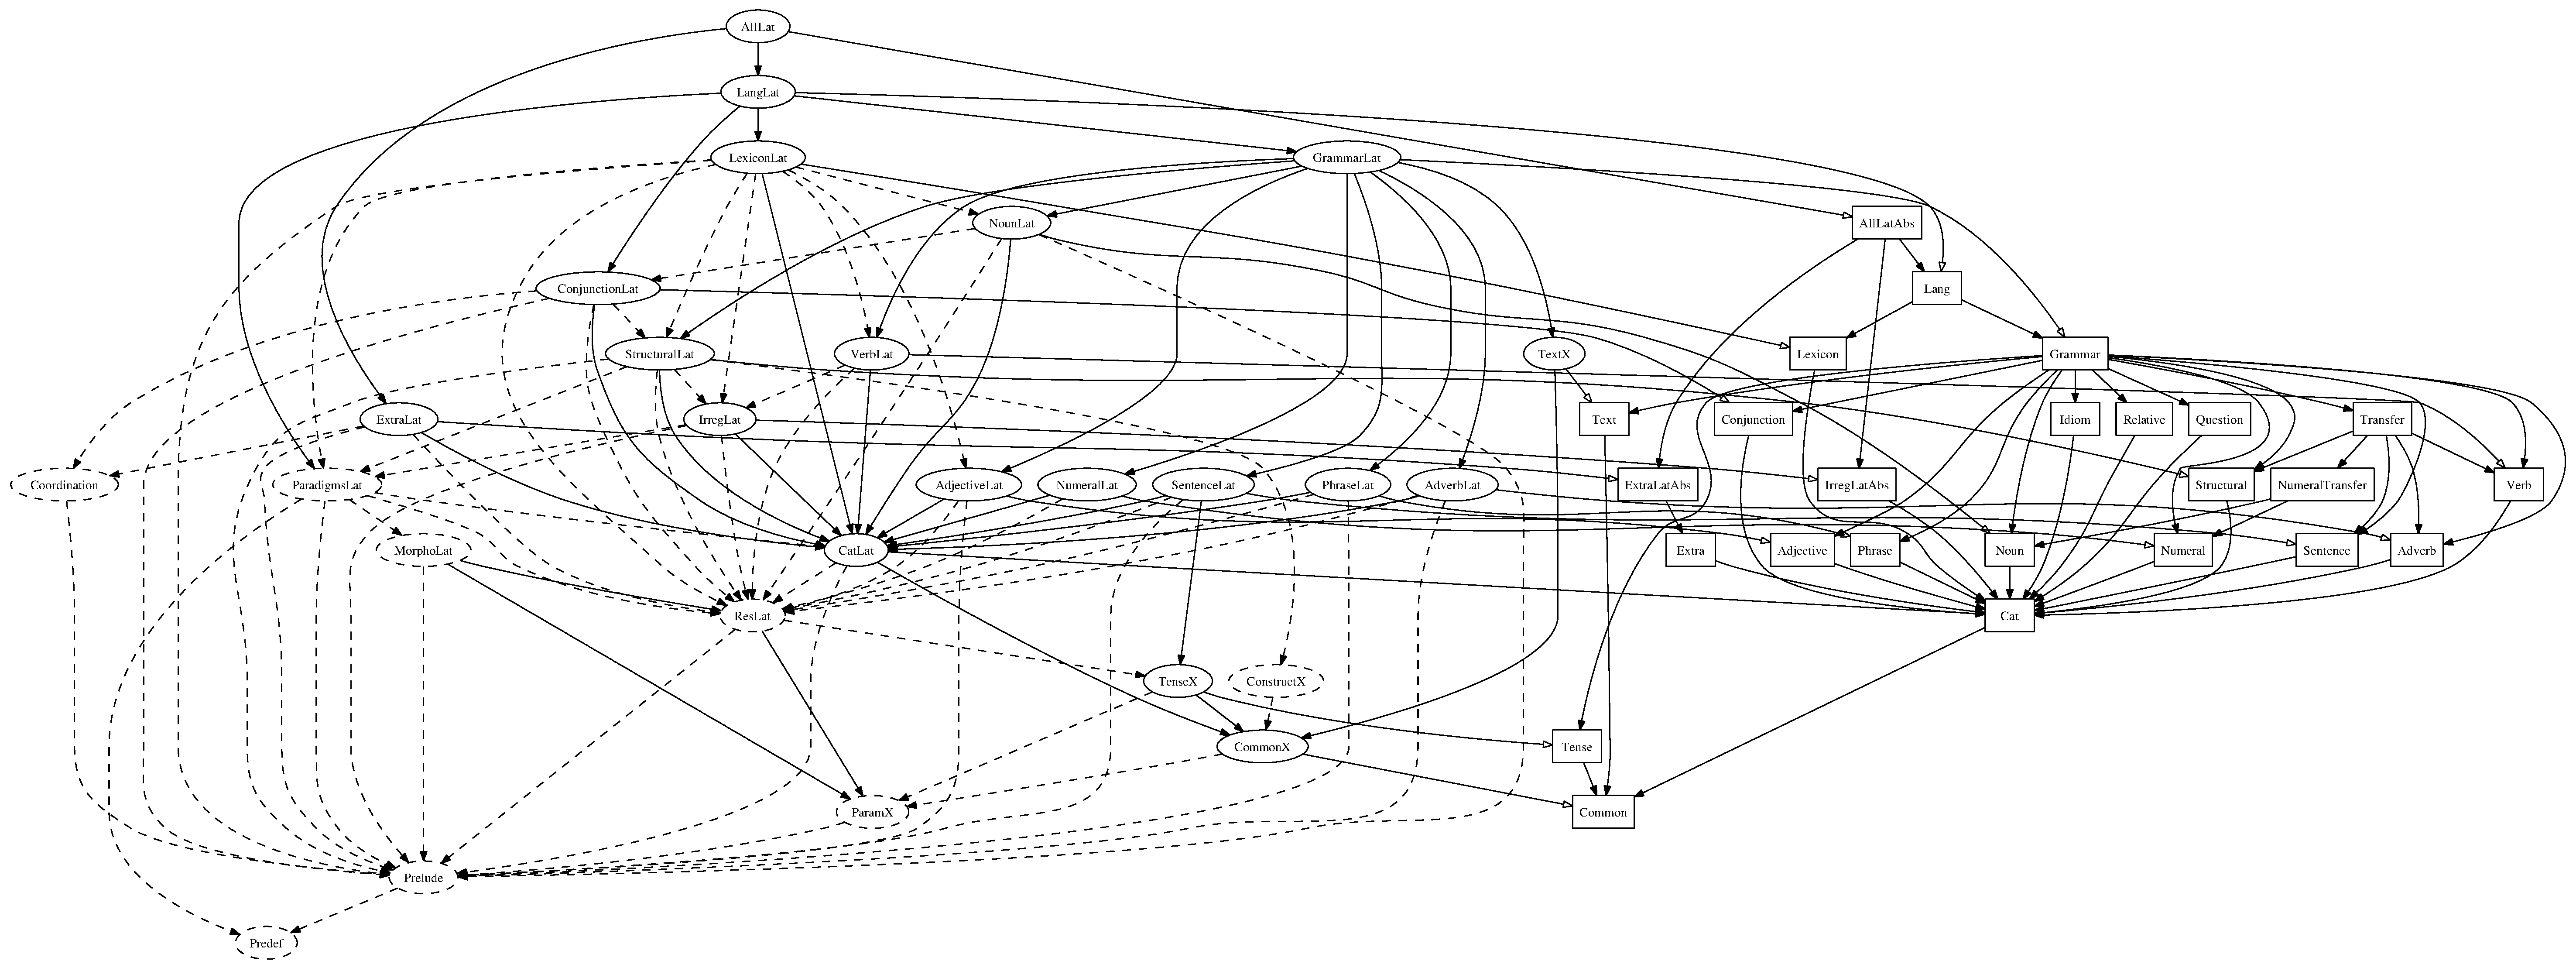
\includegraphics[scale=0.25]{graphics/LatinDependencyGraph.eps}
\caption{Die Abhängigkeiten zwischen den Modulen der Lateingrammatik}\label{GF-DepGraph}
\end{sidewaysfigure}
Nun kann man zum Testen entweder Testsätze parsen oder Sätze anhand der Grammatik erzeugen, um sie auch Korrektheit zu überprüfen. Zum Parsen existiert im Grammatical Framework der offensichtliche Befehl \texttt{parse}, dem eine Zeichenkette als Parameter übergeben wird und als Ergebnis eine Zeichenkette, die die entsprechenden abstrakten Syntaxbäume repräsentiert, zurückgibt. So kann z.B. der Satz \textit{feminae dormiunt} (deutsch: ``Die Frauen schlafen'' bzw. ``Frauen schlafen'') geparsed werden. Als Ergebnis erhält man dann die abstrakten Syntaxbäume in Listing \ref{GF-AbstractStrings}. 
\begin{lstlisting}[float=h!tp,caption={Abstrakte Syntaxrepräsentationen des Satzes \textit{feminae dormiunt}},label={GF-AbstractStrings},basicstyle=\small]
PhrUtt NoPConj (UttS (UseCl (TTAnt TPres ASimul) PPos (PredVP (DetCN (DetQuant \
  DefArt NumPl) (UseN woman_N)) (UseV sleep_V)))) NoVoc 
PhrUtt NoPConj (UttS (UseCl (TTAnt TPres ASimul) PPos (PredVP (DetCN (DetQuant \
  IndefArt NumPl) (UseN woman_N)) (UseV sleep_V)))) NoVoc
\end{lstlisting}
Mit dem Befehl \texttt{generate\_random} lassen sich dagegen zufällige abstrakte Bäume erzeugen, die mit dem Befehl \texttt{linearize} in einen lateinischen Satz linearisiert werden können. So erzeugt die Befehlsfolge \texttt{> generate\_random | linearize } einen zufälligen lateinischen Satz. Mit dem Befehl \texttt{generate\_trees} können alle Bäume einer Kategorie, bis zu einer gewissen Tiefe, meist der Tiefe von vier, generiert werden. So lassen sich zumindest theoretisch alle in der Grammatik möglichen Sätze bilden. Allerdings sind dies bei dieser Lateingrammatik, selbst bei einer Tiefe von vier, schon fast 70 Millionen Sätze. \par
Offensichtlich ist diese Lateingrammatik also bereits zu einem gewissen Grade benutzbar, jedoch gibt es noch großen Spielraum für Erweiterungen. Die Bereiche des Lexikons und der Morphologie sind bereits komplett entsprechend der abstrakten Syntax, die für eine Ressource Grammar vorgegeben ist, implementiert. Hier wäre es wohl am ehesten sinnvoll, die Ergebnisse, die bereits erzielt werden können zu bewerten, nach möglichen Fehlern zu suchen und diese zu korrigieren. So wären mögliche Fehler im Lexikon z.B. Übersetzungen, die im tatsächlichen Sprachgebrauch fast nie vorkommen oder viel seltener vorkommen als gleichbedeutende Wörter. In diesem Falle sollte die Übersetzung angepasst werden. Fehler in der Morphologie dagegen können dazu führen, dass entweder existierende Wortformen nicht analysiert werden können oder dass Wortformen falsch analysiert werden. Man kann nun unter anderem versuchen, unter Verwendung von Korpora, diese Fehler zu finden. Dies kann jedoch mit lagwieriger Arbeit verbunden sein, die nur unter Umständen nur wenig Verbesserung bringt. \par
Dagegen ist im Bereich der Syntax noch einiges an Arbeit nötig um den vollen Umfang zu erreichen. Viele interessante linguistische Phänomene warten noch darauf, umgesetzt zu werden, denn das Ziel dieser Arbeit war es, überhaupt in der Lage zu sein, lateinische Sätze bilden und analysieren zu können. So fehlen aktuell leider noch Relativsätze, Fragesätze, verschiedene Wortstellungen bei der \texttt{Phr}-Kategorie, Partizipialkonstruktionen, etc. nur um ein paar zu nennen. Dadurch, dass die Anzahl und Funktion der Regeln vorgegeben ist, sollte es aber im Anschluss an diese Arbeit relativ einfach sein, die Grammatik so zu verfollständigen, dass sie als vollständige Sprache in das Grammatical Framework aufgenommen werden kann. 
\section{Anwendung}
Eine Frage der man sich für die Zukunft ebenfalls widmen kann, ist die mögliche Anwendung dieser Lateingrammatik, vor allem, wenn sie in Zukunft noch in den genannten Bereichen erweitert werden sollte. Der Traum jedes Schülers und zugleich wohl der Albtraum der Lehrer wäre ein tatsächlich funktionierendes Lateinübersetzungsprogramm. Ob dieses Ziel, vor allem bei der Übersetzung literarischer und lyrischer Texte, erreicht werden kann, ist jedoch noch nicht abzusehen. Allerdings wäre es denkbar z.B. eine automatisch Übersetzungshilfe für lateinische Inschriften für interessierte Touristen anzubieten. Dafür wäre möglicherweise die Integration in eine Anwendung für moderne Mobiltelefone denkbar. Dies ist insofern möglich, da das Grammatical Framework in der Lage ist Grammatiken in ein portables Grammatikformat umzuwandeln, für das es, teils noch unvollständige, Bibliotheken für verschiedene Programmiersprachen, unter anderem auch Java, gibt. Dadurch ist die Möglichkeit der Benutzung einer PGF-Grammatik in einer Android-Anwendung gegeben. Ebenfalls wäre die Integration in ein Web-Angebot möglich, da auch hierfür Bibliotheken bereitgestellt werden.\footnote{vgl. \cite{RANTA2011} S. 166ff.} \par
Interessanter dürfte jedoch die Überlegung sein, inwieweit diese Lateingrammatik im Unterricht eingesetzt werden könnte. Denn die Verwendung des Computers in der Schule wird wohl auf Dauer zunehmen. Und deshalb müssen für verschiedenste Schulfächer Konzepte zur Einbindung neuer Medien erarbeitet werden, so auch für den Lateinunterricht. Und eben in diesem Bereich sind mögliche Anwendungen dieser Arbeit zu finden. Zum einen ist eine beliebte Beispielanwendung für die Mehrsprachigkeit des Grammatical Frameworks eine Webanwendung namens ``fridge poetry magnets'', bei der man wie aus Magneten am Kühlschrank auf die Wörter gedruckt sind, Sätze bilden kann, die allerdings anders als am Kühlschrank den Regeln einer Grammatik folgen müssen. Die so gebildeten Sätze können dann in verschiedene Sprachen übersetzt werden.\footnote{vgl. \cite{RANTA2011} S. 166} Auf diese Weise ist ein spielerischer Zugang zur lateinischen Sprache möglich, indem man z.B. deutsche Sätze baut und sich anschließend ansehen kann, wie eben dieser Satz auf Latein aussehen würde. Und wegen der Beschränkung, dass nur syntaktisch korrekte Sätze konstruiert werden können, kann man durch das zusammensetzen lateinischer Sätze möglicherweise spielerisch ein Sprachgefühl entwickeln. \par
Außerdem bietet das Grammatical Framework auch Möglichkeiten mit Hilfe einer Grammatik Übungsmöglichkeiten für eine Sprache zu bieten. Denn im Grammatical Framework ist die möglichkeit für sogenannte ``Quizes'' gegeben. Das erste dieser Fragespiele, das mit dem Befehl \texttt{morphology\_quiz} gestartet wird, fragt nach einer spezifischen Wortform eines Wortes einer gegebenen Kategorie, in dem es einem die Grundform und die gewünschten morphologischen Merkmale nennt. Eine Beispielsitzung ist in Listing \ref{GF-MorphoQuiz} zu sehen. Auf diese Weise lässt sich die lateinische Wortformenbildung üben.
\begin{lstlisting}[float=h!tp,caption={Eine Beispielsitzung des Grammatical Framework Morphology Quiz},label={GF-MorphoQuiz},basicstyle=\small]
> morphology_quiz -cat=N
Welcome to GF Morphology Quiz.
The quiz is over when you have done at least 10 examples
with at least 75 % success.

You can interrupt the quiz by entering a line consisting of a dot ('.').


navis s Pl Voc
> naves
Yes.
Score 1/1
plastica s Pl Nom
> plasticae
Yes.
Score 2/2
pulvis s Sg Voc
>
\end{lstlisting}
Um das Übersetzten auch abseits von Lehrbuchtexten zu üben stellt das Grammatical Framework analog zum ``Morphology Quiz'' ein ``Translation Quiz'' bereit. Um es zu verwenden müssen mindestens die Grammatiken zweier Sprachen geladen sein. Anschließend kann man unter Angabe der Quell- und Zielsprache ähnlich wie bei dem ``Morphology Quiz'' vom Programm vorgegebene Sätze übersetzen, wobei das Können wieder wie oben durch eine Punktzahl bewertet wird. Diese zwei eingebauten Übungsmöglichkeiten sind jedoch nur bedingt für den wirklichen Einsatz im Unterricht geeignet. Da das Grammatical Framework aber leicht in eigene Programme und Systeme integriert werden kann, bieten sich auch hier möglichkeiten zur weiteren Arbeit.\par
In dieser Arbeit wurden die am Anfang beschriebenen Ziele erreicht. Doch wie in diesem Abschnitt dargestellt wurde, bieten sich noch Möglichkeiten um an diese Arbeit anzuknüpfen. Dabei kann man sich entscheiden, ob man sich bemüht die Grammatik weiter zu verbessern oder sich lieber mit der konkreten Umsetzung einer oder mehrerer Verwendungsmöglichkeiten widmet. Für Interessierte bietet diese Arbeit aber auf jeden Fall Anregung und Grundlage für weiterer Beschäftigung.
\FloatBarrier
\pagebreak
\clearpage
\pagenumbering{roman}
\setcounter{page}{1}
%\chapter*{Bibliographie}
%\bibliographystyle{natdin}
\printbibliography
\pagebreak
\chapter*{Tabellen- und Abbildungsverzeichnis}
\addcontentsline{toc}{chapter}{Tabellen- und Abbildungsverzeichnis}
\listoftables
\listoffigures
\lstlistoflistings
%\nopagebreak[4]
%\listof{program}{Beispiele}
\chapter*{Lebenslauf}
\addcontentsline{toc}{chapter}{Lebenslauf}
\chapter*{Eigenständigkeitserklärung}
\addcontentsline{toc}{chapter}{Eigenständigkeitserklärung}
Hiermit versichere ich, dass ich die vorliegende Hausarbeit selbständig und ohne fremde Hilfe angefertigt, alle benutzten Quellen und Hilfsmittel angegeben und Zitate als solche kenntlich gemacht habe. \\
Ich versichere ferner, dass ich die Arbeit weder für eine Prüfung an einer weiteren Hochschule noch für eine staatliche Prüfung eingereicht habe. \par
\vspace{3cm}
München, den \rule{7cm}{0.4pt} \par
\vspace{3cm}
\rule{10cm}{0.4pt} \par
Herbert Lange
%\part{Anhang}
%\label{part:anhang}
%\section{Quelltext}
%\label{sec:quelltext}
%%\lstinputlisting[caption={Unterschiede zwischen der Anfangs- und Endversion der Lateingrammatik},label={GF-Adjective-Diff},basicstyle=\tiny]{complete.diff}
\lstinputlisting[caption={Unterschiede der Datei \texttt{AdjectiveLat.gf}},label={GF-Adjective-Diff},basicstyle=\tiny]{diffs/AdjectiveLat.gf.diff}
\lstinputlisting[caption={Unterschiede der Datei \texttt{AdverbLat.gf}},label={GF-Adverb-Diff},basicstyle=\tiny]{diffs/AdverbLat.gf.diff}
\lstinputlisting[caption={Unterschiede der Datei \texttt{AllLatAbs.gf}},label={GF-AllAbs-Diff},basicstyle=\tiny]{diffs/AllLatAbs.gf.diff}
\lstinputlisting[caption={Unterschiede der Datei \texttt{AllLat.gf}},label={GF-All-Diff},basicstyle=\tiny]{diffs/AllLat.gf.diff}
\lstinputlisting[caption={Unterschiede der Datei \texttt{CatLat.gf}},label={GF-Cat-Diff},basicstyle=\tiny]{diffs/CatLat.gf.diff}
\lstinputlisting[caption={Unterschiede der Datei \texttt{ConjunctionLat.gf}},label={GF-Conjunction-Diff},basicstyle=\tiny]{diffs/ConjunctionLat.gf.diff}
\lstinputlisting[caption={Unterschiede der Datei \texttt{ExtraLatAbs.gf}},label={GF-ExtraAbs-Diff},basicstyle=\tiny]{diffs/ExtraLatAbs.gf.diff}
\lstinputlisting[caption={Unterschiede der Datei \texttt{ExtraLat.gf}},label={GF-Extra-Diff},basicstyle=\tiny]{diffs/ExtraLat.gf.diff}
\lstinputlisting[caption={Unterschiede der Datei \texttt{GrammarLat.gf}},label={GF-Grammar-Diff},basicstyle=\tiny]{diffs/GrammarLat.gf.diff}
\lstinputlisting[caption={Unterschiede der Datei \texttt{IrregLatAbs.gf}},label={GF-IrregAbs-Diff},basicstyle=\tiny]{diffs/IrregLatAbs.gf.diff}
\lstinputlisting[caption={Unterschiede der Datei \texttt{IrregLat.gf}},label={GF-Irreg-Diff},basicstyle=\tiny]{diffs/IrregLat.gf.diff}
\lstinputlisting[caption={Unterschiede der Datei \texttt{LangLat.gf}},label={GF-Lang-Diff},basicstyle=\tiny]{diffs/LangLat.gf.diff}
\lstinputlisting[caption={Unterschiede der Datei \texttt{LexiconLat.gf}},label={GF-Lexicon-Diff},basicstyle=\tiny]{diffs/LexiconLat.gf.diff}
\lstinputlisting[caption={Unterschiede der Datei \texttt{MorphoLat.gf}},label={GF-Morpho-Diff},basicstyle=\tiny]{diffs/MorphoLat.gf.diff}
\lstinputlisting[caption={Unterschiede der Datei \texttt{NounLat.gf}},label={GF-Noun-Diff},basicstyle=\tiny]{diffs/NounLat.gf.diff}
%\lstinputlisting[caption={Unterschiede der Datei \texttt{NumeralLat.gf}},label={GF-Numeral-Diff},basicstyle=\tiny]{diffs/NumeralLat.gf.diff}
\lstinputlisting[caption={Unterschiede der Datei \texttt{ParadigmsLat.gf}},label={GF-Paradigms-Diff},basicstyle=\tiny]{diffs/ParadigmsLat.gf.diff}
\lstinputlisting[caption={Unterschiede der Datei \texttt{PhraseLat.gf}},label={GF-Phrase-Diff},basicstyle=\tiny]{diffs/PhraseLat.gf.diff}
%\lstinputlisting[caption={Unterschiede der Datei \texttt{QuestionLat.gf}},label={GF-Question-Diff},basicstyle=\tiny]{diffs/QuestionLat.gf.diff}
%\lstinputlisting[caption={Unterschiede der Datei \texttt{RelativeLat.gf}},label={GF-Relativ-Diff},basicstyle=\tiny]{diffs/RelativeLat.gf.diff}
\lstinputlisting[caption={Unterschiede der Datei \texttt{ResLat.gf}},label={GF-Res-Diff},basicstyle=\tiny]{diffs/ResLat.gf.diff}
\lstinputlisting[caption={Unterschiede der Datei \texttt{SentenceLat.gf}},label={GF-Senctence-Diff},basicstyle=\tiny]{diffs/SentenceLat.gf.diff}
\lstinputlisting[caption={Unterschiede der Datei \texttt{StructuralLat.gf}},label={GF-Structural-Diff},basicstyle=\tiny]{diffs/StructuralLat.gf.diff}
%\lstinputlisting[caption={Unterschiede der Datei \texttt{SymbolLat.gf}},label={GF-Symbol-Diff},basicstyle=\tiny]{diffs/SymbolLat.gf.diff}
\lstinputlisting[caption={Unterschiede der Datei \texttt{VerbLat.gf}},label={GF-Verb-Diff},basicstyle=\tiny]{diffs/VerbLat.gf.diff}
\end{document}
